%!TEX root = ../thesis.tex

\chapter{闪电二氧化氮反演算法的应用} \label{chapter:PE}

由于LNO$_2$不仅存在于对流旺盛期,也可在对流初生和消散阶段出现NO$_2$高值,
因此本章在第\ref{chapter:retrieval}章开发的LNO$_2$反演算法基础之上,
计算并比较污染地区(中国东部)和清洁地区(北极)不同阶段对流的LNO$_2$产率。
其中TROPOMI在北极地区的连续过境特性,可为将来静止化学监测卫星在LNO$_2$的研究中提供可靠的依据。

本章余下部分按照以下方式组织:
\ref{sec:china}节在第\ref{chapter:retrieval}章的基础上计算中国东部对流在消散阶段的LNO$_{\ch{2}}$柱浓度和产率,
并分析LNO$_2$对于TROPOMI NO$_{\ch{2}}$柱浓度产品的影响;
\ref{sec:arctic}节利用TROPOMI在北极地区的相邻过境数据,
计算LNO$_{\ch{2}}$的产率和产量,分析其海陆性差异,
并与其他NO$_{\ch{x}}$排放源进行对比;
最后是本章小结。


\section{污染地区(中国东部)} \label{sec:china}

\subsection{模式设置及闪电同化结果评估} \label{sec:model_settings_china}

中国东部的研究使用的WRF-Chem版本号为4.1.4,气象条件的初始场和边界场来自1小时分辨率的ERA5再分析资料。
模式的垂直分层为75层,对流层顶设置为50 hPa,嵌套区域如图\ref{fig:domains_china}所示。
微物理过程使用WSM6方案\citep{Hong.2006a},而短波和长波辐射使用RRTMG方案\citep{Iacono.2008},陆面过程由Noah方案模拟\citep{Koren.1999}。
但是,本研究使用不同的边界层参数化来模拟两次对流个例,2019年的个例使用YSU方案\citep{Hong.2006},2020年的个例使用QNSE方案\citep{Sukoriansky.2005}。

化学初始场和边界场采用整个大气社区气候模式(WACCM)的输出数据。
其中2020年个例的O$_{\ch{3}}$初始场使用臭氧探空仪观测所得的O$_{\ch{3}}$廓线。
人为排放使用2016年中国多分辨率排放清单(MEIC)1.3版,
生物排放采用来自自然界的气体和气溶胶排放模型[MEGAN,\citet{Guenther.2006}]。
化学方案使用气相化学的臭氧和相关化学示踪剂模式(MOZART)和气溶胶的Goddard化学气溶胶辐射和传输(GOCART)模式\citep{Pfister.2011}。
其中光解方案采用基于云光学厚度(cloud\_fraction$^{1.5}$)的新对流层紫外线和可见光(TUV)方案,即光解速率依赖于气溶胶和云。
此外LNO的垂直廓线使用\citet{Ott.2010}的双峰型LNO廓线\citep{Laughner.2017},而LNO和LNO$_{\ch{2}}$廓线是指开启和关闭LNO排放的模拟垂直廓线的差异,
其中LNO$_{\ch{x}}$参数化调整为每次闪电产生500 mol NO \citep{Zhu.2019}。


\begin{figure}[H]
\centering
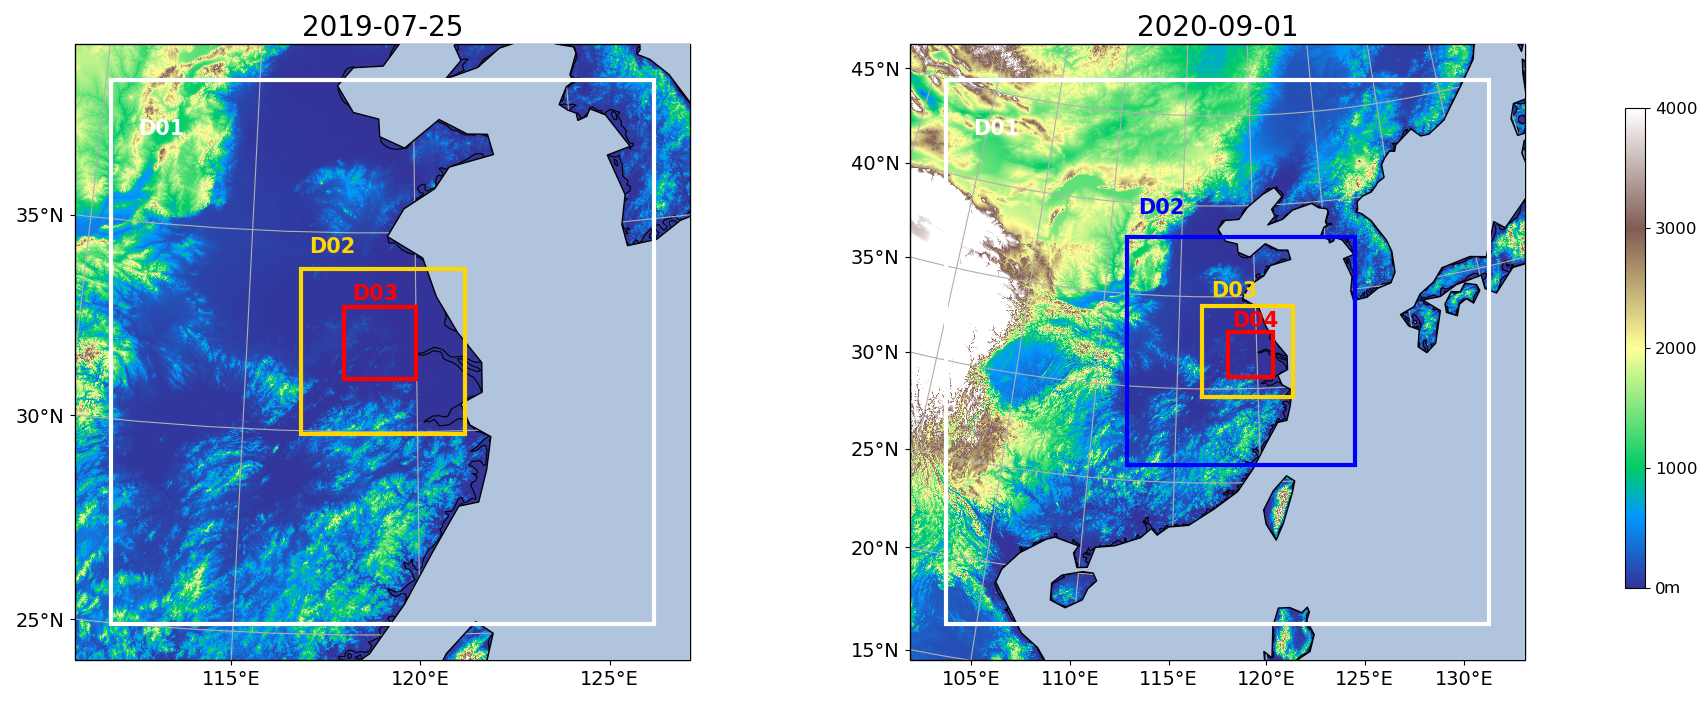
\includegraphics[width=\textwidth]{./figures/domains_china.png}
\caption{2019年和2020年个例的WRF-Chem模拟区域和地形高度(m)图。
2019年个例的水平网格分辨率为15 km(D01)、3 km(D02)和 0.6 km(D03)。
对于2020年个例,分别为27 km(D01)、9 km(D02)、3 km(D03)和 1 km(D04)。\\
Figure \ref{fig:domains_china}. Domain and terrain height (m) of the WRF-Chem simulations for the 2019 and 2020 cases. The horizontal grid resolution of
domains for the 2019 case is 15 km (D01), 3 km (D02) and 0.6 km (D03). For the 2020 case, it is 27 km (D01), 9 km (D02), 3 km (D03),
and 1 km (D04).}
\label{fig:domains_china}
\end{figure}

由于中国东部的对流生命期短,本研究采用了闪电同化并利用晴空条件下的臭氧探空资料修正了O$_{\ch{3}}$初始场,然后将模拟结果与探空和雷达对比。
闪电数据同化方法详见\citet{Fierro.2012}和\citet{Li.2017b},主要步骤为在闪电所处网格的垂直恒温层间,增加水汽质量混合比:
\begin{equation} \label{eq:lda}
Q_{v}=A Q_{\ch{sat}}+B Q_{\ch{sat}} \tanh (C X)\left[1-\tanh \left(D Q_{g}^{\alpha}\right)\right]
\end{equation}
其中Q$_{\ch{sat}}$ 为水汽饱和混合比(g kg$^{−1}$),Q$_g$为霰粒混合比(g kg$^{−1}$),X 为闪电频率。
本研究选择263.15 K和 290.15 K作为恒温层的上下限,其目的是为了让对流在行星边界层中快速扎根\citep{Marchand.2014,Finney.2016,Li.2017b}。
参数设置参考\citet{Li.2017b}:A=0.94,B=0.2,C=0.001,D=0.25,α=2.2。
其中网格化的总闪数据通过WRF的辅助输入流进行每10分钟的读取。
例如,如果闪电同化开始于05:00 UTC,时间步长为10 min,则将05:00--05:10 UTC之间特定网格中所有闪电数相加作为此期间的贡献。
在下一个时间步长,闪电被归类为下一个新组。
因此,该闪电数实际为闪电频率的密度(单位:闪电数 每10 min 每dx km 每dy km),其中dx和dy分别是模式网格在x和y方向的分辨率。
如\citet{Fierro.2012}和\citet{Li.2017b}所述,这可以确保所有嵌套层中的闪电密度相同。
此外,闪电数也直接同化进WRF-Chem中,该方法已应用于社区多尺度空气质量[CMAQ,\citet{Kang.2019a,Kang.2019,Kang.2020}]模式中。


\begin{figure}[H]
\centering
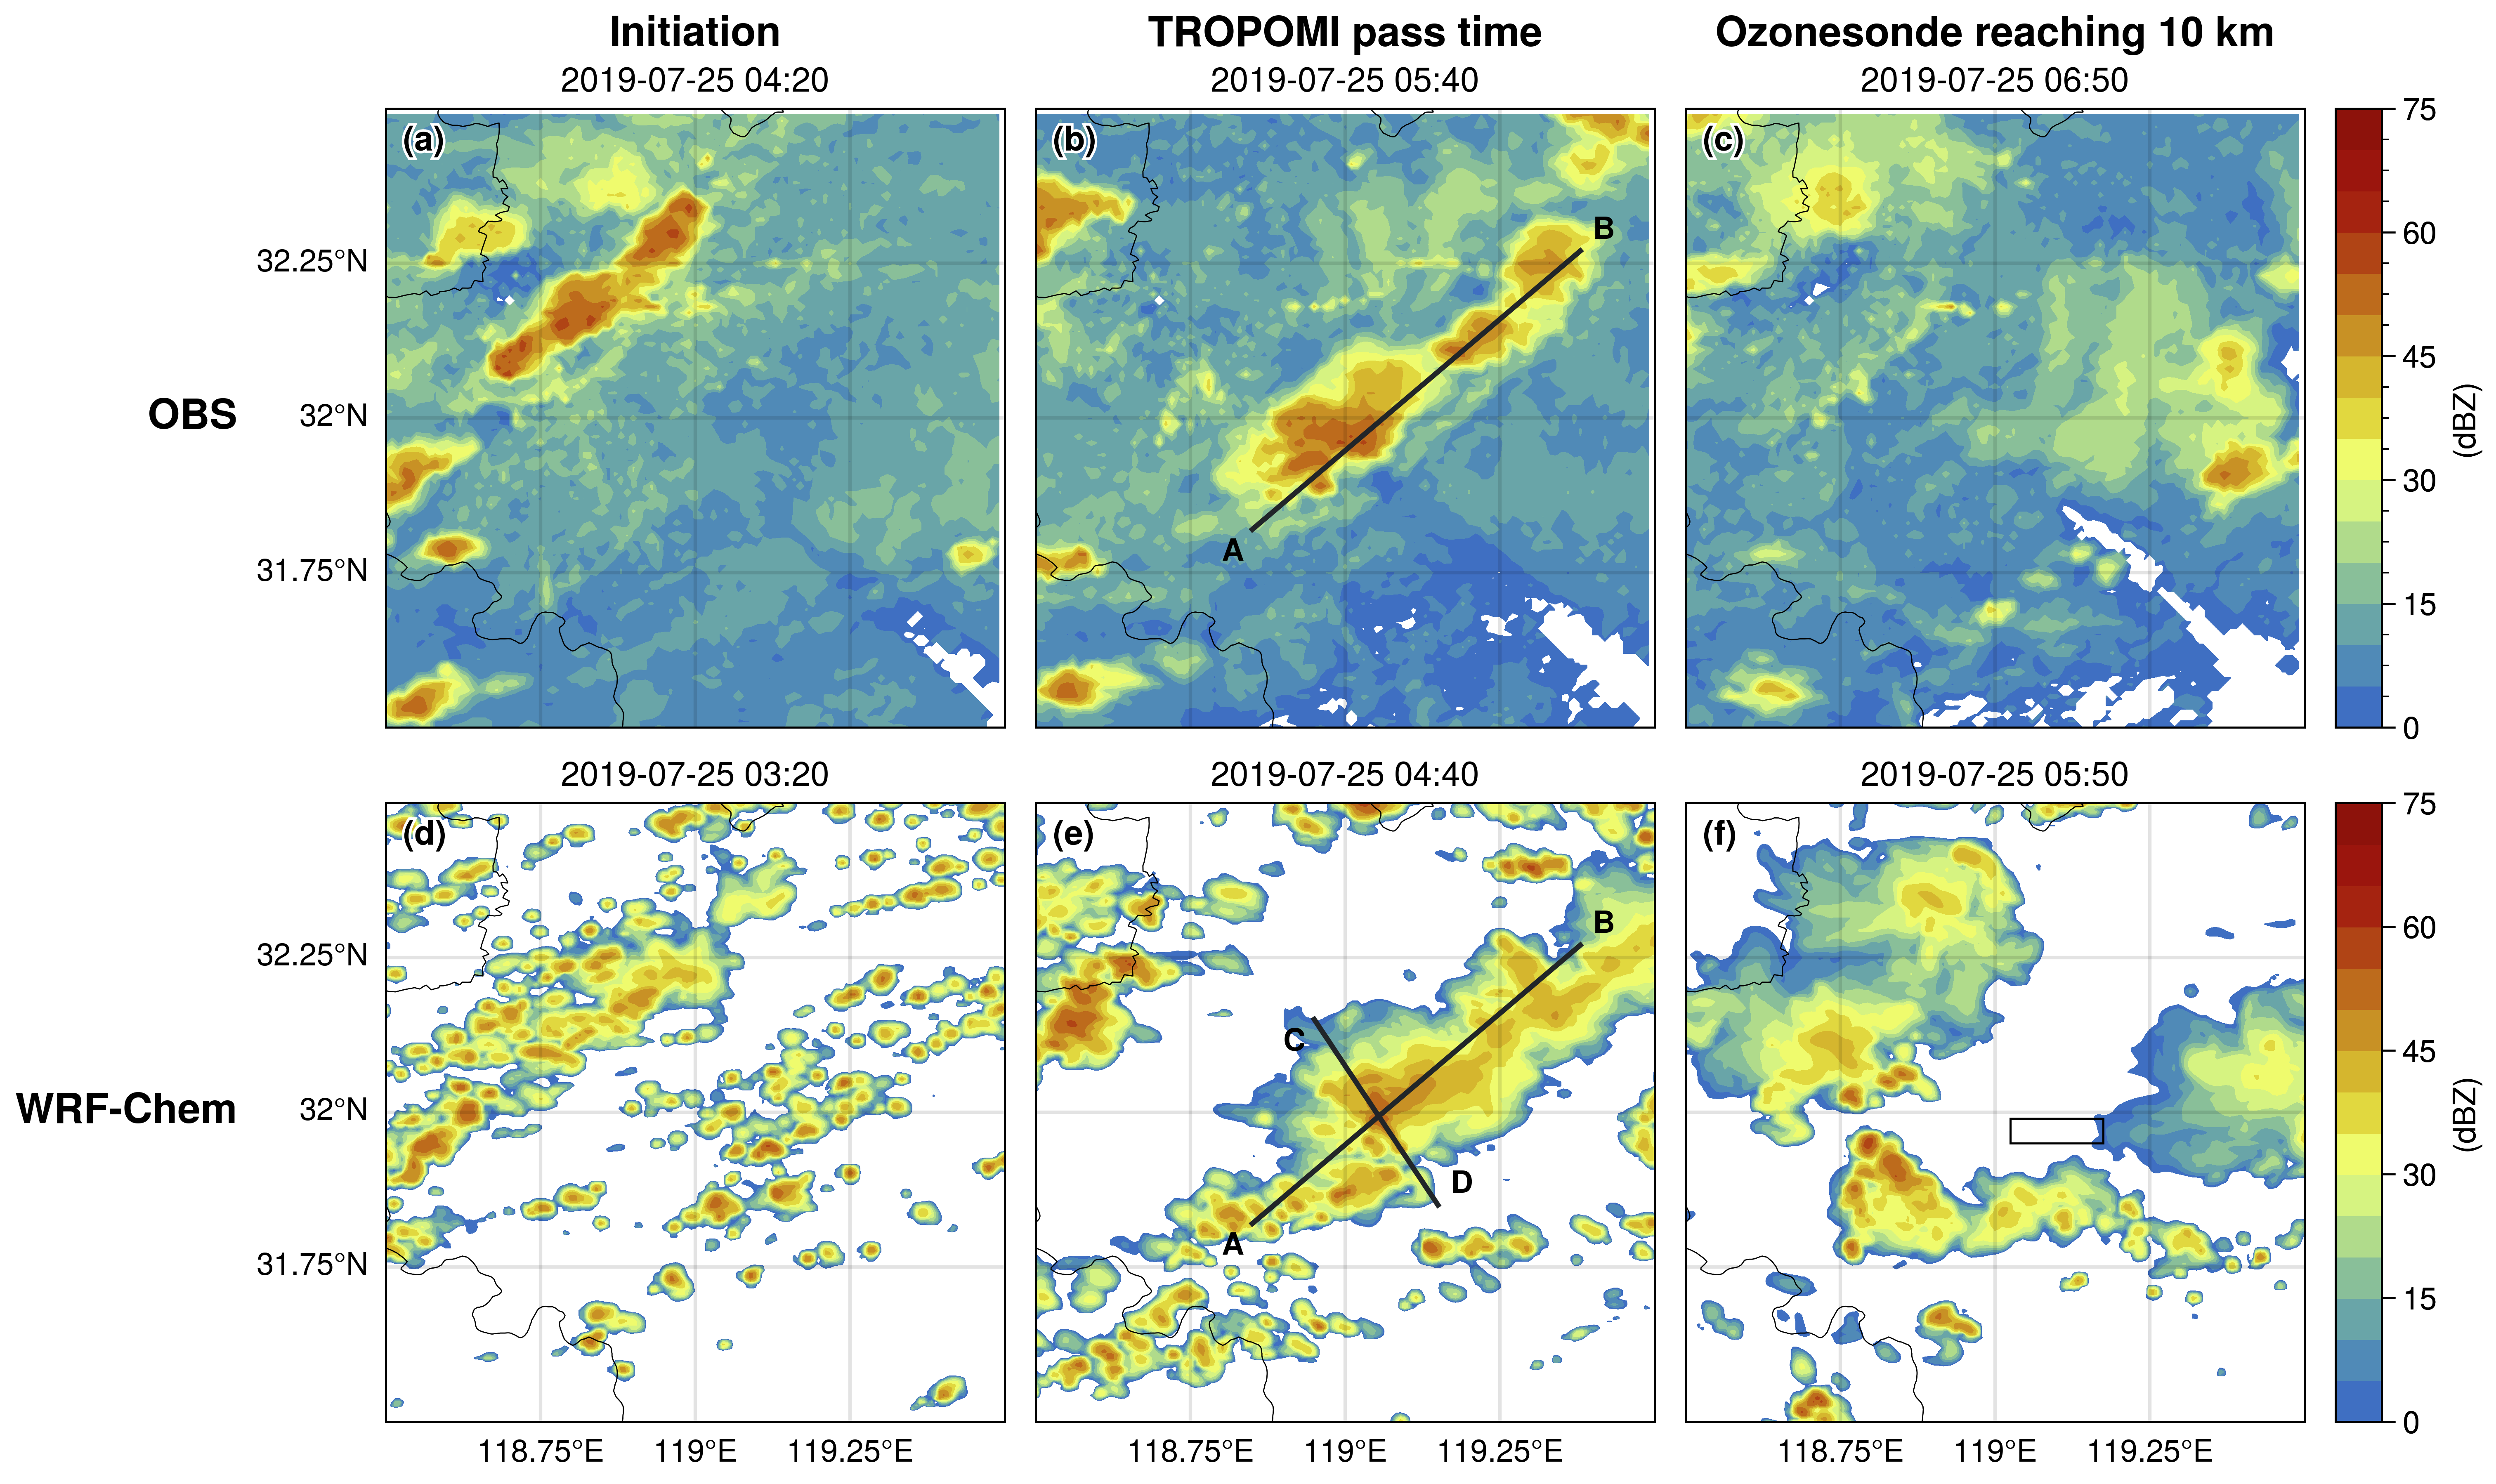
\includegraphics[width=\textwidth]{./figures/comp_crf_2019.png}
\caption{于(a)04:20 UTC、(b)05:40 UTC 和(c)06:50 UTC 观测到的雷达组合反射率;
         (d--e)WRF-Chem 在雷达观测时间前一小时模拟的雷达组合反射率;
         (b)和(e)中的 AB 实线是图 \ref{fig:comp_dbzcross_2019} 的剖面线;
         (e)中的CD实线是图\ref{fig:tendency_o3}b的剖面线。
         黑色矩形是与臭氧探空仪进行比较的区域。\\
         Figure \ref{fig:comp_crf_2019}. Observed radar composite reflectivity at (a) 04:20 UTC, (b) 05:40 UTC, and (c) 06:50 UTC.
        (d--e) WRF-Chem simulated composite reflectivity one hour before the radar observation times.
        The AB solid lines in (b) and (e) are cross section lines for Fig. \ref{fig:comp_dbzcross_2019}.
        The CD solid line in (e) is the cross section line for Fig. \ref{fig:tendency_o3}b.
        The black rectangle is the region for the comparison with ozonesonde.}
\label{fig:comp_crf_2019}
\end{figure}


与雷达观测相比,2019年7月25日和2020年9月1日模拟的对流初生时间,较实际观测分别提前了60和30分钟(图\ref{fig:comp_crf_2019}和图\ref{fig:comp_crf_2020}),所以闪电数据也以相同的时间间隔提前同化。
对于下文的结果比较,本研究选择匹配的阶段而不是相同的时间。

2019年7月25日的热对流在初始时呈现为孤立的热泡,WRF-Chem再现了初始阶段孤立对流的位置和强度(图\ref{fig:comp_crf_2019}a和\ref{fig:comp_crf_2020}d)。
对流系统在05:40 UTC时呈现东北--西南向,最大组合雷达反射率达到60 dBZ(图\ref{fig:comp_crf_2019}b),强度大于模拟的对流(最大组合雷达反射率为55 dBZ,图\ref{fig:comp_crf_2019}e)。
将模拟的对流核心区雷达反射率垂直剖面与观测结果进行对比(图\ref{fig:comp_dbzcross_2019}),
虽然对流距雷达过远造成缺失数据较多,但是在未进行人工插值的条件下,孤立对流的水平和垂直结构仍大致显示:
模拟的45 dBZ等值线达到12 km,但由于10 km 以上的数据质量低,
观测到的45 dBZ等值线仅达到10 km。

2020年9月1日观测到的飑线在北部初生,然后加强并向观测点移动(图\ref{fig:comp_crf_2020})。
对流旺盛阶段(最大组合雷达反射率为60 dBZ)大致在05:50 UTC,与TROPOMI过境时间相符(图\ref{fig:comp_dbzcross_2020}b,e)。
虽然该飑线抵达的最高高度低于2019年的热对流,但对流层低层(2--8 km)的反射率更大更广(图\ref{fig:comp_dbzcross_2020})。
由于模拟的对流消散区偏离了雷达观测的消散区,这导致与臭氧探空仪比较的区域设置在站点的西侧(图\ref{fig:comp_dbzcross_2020}c,f)。


\begin{figure}[H]
\centering
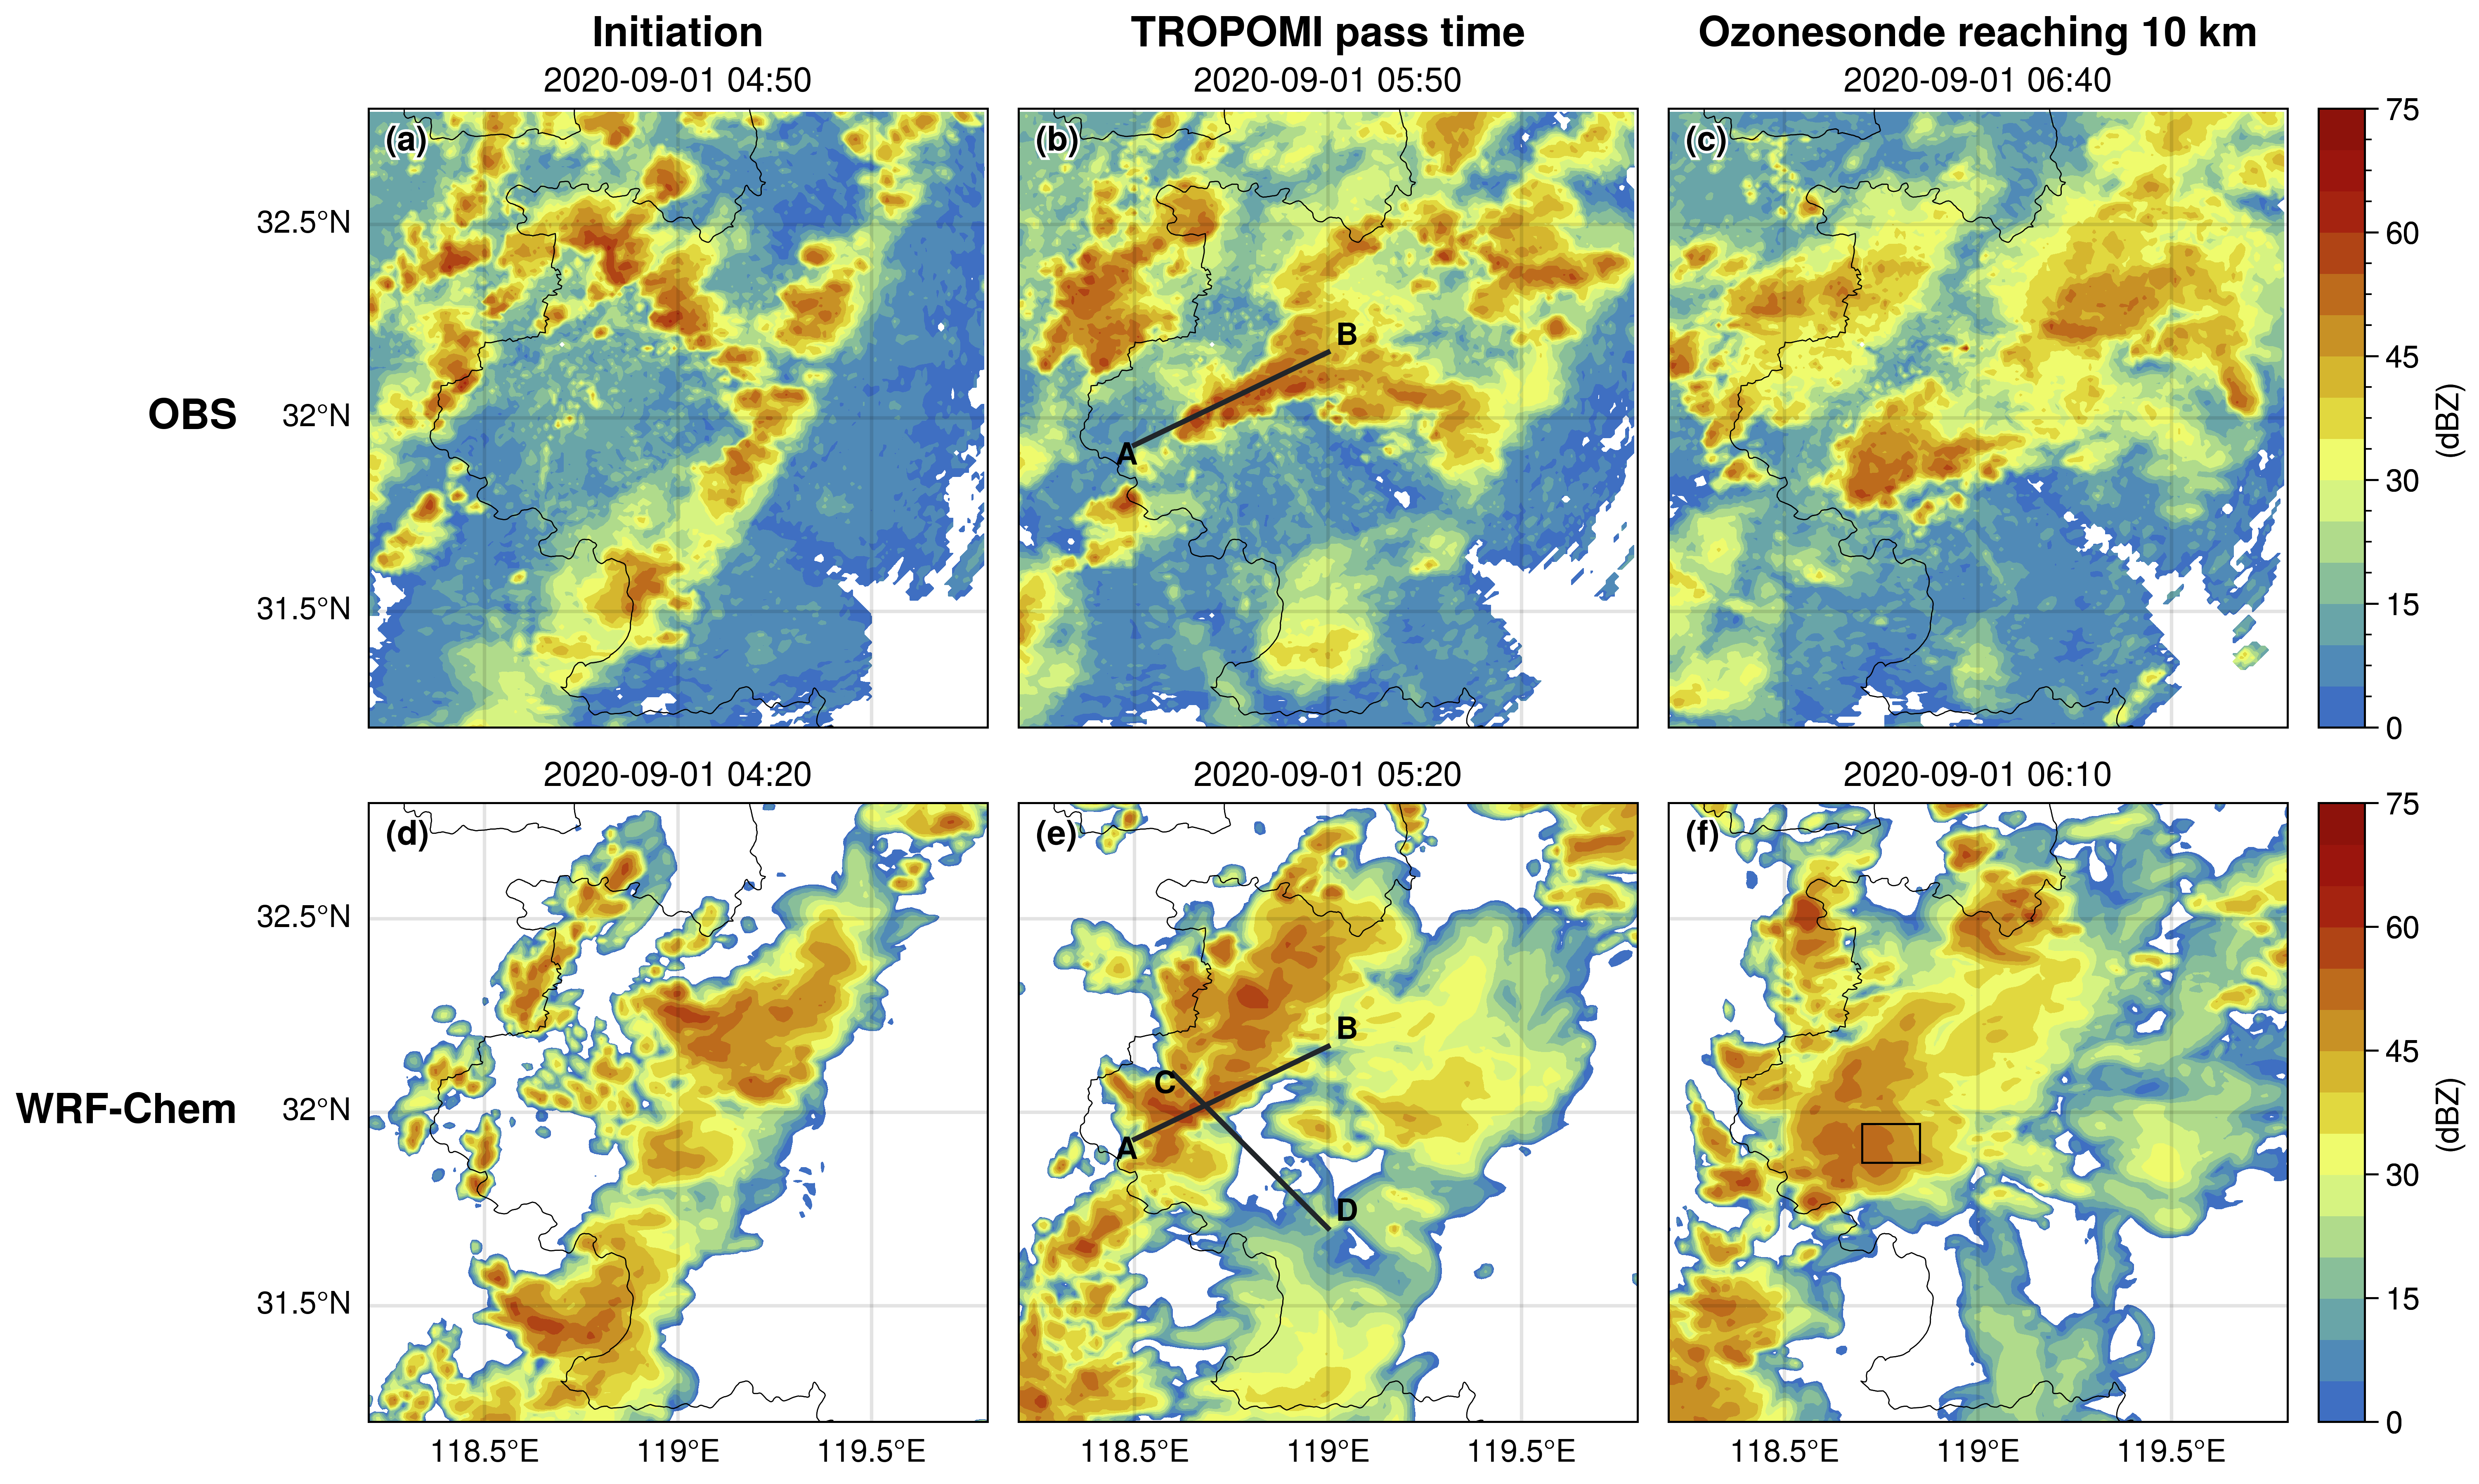
\includegraphics[width=\textwidth]{./figures/comp_crf_2020.png}
\caption{与图\ref{fig:comp_crf_2019} 相同,但针对2020年9月1日的对流个例,模拟时间比雷达观测提前30分钟。\\
Figure \ref{fig:comp_crf_2020}. Same as Fig. \ref{fig:comp_crf_2019} but for the case on 01 September 2020.
The simulation time is 30 minutes ahead of each radar observation.}
\label{fig:comp_crf_2020}
\end{figure}

\subsection{闪电氮氧化物的产率及其不确定性分析}


图\ref{fig:china_flash_scd}a--d将对流层NO$_{\ch{2}}$斜柱浓度($S_{\ch{NO2}}$)的分布与观测的闪电分布进行了比较。
尽管由于探测器饱和和光晕效应,闪电最活跃像素上的$S_{\ch{NO2}}$无效,但对流附近或出流区仍有有效数据。
在2019年的个例中,闪电发生在TROPOMI过境前不到30分钟,
但2020年的个例中既有新生也有老化的LNO$_{\ch{2}}$(图\ref{fig:china_flash_scd}d)。

具体而言,对流旺盛处(f$_r$ $\geq$ 0.7)的$S_{\ch{NO2}}$小于其他区域,
这与之前针对具有高闪电密度的大规模对流系统研究结果相反\citep{Beirle.2009},
导致这一差距的因素有四点:云顶高度、闪电次数、闪电发生时间和背景NO$_{\ch{2}}$浓度。
由于TROPOMI只能探测到处于云层上方的LNO$_{\ch{2}}$,因此当f$_r$ $\sim$ 1时,
闪电次数不足或对流较弱都可能导致对流旺盛区的$S_{\ch{NO2}}$更小。
即如果f$_r$<1,破碎或稀薄云层下方的部分污染NO$_{\ch{2}}$会被TROPOMI探测到。
WRF-Chem的先验$S_{\ch{NO2}}$敏感性试验可以清楚地解释这种现象:
具有低f$_r$和高$S_{\ch{NO2}}$的像素源自于背景 NO$_{\ch{2}}$ 污染(图\ref{fig:s5p_apriori_scd} a,e),
但与没有LNO$_{\ch{2}}$贡献的$S_{\ch{NO2}}$低值相比,
由对流层上层LNO$_{\ch{2}}$排放所增加的$S_{\ch{NO2}}$仍然清晰可见(图\ref{fig:s5p_apriori_scd}b--d,f--h)。


\begin{figure}[H]
\centering
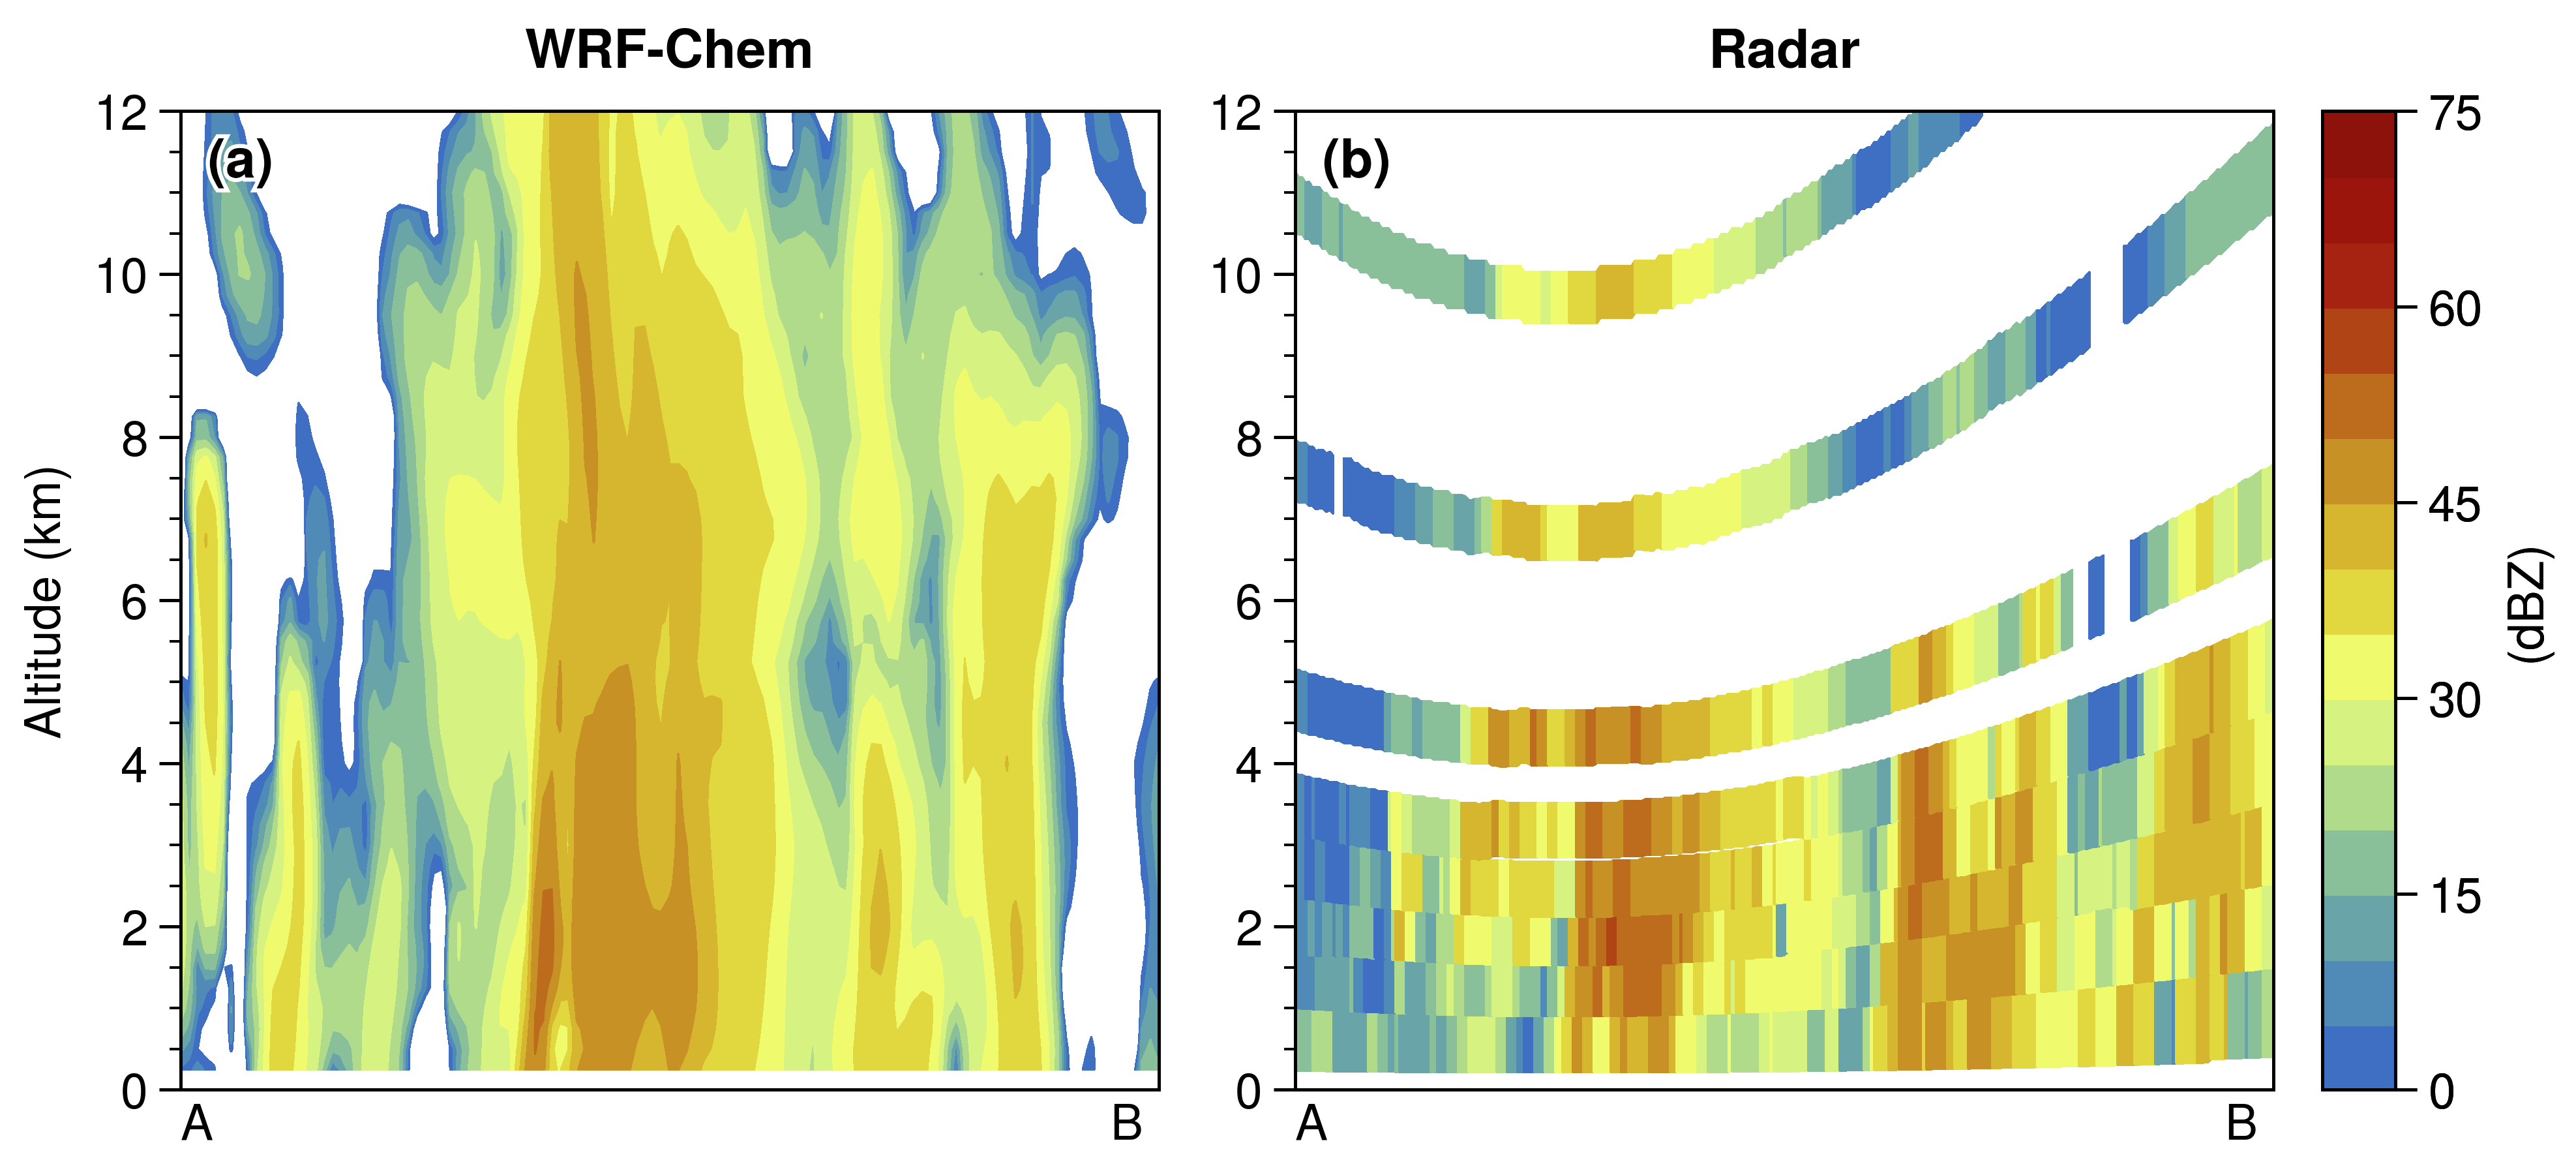
\includegraphics[width=\textwidth]{./figures/comp_dbzcross_2019.png}
\caption{沿着图\ref{fig:comp_crf_2019}中AB线剖得的2019年7月25日(a)WRF-Chem模拟和(b)雷达观测的雷达反射率。\\
Figure \ref{fig:comp_dbzcross_2019}. Vertical cross sections of (a) WRF-Chem simulated and (b) observed radar reflectivity fields along the transect lines (AB) in Fig. \ref{fig:comp_crf_2019} for 25 July, 2019.}
\label{fig:comp_dbzcross_2019}
\end{figure}

\begin{figure}[H]
\centering
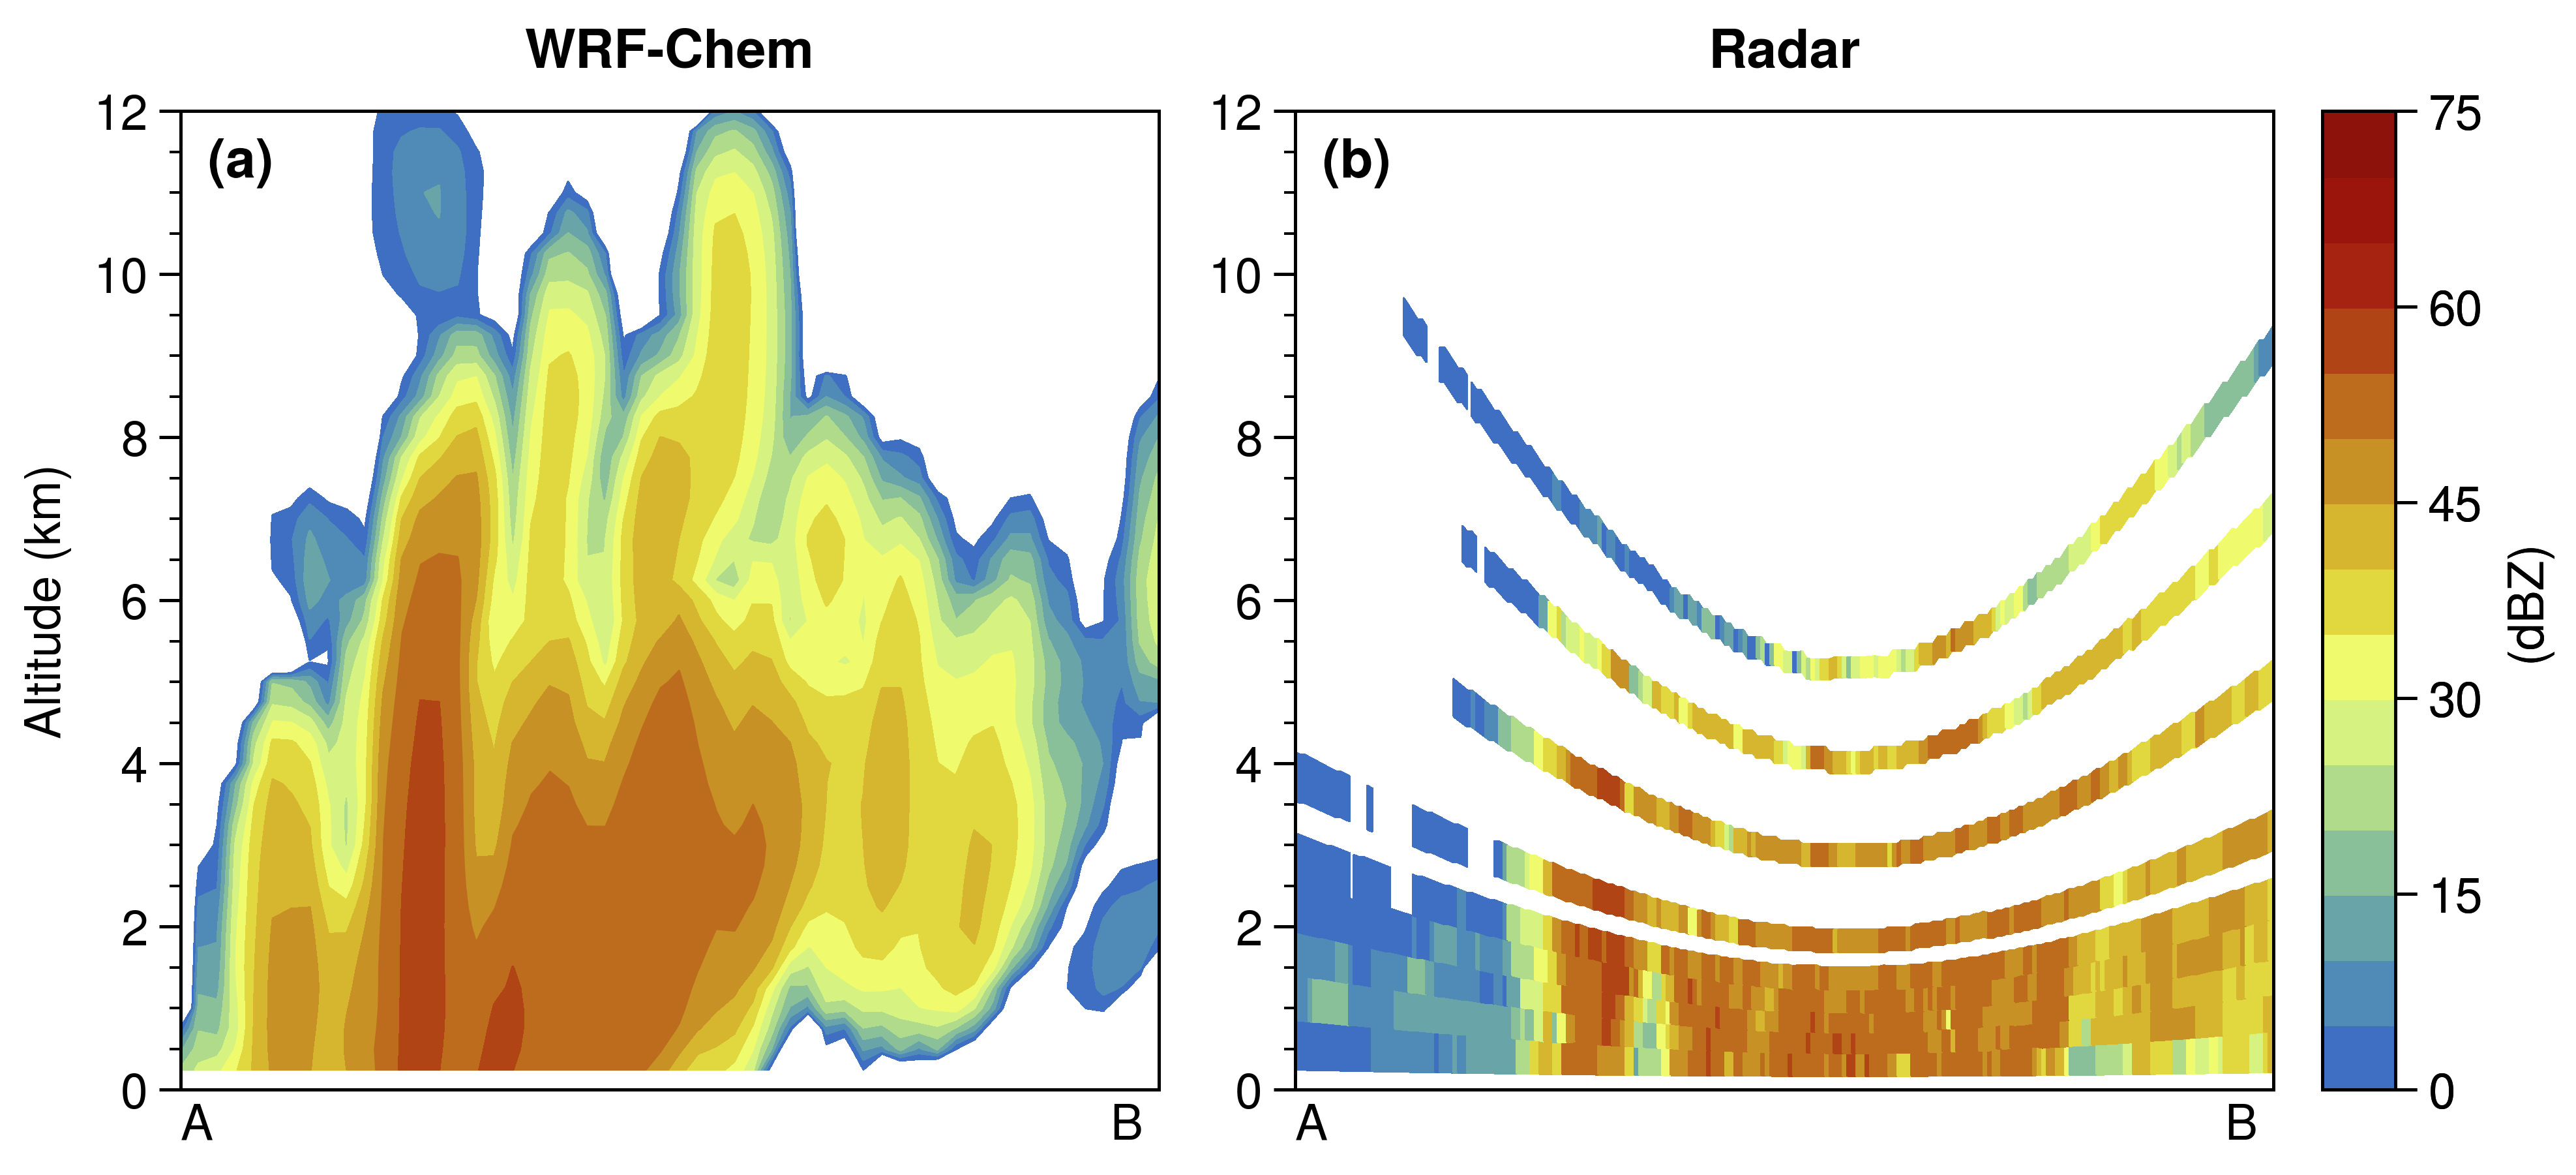
\includegraphics[width=\textwidth]{./figures/comp_dbzcross_2020.png}
\caption{与图\ref{fig:comp_dbzcross_2019}相同,但针对2020年9月1日的对流个例。\\
Figure \ref{fig:comp_dbzcross_2020}. Same as Figure \ref{fig:comp_dbzcross_2019} but for the case on 01 September 2020.}
\label{fig:comp_dbzcross_2020}
\end{figure}



\begin{figure}[H]
    \centering
    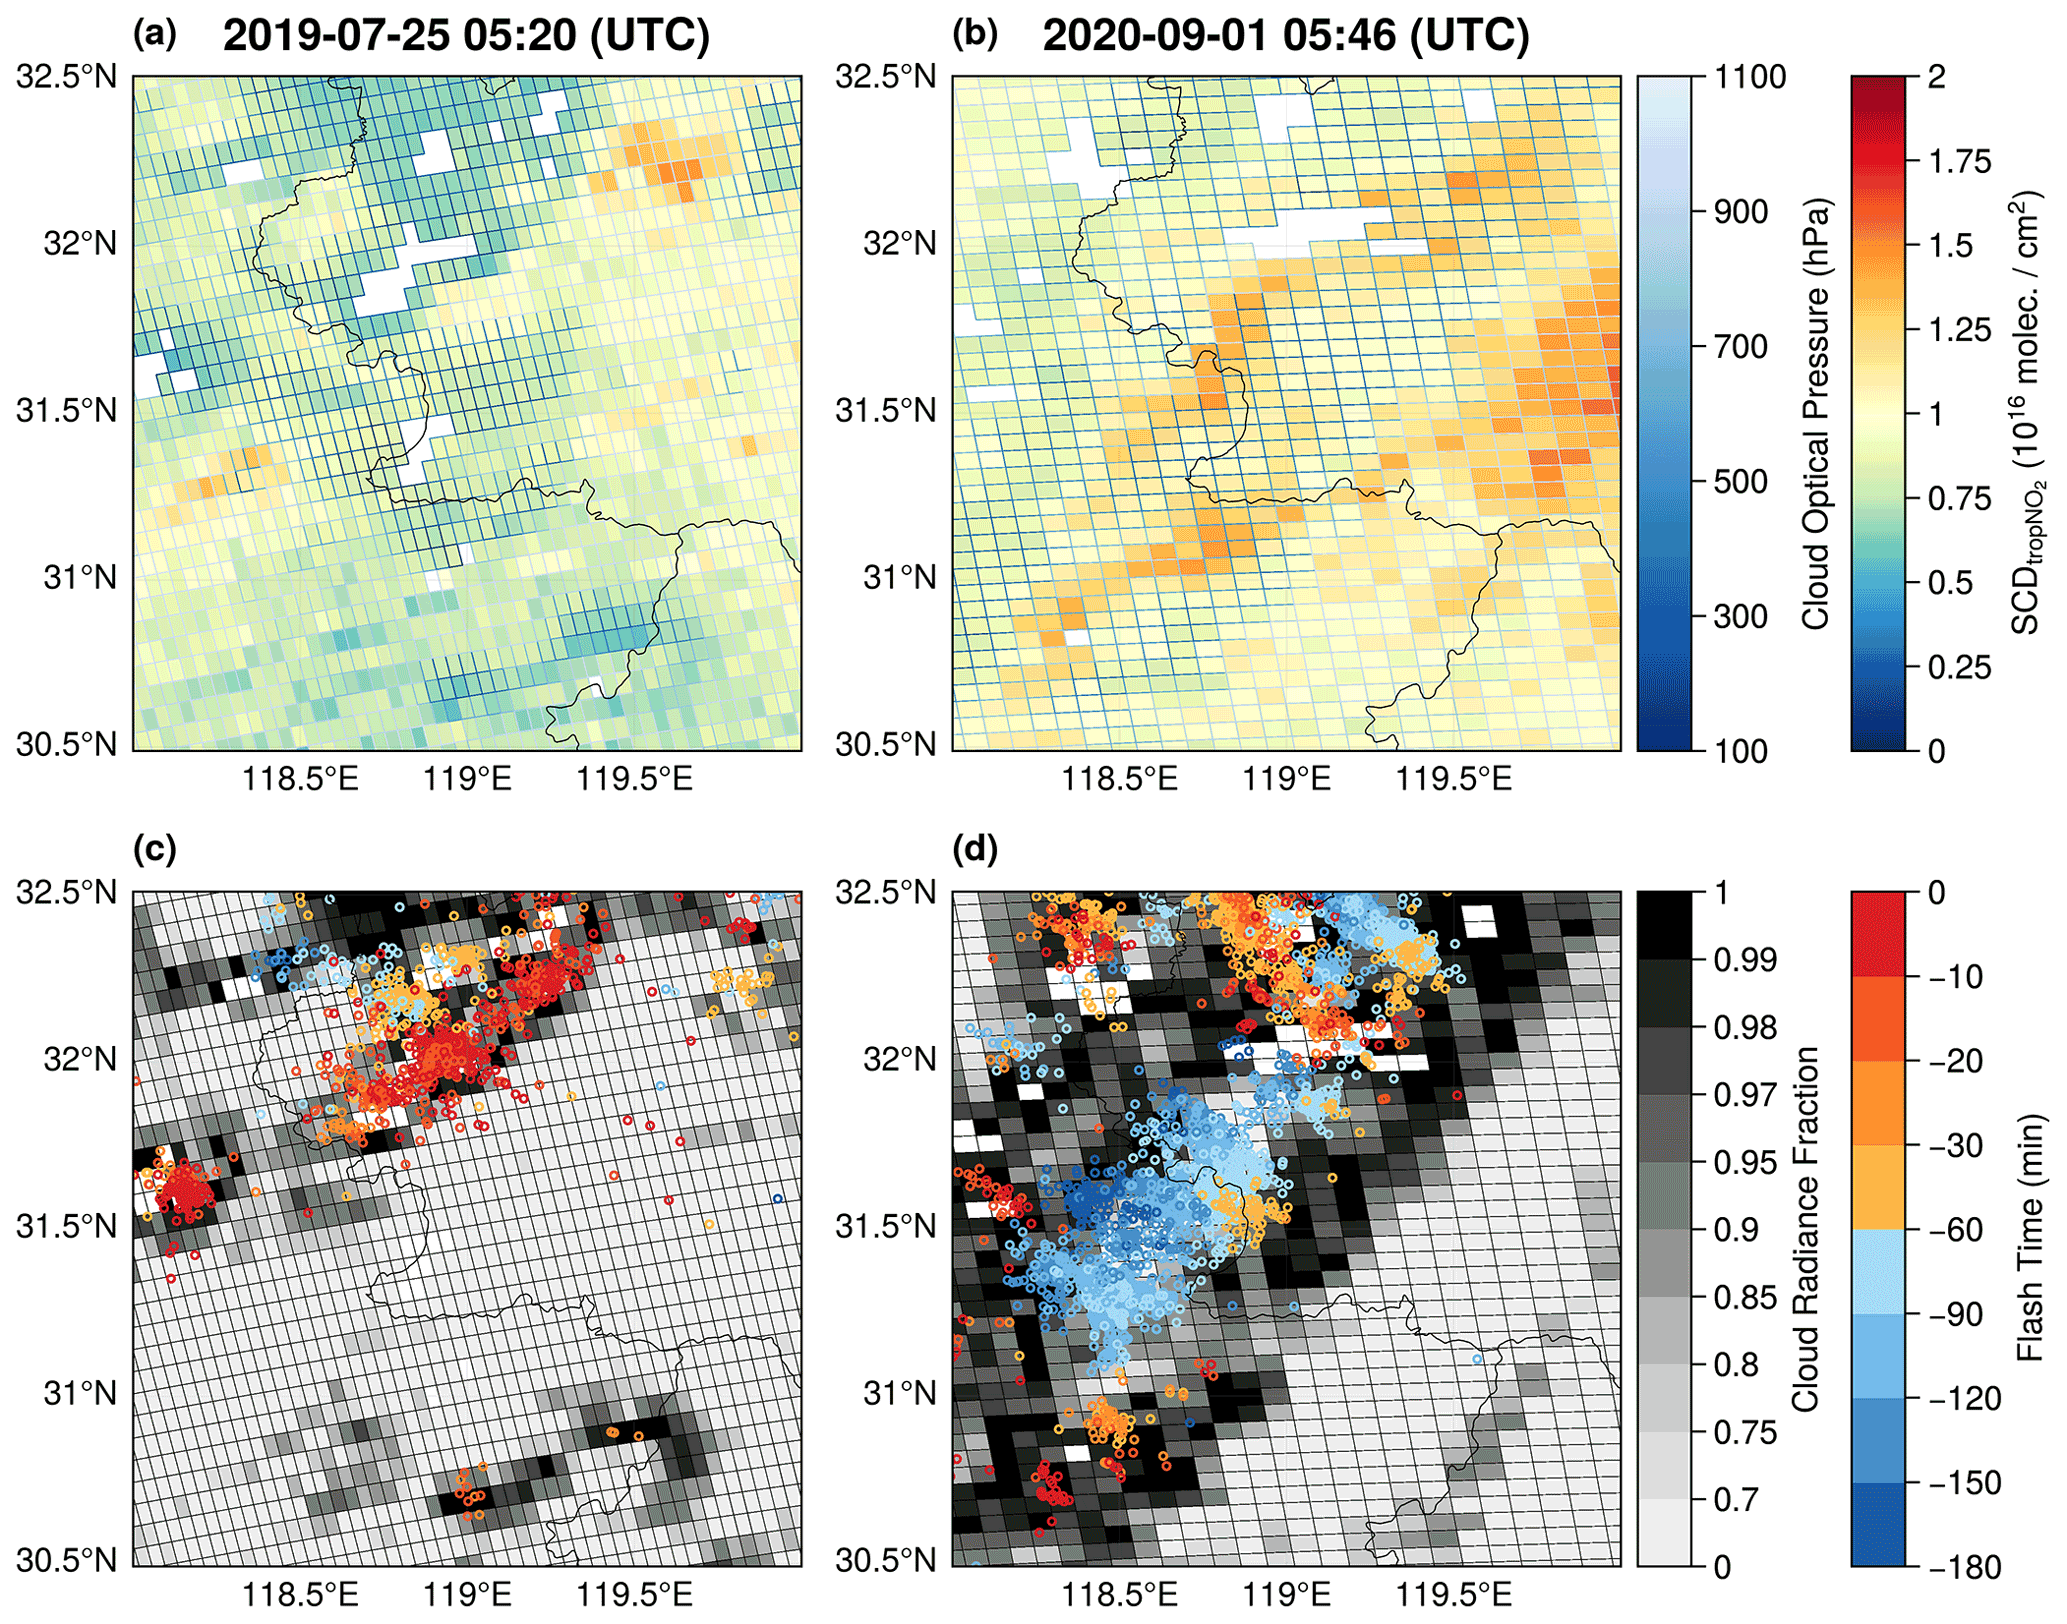
\includegraphics[width=\textwidth]{./figures/china_flash_scd.png}
    \caption{
    2019 年 7 月 25 日(左)和 2020 年 9 月 7 日(右)的对流个例。
    (a,b)对流层 NO$_{\ch{2}}$ 斜柱浓度($S_{\ch{NO2}}$,填充色)和云压(线条颜色)。
    白色网格代表缺失的 TROPOMI 数据,黑色实线为江苏省;
    (c,d)NO$_{\ch{2}}$ 窗区中的云辐射分数和闪电。闪电的颜色取决于相对于TROPOMI过境的发生时间。\\
    Figure \ref{fig:china_flash_scd}. Events on 25 July 2019 (left) and 07 September 2020 (right).
    (a, b) The tropospheric NO$_{\ch{2}}$ slant column density ($S_{\ch{NO2}}$, filled color) and cloud optical pressure (line color).
    These white grid cells stand for missing TROPOMI data.
    The solid black border is Jiangsu province.
    (c, d) The cloud radiance fraction in the NO$_{\ch{2}}$ window and flashes whose color depends on the occurring time relative to the TROPOMI overpass time.
    }
    \label{fig:china_flash_scd}
\end{figure}


在第\ref{chapter:retrieval}章和\ref{sec:china}节中,本研究利用对流旺盛时的卫星观测来估算 LNO$_{\ch{x}}$产率。
然而由于 TROPOMI 的像素饱和和对流区域的有限覆盖(图\ref{fig:china_flash_scd}c),
该方法难以用于范围小发展旺盛的对流(如2019年的个例)。
因此本节尝试不对云量加以限制,将该方法应用于消散期的对流(2020年个例,图\ref{fig:china_flash_scd}d)。
如图 \ref{fig:china_vcd_lnox}b--c 所示,闪电与TROPOMI的过境时间差大于 30 分钟但小于 3 小时。
由于 NO$_{\ch{2}}$ 的寿命在对流附近为 $\sim$ 3(2--12)小时 \citep{Nault.2016},
2020年个例的TROPOMI观测数据仍可以用于估算LNO$_{\ch{x}}$。
LNO$_{\ch{x}}$平均产率(mol/flash)的定义如下:
\begin{equation} \label{eq:lnox}
PE_{LNO_x} = \sum_{p} V_i A_i / \sum_{N} F_j e^{-(t_0 - t_j) / \tau}
\end{equation}
其中 $p$ 代表受 LNO$_{\ch{x}}$ 影响的像素,
$V_i$(mol/m$^2$)是像素 $i$ 上LNO$_{\ch{x}}$ 垂直柱浓度($V_{\ch{LNO_x}}$ = $S_{\ch{NO2}}$ / $AMF_{\ch{LNO_x}}$),
面积称为 A$_i$ (m$^2$),
$N$ 是 对 $V_{\ch{LNO_x}}$ 做出贡献的闪电总数,
指数部分考虑了每个闪电(F$_j$)排放的NO$_{\ch{x}}$ 的寿命。
具体而言,AMF$_{\ch{LNO_x}}$源于式(\ref{eq:AMF_LNO2}),
t$_0$是TROPOMI的过境时间,
t$_j$是闪电的发生时间,
$\tau$为近对流的NO$_{\ch{x}}$寿命(3 小时)。

由于消散的对流在旺盛期间已产生了足够多的闪电,
并且对流处对流层上层的风从西北偏西吹向东南偏东(图\ref{fig:china_vcd_lnox}a),
仍然可以清楚地识别出$V_{\ch{LNO_x}}$的范围(图\ref{fig:china_vcd_lnox} 中的虚线矩形),且有一条$V_{\ch{LNO_x}}$低值带将南北对流分开。
经过仔细选择,计算得到的LNO$_{\ch{x}}$产率为60 mol NO$_{\ch{x}}$每闪电。
虽然有些与 $V_{\ch{LNO_x}}$ 相关的闪电在选择的区域之外,
它对LNO$_{\ch{x}}$产率的影响仅 $\sim$ 2 mol,在下节的不确定性评估范围内。


% \begin{figure}[H]
%     \centering
%     
\includegraphics[width=\textwidth]{./figures/china_vcd_lnox.png}
%     \caption{
%     背景为LNO$_{\ch{x}}$垂直柱浓度($V_{\ch{LNO_x}}$)的分布。
%      白色矩形是为手动选择用于 LNO$_{\ch{x}}$产率估算的区域。
%      (a)中叠加的箭头是 WRF-Chem 模拟的 500 hPa 水平风;
%      (b)和(c)中的点是闪电,其颜色取决于相对于 TROPOMI 过境的发生时间。\\
%     Figure \ref{fig:china_vcd_lnox}. The background is the distribution of LNO$_{\ch{x}}$ vertical column densities ($V_{\ch{LNO_x}}$).
%     The white rectangles are manually selected regions for the LNO$_{\ch{x}}$ production efficiency estimation.
%     The overlayed wind arrows in (a) are the 500 hPa horizontal wind simulated by WRF-Chem.
%     The dots in (b) and (c) are the flashes whose color depends on the occurring time relative to the TROPOMI overpass time.
%     }
%     \label{fig:china_vcd_lnox}
% \end{figure}


根据 \citet{Allen.2019} 和 \citet{Zhang.2020b},LNO$_{\ch{x}}$ 的不确定性由 LNO$_{\ch{x}}$ 寿命、闪电探测效率、
NO/NO$_{\ch{2}}$ 比例、LNO 廓线和其他来源决定(表\ref{table:uncertainty_china})。
本研究将NO$_{\ch{2}}$的寿命替换为2 和6 h,得到的不确定性为27\%,而将IC与CG的比值改为2 :1 和 4:1,得到的不确定性也为27\%。
根据 \citet{Allen.2019} 本研究将由模拟引起的 NO/NO$_{\ch{2}}$ 比例的不确定性设置为 30\%,
此外利用330 和 700 mol NO每闪电的WRF-Chem敏感性试验结果,得到与LNO廓线有关的不确定性为 26\%。
与平流层垂直柱浓度[$\pm$ 10$^{14}$ molec. cm$^2$, \citet{VanGeffen.2022}]相关的不确定性为 7\%。
而由其他可能误差源引起的不确定性难以量化,比如斜柱浓度中的系统误差、云压和由对流重新分布的 NO$_{\ch{2}}$,
根据 \citet{Allen.2021a}本研究设其为10\%。
假设误差之间没有相关性,总不确定性(56\%)即为所有单个不确定性平方和的平方根。
因此LNO$_{\ch{x}}$产率为60 $\pm$ 33 mol NO$_{\ch{x}}$每闪电,
该数值低于第\ref{chapter:retrieval}章(90 $\pm$ 50 mol NO$_{\ch{x}}$每闪电)和\citet{Allen.2021a}(120 $\pm$ 65 mol NO$_{\ch{x}}$每闪电)在美国大陆的研究结果,
因此在未来的研究中还需对中国地区进行范围更广的探讨,
从而估算区域性的LNO$_{\ch{x}}$产率。


\begin{landscape}
\vspace*{\fill}
\begin{figure}[H]
    \centering
    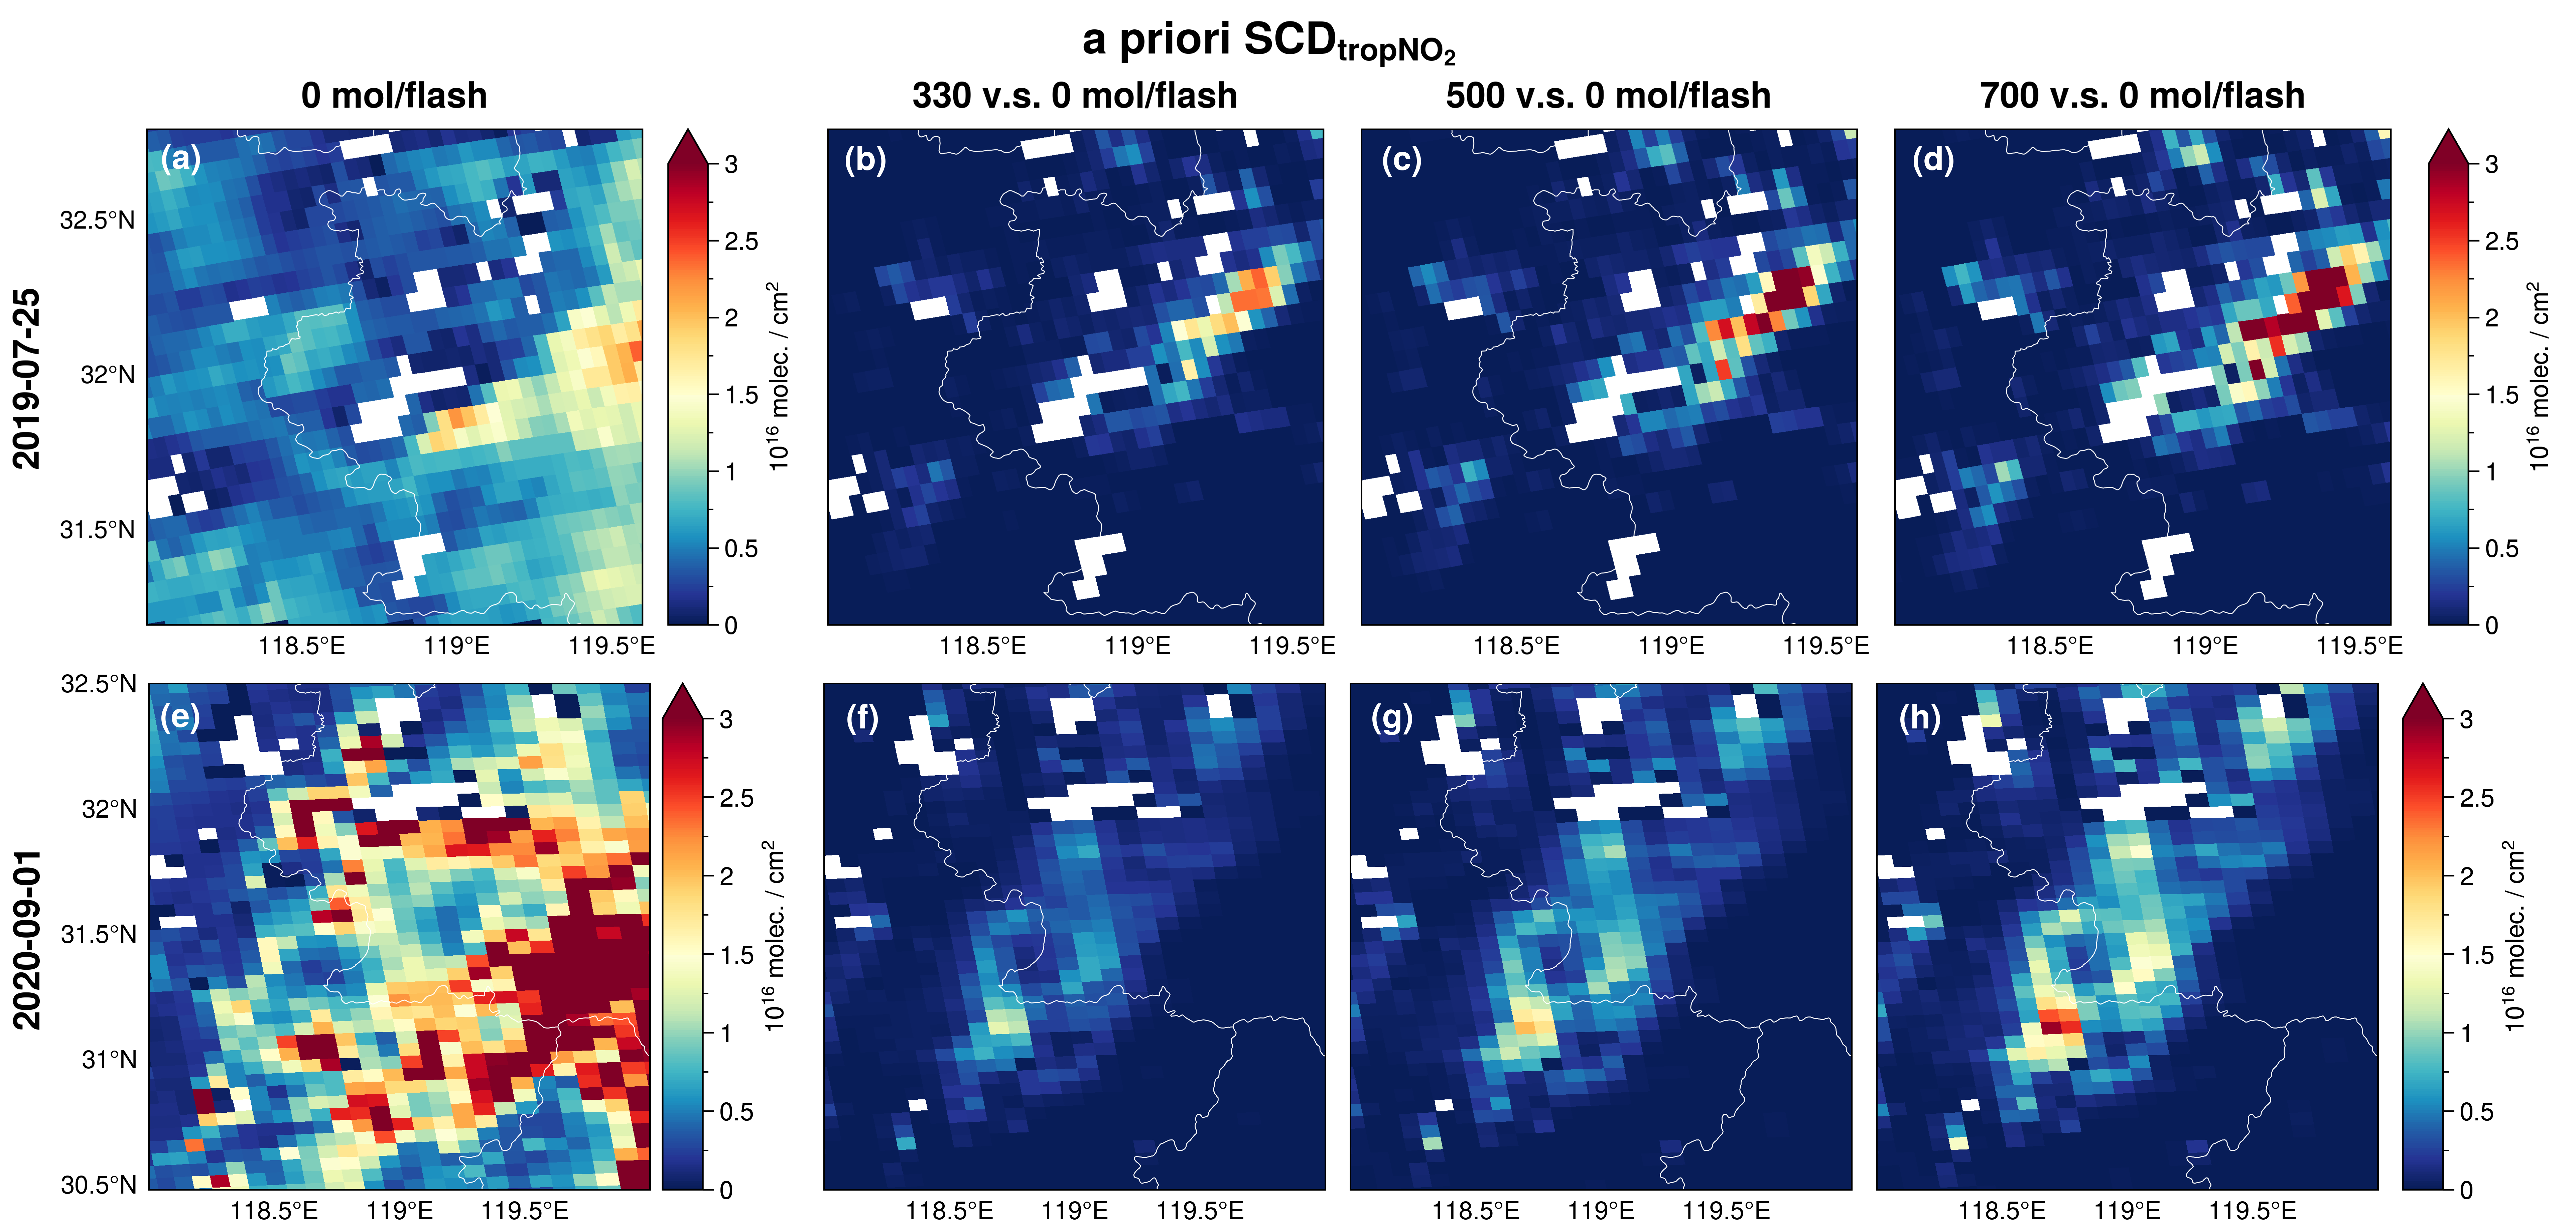
\includegraphics[width=0.9\columnwidth]{./figures/s5p_apriori_scd.png}
    \caption{使用不同闪电NO排放条件下WRF-Chem的NO$_{\ch{2}}$结果,重新计算得到的对流层NO$_{\ch{2}}$斜柱浓度($S_{\ch{NO2}}$)。
    (a,e)0 mol每闪电;(b,f)330 mol每闪电;(c,g)500 mol每闪电;(d,h)700 mol每闪电。\\
    Figure \ref{fig:s5p_apriori_scd}. The tropospheric NO$_{\ch{2}}$ slant column density ($S_{\ch{NO2}}$) recalculated using the WRF-Chem results with different lightning NO settings: (a, e) 0 mol/flash, (b, f) 330 mol/flash, (c, g) 500 mol/flash and (d, h) 700 mol/flash.
    }
    \label{fig:s5p_apriori_scd}
\end{figure}
\vspace*{\fill}
\end{landscape}

\begin{landscape}
\vspace*{\fill}
\begin{figure}[H]
    \centering
    
\includegraphics[width=0.9\columnwidth]{./figures/china_vcd_lnox.png}
    \caption{
    背景为LNO$_{\ch{x}}$垂直柱浓度($V_{\ch{LNO_x}}$)的分布。
     白色矩形是为手动选择用于 LNO$_{\ch{x}}$产率估算的区域。
     (a)中叠加的箭头是 WRF-Chem 模拟的 500 hPa 水平风;
     (b)和(c)中的点是闪电,其颜色取决于相对于 TROPOMI 过境的发生时间。\\
    Figure \ref{fig:china_vcd_lnox}. The background is the distribution of LNO$_{\ch{x}}$ vertical column densities ($V_{\ch{LNO_x}}$).
    The white rectangles are manually selected regions for the LNO$_{\ch{x}}$ production efficiency estimation.
    The overlayed wind arrows in (a) are the 500 hPa horizontal wind simulated by WRF-Chem.
    The dots in (b) and (c) are the flashes whose color depends on the occurring time relative to the TROPOMI overpass time.
    }
    \label{fig:china_vcd_lnox}
\end{figure}
\vspace*{\fill}
\end{landscape}
% \FloatBarrier

\begin{table}[H]
\footnotesize
\centering
\caption{LNO$_{\ch{x}}$产率估算的不确定性\\
Table \ref{table:uncertainty_china}. Uncertainties for the estimation of LNO$_\textrm{x}$ production efficiency.}
\begin{tabularx}{.8\textwidth}{c X}
\thickline
来源 & \makecell[cc]{不确定性 (\%)} \\
\thickline
LNO$_{\ch{x}}$ 寿命                & \makecell[cc]{27\%} \\
闪电探测效率                  & \makecell[cc]{27\%} \\
NO/NO$_{\ch{2}}$ 比例               & \makecell[cc]{30\%} \\
LNO 廓线                     & \makecell[cc]{26\%} \\
平流层垂直柱浓度                & \makecell[cc]{7\%} \\
其他                          & \makecell[cc]{10\%} \\
\hline
净不确定性                             & \makecell[cc]{56\%} \\
\thickline
\end{tabularx}
\label{table:uncertainty_china}
\end{table}


\subsection{闪电二氧化氮对TROPOMI二氧化氮产品的影响} \label{sec:lno2_affects_tropomi}

鉴于LNO$_{\ch{2}}$在对流层中上层的主导地位和更长寿命,TROPOMI的NO$_{\ch{2}}$产品可以用来研究不同区域LNO$_{\ch{2}}$的分布。
然而如上节所述,官方的TROPOMI NO$_{\ch{2}}$柱浓度产品所依赖的NO$_{\ch{2}}$先验廓线并未详细考虑LNO$_{\ch{2}}$的垂直分布,
所以本研究接着针对中国东部地区的对流系统,
利用WRF-Chem的敏感性试验结果,详细分析了LNO$_{\ch{x}}$对官方NO$_{\ch{2}}$柱浓度产品的影响。

为了探讨LNO$_{\ch{x}}$对AMF$_{\ch{trop}}$和AMF$_{\ch{LNO_x}}$计算的重要性,
本研究将LNO产率的上限700 mol NO 每闪电\citep{Ott.2010}应用于WRF-Chem ,并与500 mol NO 每闪电的结果进行对比。
接着通过独立替换对流层内三个不同高度区间的NO$_{\ch{2}}$廓线:
对流层中层(MT,800--400 hPa)、
对流层上层(UT,400--150 hPa)和整个对流层(地表到对流层顶),
进行TROPOMI AMF的敏感性试验。
除非另有说明,否则后文AMF的变化是通过增加LNO$_{\ch{x}}$获得。

如图\ref{fig:china_s5p_amf_diff}所示,
AMF变化主要由TROPOMI探测灵敏度高的对流层上层LNO$_{\ch{x}}$所控制\citep{Beirle.2009,Laughner.2017},
且LNO$_{\ch{x}}$产量在该高度达到峰值(图\ref{fig:china_nox_profile})。
虽然在三种廓线替换条件下AMF$_{\ch{LNO_x}}$均降低了5--40\%,
但AMF$_{\ch{trop}}$的变化($\Delta$AMF$_{\ch{trop}}$)具有区域特异性,
可根据闪电活动(图\ref{fig:china_flash_scd})对其进行分类:新生闪电区(MT $\Delta$AMF $<$ -20\%)、闪电下风向(MT $\Delta$AMF$_{\ch{trop}}$ $>$ 20\%)和闪电老化区(UT $\Delta$AMF$_{\ch{trop}}$ $>$ 20\%)。
结果表明,先验廓线中若考虑LNO$_{\ch{2}}$,可导致新生闪电区的AMF$_{\ch{trop}}$降低23\%,而闪电下风向和闪电老化区的AMF$_{\ch{trop}}$增大60\%。

接着本研究利用云高数据和敏感性试验结果,进一步分析了AMF$_{\ch{trop}}$在不同区域呈现不同变化的原因。
如图\ref{fig:china_amf_contribution}a所示,云层高于400 hPa时(云压 $<$ 400 hPa),
新生闪电区的像素上云辐射分数(f$_{\ch{effNO2}}$) $>$ 0.6,但闪电下风向和老化区均有低于400 hPa且f$_{\ch{effNO2}}$ $<$ 0.6的云层。
这与图\ref{fig:china_nox_profile}中的平均云压一致,并解释了为何UT $\Delta$AMF$_{\ch{trop}}$ > 20\% 在图\ref{fig:china_s5p_amf_diff}b$_i$和b$_{iii}$ 中存在,这也正表明了在闪电老化区估算LNO$_{\ch{x}}$的可能性。
具体而言,LNO$_{\ch{x}}$对$\Delta$AMF$_{\ch{trop}}$的贡献分为两部分:S$^{\ch{LNO_x}}_{\ch{tropNO2}}$/S$^{\ch{noLNO_x}}_{\ch{tropNO2}}$ 和 V$^{\ch{LNO_x}}_{\ch{tropNO2}}$/V$^{\ch{noLNO_x}}_{\ch{tropNO2}}$,
其中 LNO$_{\ch{x}}$ 上标表示先验变量是开启 LNO$_{\ch{x}}$排放(500 mol NO每闪电),而 noLNO$_{\ch{x}}$ 代表关闭LNO$_{\ch{x}}$排放。
这两个贡献是通过对式(\ref{eq:AMF1})和式(\ref{eq:AMF0})取对数,然后相减得到式(\ref{eq:delta_AMF}),其中下标$1$是开启LNO$_{\ch{x}}$排放,下标$0$是关闭LNO$_{\ch{x}}$排放。
这两部分可用于确定哪个参数控制$\Delta$AMF$_{\ch{trop}}$:增大的先验S$_{\ch{tropNO2}}$ 或先验 V$_{\ch{tropNO2}}$(图\ref{fig:china_amf_contribution}b--d)。
简而言之,图\ref{fig:china_amf_contribution}b--d中哪个比例的数值大,哪个占主导地位。
{
\abovedisplayskip=5pt%
\belowdisplayskip=5pt%
\begin{equation} \label{eq:AMF1}
\textrm{AMF}_1 = \frac{S_1}{V_1}
\end{equation}
\begin{equation} \label{eq:AMF0}
\textrm{AMF}_0 = \frac{S_0}{V_0}
\end{equation}
\begin{equation} \label{eq:delta_AMF}
\begin{split}
\textrm{log(AMF$_1$)} - \textrm{log(AMF$_0$)} & = \textrm{log}(\frac{S_1}{V_1}) - \textrm{log}(\frac{S_0}{V_0}) \\
                                              & = \textrm{log}(\frac{S_1}{S_0}) - \textrm{log}(\frac{V_1}{V_0})
\end{split}
\end{equation}
}

首先,如果将LNO$_{\ch{2}}$包含在先验NO$_{\ch{2}}$廓线中(图\ref{fig:china_s5p_amf_diff}c$_i$),
新生闪电区由于增大的先验V$_{\ch{NO2}}$(图 \ref{fig:china_amf_contribution}b),AMF$_{\ch{trop}}$将减小。
而新生闪电的下风向区域情况相反,无论选择哪一层替换NO$_{\ch{2}}$廓线,
AMF$_{\ch{trop}}$均增大(图\ref{fig:china_s5p_amf_diff}a$_{i}$--c$_{i}$),
这是由于对流将LNO$_{\ch{2}}$输送至云顶上方,并导致更大的先验 S$_{\ch{NO2}}$(图 \ref{fig:china_amf_contribution}c)。
对于2020年个例的老化闪电像素处,针对对流层上层的AMF$_{\ch{trop}}$结果增加$>$50 \%(图\ref{fig:china_s5p_amf_diff}b$_{iii}$)。
该现象证明了云作为屏障和平流输送的对流层上层LNO$_{\ch{2}}$的重要作用,即导致先验S$_{\ch{NO$_2$}}$和先验V$_{\ch{NO2}}$之间的差异(图 \ref{fig:china_amf_contribution}d)。
尽管由于对流附近LNO$_{\ch{2}}$的寿命较短,该差异小于其他两个区域,但它对于计算LNO$_{\ch{x}}$ 仍然有用。
此外,考虑到LNO$_{\ch{x}}$对AMF影响的区域性,TROPOMI的NO$_{\ch{2}}$ 的产品需更为详细地考虑LNO$_{\ch{2}}$,尤其是在出流区域。
而TM5 和 WRF-Chem NO$_{\ch{2}}$ 廓线之间的比较(图 \ref{fig:china_nox_profile})也说明了可分辨的对流输送和LNO$_{\ch{x}}$的重要性。


\begin{figure}[H]
    \centering
    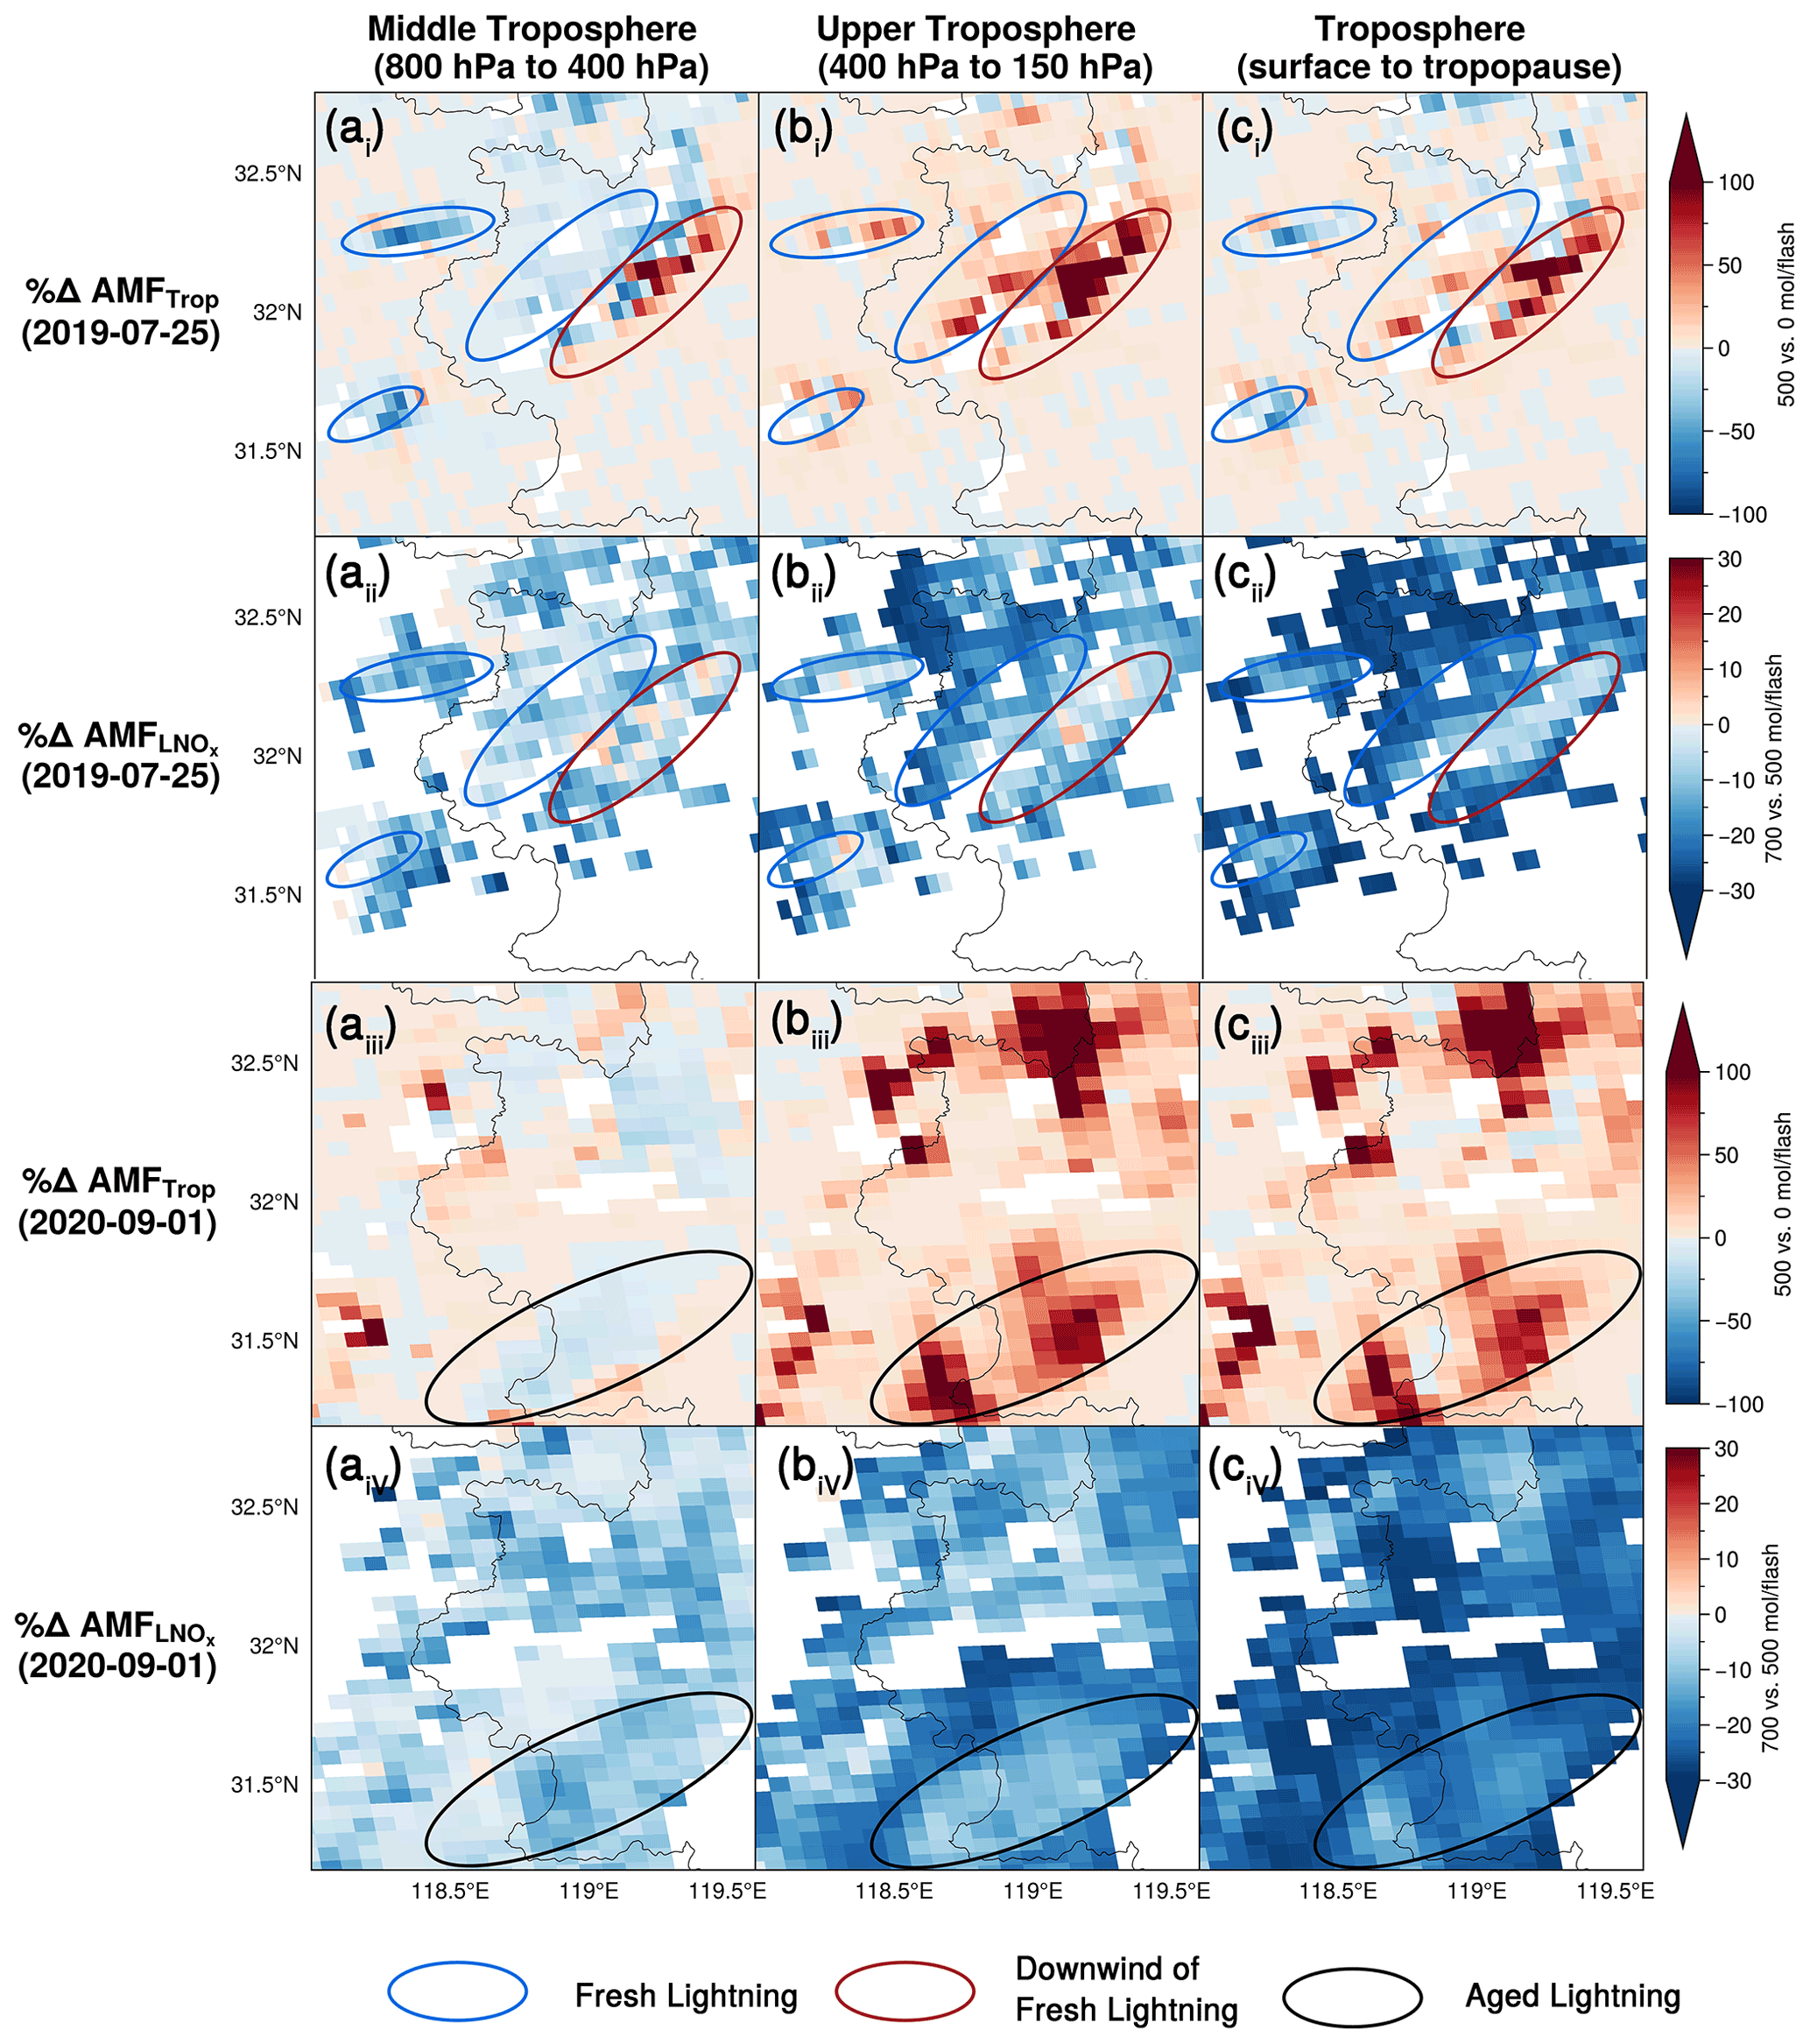
\includegraphics[width=0.9\textwidth]{./figures/china_s5p_amf_diff.png}
    \caption{
    通过替换三层的NO$_{\ch{2}}$先验廓线,得到的大气质量因子(AMF)百分比差异。
    三层具体为:对流层中层(左)、对流层上层(中)和整个对流层(右)。
     $\Delta$AMF$_\textrm{trop}$ 是 500 mol NO每闪电得到的AMF$_\textrm{trop}$ 与 0 mol NO每闪电得到的AMF$_\textrm{trop}$之差。
     $\Delta$AMF$_\textrm{LNO$_{\ch{x}}$}$ 是 700 mol NO每闪电得到的AMF$_\textrm{LNO$_{\ch{x}}$}$ 与 500 mol NO每闪电得到的AMF$_\textrm{LNO$_{\ch{x}}$}$之差。
     图中标注的三个椭圆区域为:新生闪电区(蓝色),闪电下风向(红色),和闪电老化区(黑色)。\\
    Figure \ref{fig:china_s5p_amf_diff}. The percent differences of AMFs by replacing the a priori NO$_{\ch{2}}$ profiles at three layers:
    middle troposphere (left), upper troposphere (middle), and troposphere (right).
    $\Delta$AMF$_\textrm{trop}$ is the comparison of the AMF$_\textrm{trop}$ with 500 mol NO per flash relative to 0 mol NO per flash.
    $\Delta$AMF$_\textrm{LNO$_{\ch{x}}$}$ is the comparison of the AMF$_\textrm{LNO$_{\ch{x}}$}$ with 700 mol NO per flash relative to 500 mol NO per flash.
    Three regions are annotated: fresh lightning (blue),
    downwind of fresh lightning (red),
    and aged lightning (black).
    }
    \label{fig:china_s5p_amf_diff}
\end{figure}


\begin{landscape}
\vspace*{\fill}
\begin{figure}[H]
    \centering
    \makebox[0pt]{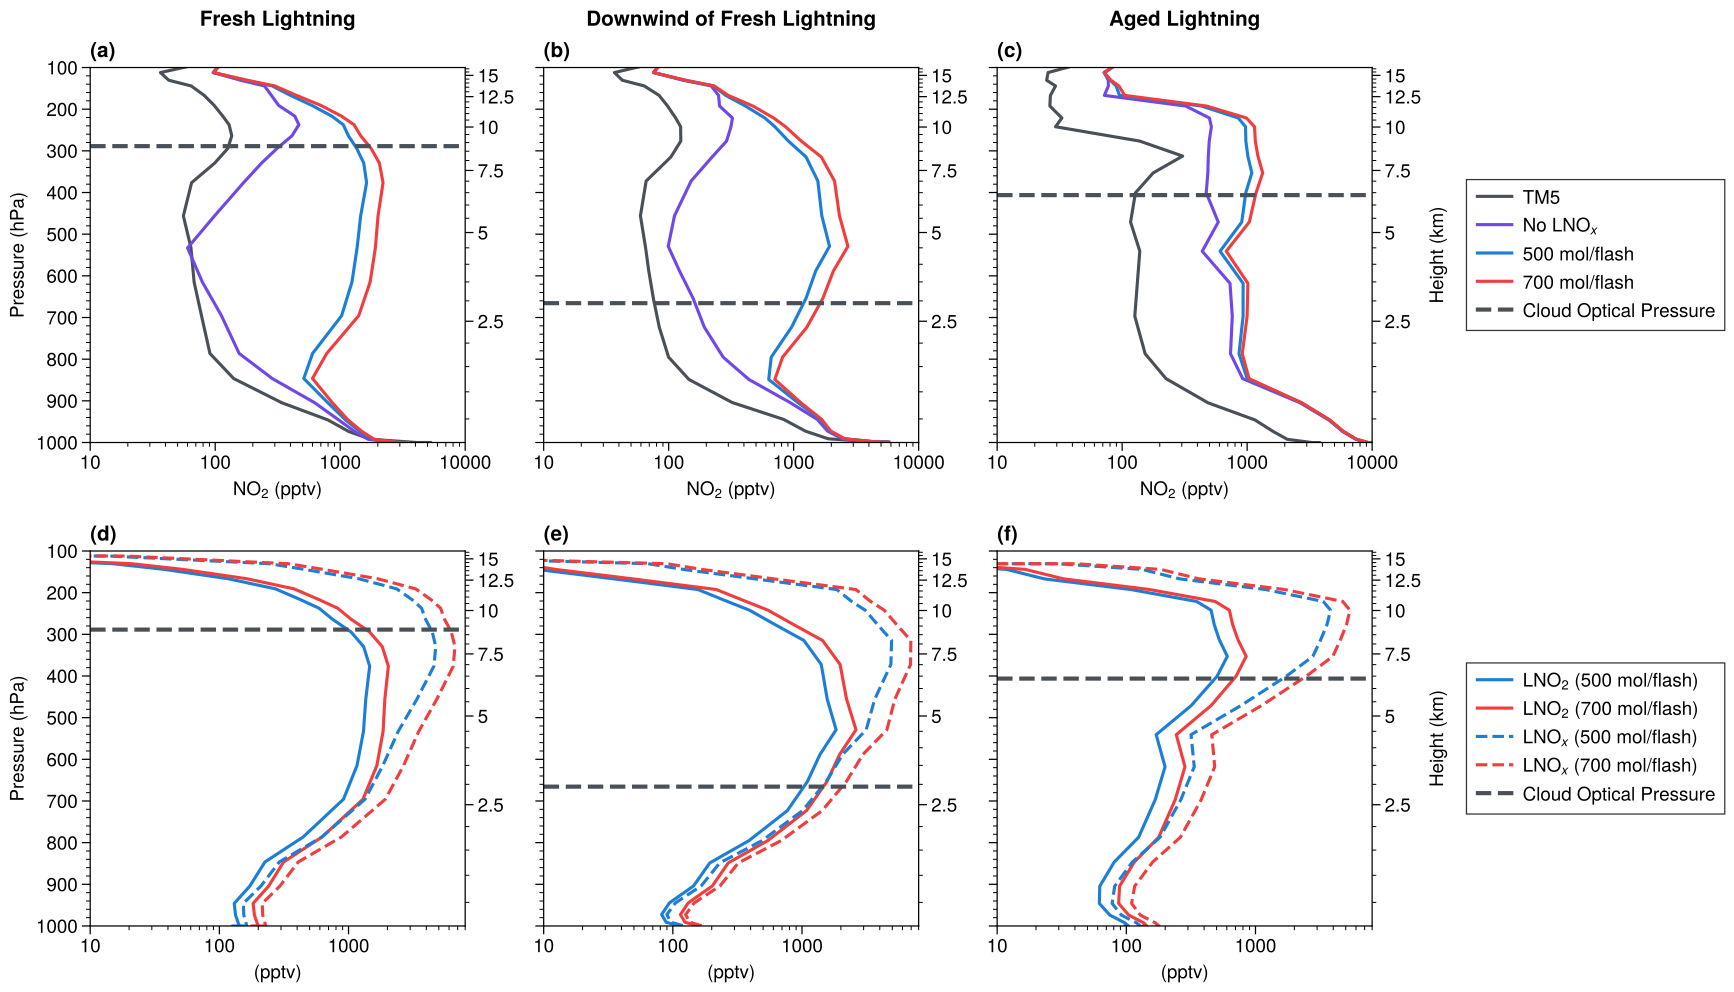
\includegraphics[width=0.76\columnwidth]{./figures/china_nox_profile.png}}
    \caption{
    TROPOMI过境时在不同闪电NO的排放条件下,三个区域(新生闪电区、闪电下风向和闪电老化区)的各物质垂直廓线。
    (a--c)NO$_{\ch{2}}$廓线与官方TM5先验NO$_{\ch{2}}$廓线之间的比较。
    (d--f)在不同闪电NO产率设置的条件下,LNO$_{\ch{2}}$ 和 LNO$_{\ch{x}}$之间的廓线分布比较。灰色虚线是TROPOMI探测到的云压。\\
     Figure \ref{fig:china_nox_profile}. Profiles with different lightning NO productions at TROPOMI overpass time over three regions (fresh lightning, downwind of fresh lightning, and aged lightning).
    (a--c) The NO$_{\ch{2}}$ profiles compared with the official TM5 a priori NO$_{\ch{2}}$ profile.
    (d--f) The comparisons between LNO$_{\ch{2}}$ and LNO$_{\ch{x}}$ profiles with different lightning NO production settings.
    The gray dashed line is the cloud optical pressure detected by TROPOMI.
    }
    \label{fig:china_nox_profile}
\end{figure}
\vspace*{\fill}
\end{landscape}


\begin{figure}[H]
    \centering
    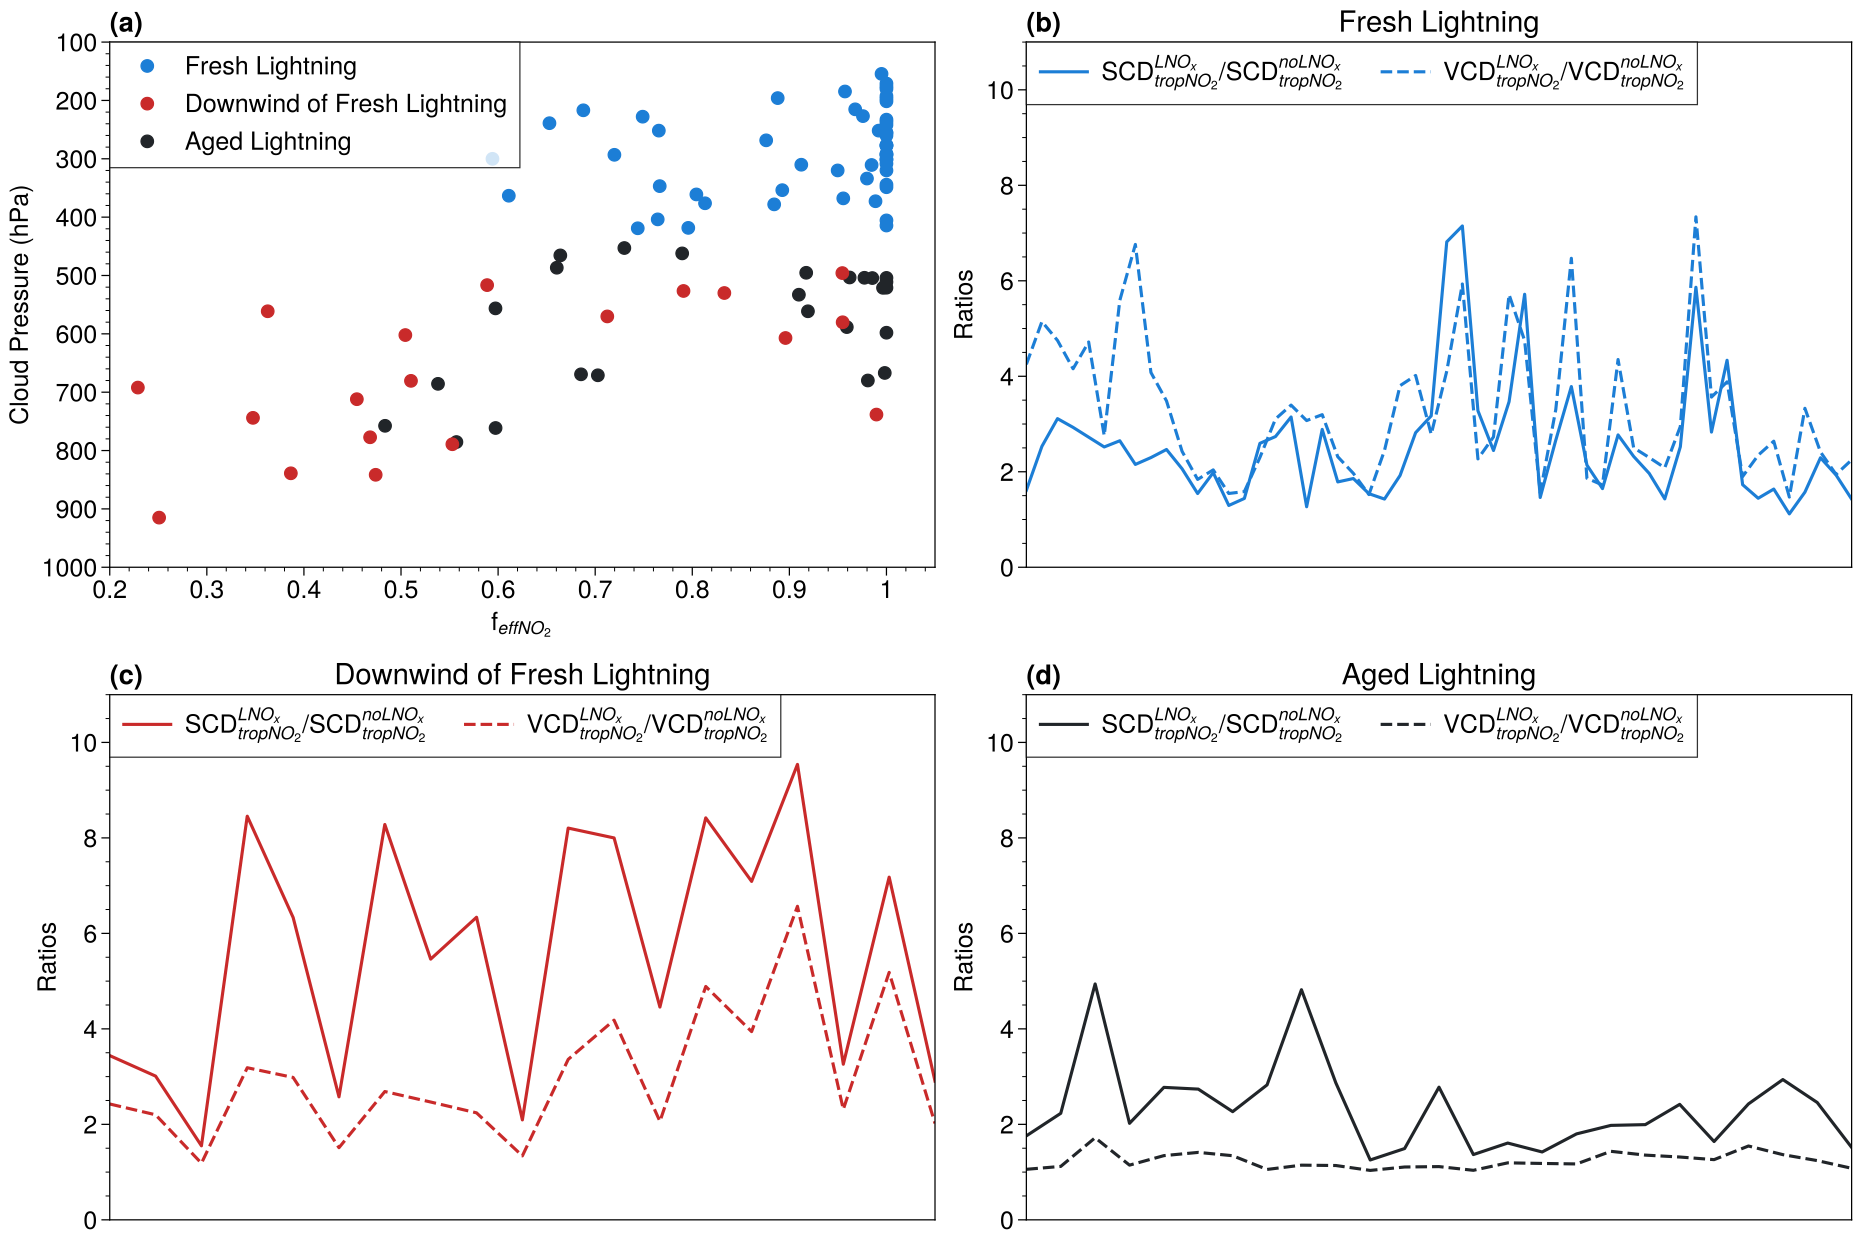
\includegraphics[width=\textwidth]{./figures/china_amf_contribution.png}
    \caption{
    (a)图 \ref{fig:china_s5p_amf_diff} 中定义的三个区域(新生闪电区,闪电下风向,和闪电老化区)的云压和云辐射分数之间的关系。
     (b--d)这三个区域的先验SCD$^{\textrm{LNO$_{\ch{x}}$}}_{\textrm{tropNO$_{\ch{2}}$}}$/SCD$^{\textrm{noLNO$_{\ch{x}}$}}_{ \textrm{tropNO$_{\ch{2}}$}}$和先验VCD$^{\textrm{LNO$_{\ch{x}}$}}_{\textrm{tropNO$_{\ch{2}}$}}$/VCD$^{\textrm{noLNO$_{\ch{x}}$ }}_{\textrm{tropNO$_{\ch{2}}$}}$。
     LNO$_{\ch{x}}$的上标表示先验变量是通过开启LNO$_{\ch{x}}$排放(500 mol NO每闪电),而上标为noLNO$_{\ch{x}}$代表关闭LNO$_{\ch{x}}$排放。\\
     Figure \ref{fig:china_amf_contribution}. (a) The relationship between cloud pressure and cloud radiance fraction for three regions defined in Fig. \ref{fig:china_s5p_amf_diff}: fresh lightning region, downwind of fresh lightning, and aged lightning area.
    (b--d) The a priori SCD$^{\textrm{LNO$_{\ch{x}}$}}_{\textrm{tropNO$_{\ch{2}}$}}$/SCD$^{\textrm{noLNO$_{\ch{x}}$}}_{\textrm{tropNO$_{\ch{2}}$}}$ and a priori VCD$^{\textrm{LNO$_{\ch{x}}$}}_{\textrm{tropNO$_{\ch{2}}$}}$/VCD$^{\textrm{noLNO$_{\ch{x}}$}}_{\textrm{tropNO$_{\ch{2}}$}}$ of pixels in these three regions. The LNO$_{\ch{x}}$ superscript indicates that the a priori variable is calculated with LNO$_{\ch{x}}$ (500 mol NO per flash) and the noLNO$_{\ch{x}}$ superscript is without LNO$_{\ch{x}}$.
    }
    \label{fig:china_amf_contribution}
\end{figure}



\section{清洁地区(北极)} \label{sec:arctic}

\subsection{闪电的分布} \label{subsect:lightning_distribution}

全球气候变暖正在引起闪电分布的变化\citep{Reeve.1999,Williams.2005a,Price.2009a}。
在过去的 30 年中,研究学者针对闪电预测提出了多种模拟方案\citep{Price.1992,Price.1997b,Allen.2002,Futyan.2007,Finney.2014,Romps.2014}。
气候模式模拟结果显示,中纬度地区的闪电将有所增加\citep{Michalon.1999,Romps.2014,Luhar.2021},
而在热带地区不同方案的预测结果目前仍存在分歧\citep{Finney.2018,Romps.2019}。
此外,虽然北极地区变暖速度是全球平均水平的4倍\citep{Rantanen.2022},但针对北极闪电的研究还很少。
最近,\citet{Chen.2021a}针对北极地区开发了闪电参数化方案,
结果表明,若本世纪末全球平均气温上升3.7 $^{\circ}$C,永冻区的闪电频率将增加74--150\%。
地基闪电观测结果显示,北极闪电相对于全球闪电的比例在2010至2020年期间增加了两倍\citep{Holzworth.2021}。
此外,北极地区在夏季将有更多的水汽辐合来加强对流系统,从而导致更多的闪电\citep{Bintanja.2020}。

为了研究北极地区的闪电变化,本研究将光学瞬态探测器(OTD,1996--1999)的卫星闪电数据
与维萨拉全球地基雷电数据集(GLD360,2019--2021)进行比较。
其中OTD的数据产品为闪电次数,一次闪电可包含一个或多个闪击。
虽然GLD360官方产品只包含闪击,但是本研究的目的是研究闪电分布的变化,故未将闪击聚类成闪电。
GLD360数据覆盖了整个高纬度地区($>$60$^{\circ}$ N),而OTD仪器只观测75$^{\circ}$ N以南的闪电。
在2019--2021年夏季(6月至8月)GLD360探测到75$^{\circ}$ N 以北发生的闪击所占比例为3\%(图\ref{fig:gld360_tseries})。

\begin{figure}[H]
\centering
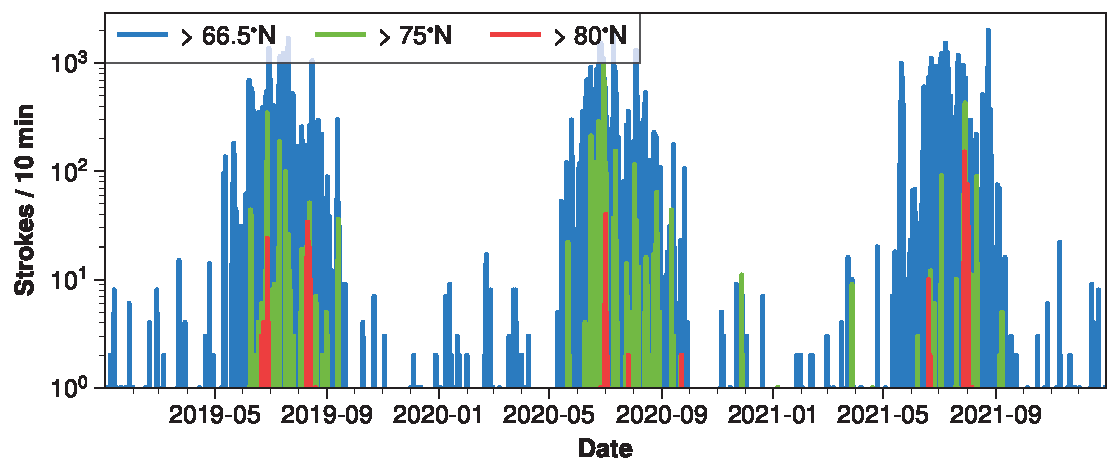
\includegraphics[width=0.9\textwidth]{./figures/arctic_gld360_tseries.png}
\caption{
GLD360探测的每10分钟闪击时间序列。\\
Figure \ref{fig:gld360_tseries}. Time series of GLD360 lightning strokes per 10 minutes.
}
\label{fig:gld360_tseries}
\end{figure}


图\ref{fig:arctic_lightning_distribution}比较了卫星和地基闪电网在高纬度地区观测到的夏季闪电空间分布。
两个数据集均显示北极野火的主要发生地[西伯利亚和阿拉斯加永冻区,
\citep{McCarty.2021}]具有较高的闪电频率(图\ref{fig:arctic_lightning_distribution}a,b)。
OTD测得的平均闪电频率和GLD360测得的平均闪击频率分别为0.22 km$^{-2}$每月和0.61 km$^{-2}$每月。
然而,OTD 在楚科奇海(Chukchi Sea)附近记录的闪电较少,但在伊明格海(Irminger Sea)上空较多。
该现象与北极降水的年际变化和向极地输送的水汽有关\citep{Bintanja.2020}。

为了判断 TROPOMI 是否可以探测到 LNO$_{\ch{2}}$,本研究首先计算了每次TROPOMI过境前3 h内条带内发生的GLD360闪击数。
由于TROPOMI在北极地区每天有14条重叠条带,条带内的闪击数约占总数的 9\%(图\ref{fig:arctic_lightning_distribution}c),并且具有相同的地理分布(图\ref{fig:arctic_lightning_distribution}b)。
纬度越高,条带内闪击的占比越大(图\ref{fig:arctic_lightning_distribution}d),
从$<$ 10\%(60--70$^{\circ}$ N)增加到 10--25\%(70--80$^{\circ}$ N)和40--100\%(80--90$^{\circ}$ N)。
由于地基观测\citep{Schmale.2018} 和飞机观测\citep{Jacob.2010}的NO$_{\ch{2}}$数据有限,
TROPOMI的观测数据在分析北极地区的 LNO$_{\ch{2}}$ 方面十分有利。
鉴于 70$^{\circ}$ N 以北具有更高的 TROPOMI 覆盖率和更少的其他NO$_{\ch{2}}$排放源(例如野火或天然气),本研究选择该区域来计算LNO$_{\ch{2}}$ 产率。
如表\ref{table:arctic_emission}所示,GLD360在70$^{\circ}$ N 以北探测到的夏季闪击数分别为 1.2$\times$10$^6$ (2019)、1.6$\times$10$^6$ (2020) 和 9.8$\times$10$^5$ ( 2021)。
其中在TROPOMI 覆盖率最高的地区(80--90$^{\circ}$ N),2021 年的闪击数约为 2.9$\times$10$^4$,是前九年总数的近两倍\citep{networktotal.2021}。
GLD360测得的闪击最北可达89.5$^{\circ}$ N,WWLLN也探测到了该次闪击[89.6 $^{\circ}$ N,\citet{Holzworth.2021}]。

\subsection{闪电二氧化氮的计算} \label{sec:arctic_lnox_calc}

LNO$_{\ch{2}}$的估算包括以下三个主要步骤:

(1) 使用风场数据将NO$_{\ch{2}}$柱浓度高值区与闪电数据匹配。

(2) 基于新算法来计算LNO$_{\ch{2}}$柱浓度。

(3) 使用连续的TROPOMI观测数据来计算LNO$_{\ch{2}}$的产率。

\begin{table}[H]
\centering
\caption{2019至2021年6--8月北极地区GLD360探测到的闪击数、闪电NO$_{\ch{2}}$排放(吨氮)和平均对流有效位能(CAPE,J kg$^{-1}$)\\
Table \ref{table:arctic_emission}. GLD360 stroke counts, lightning NO$_{\ch{2}}$ (LNO$_{\ch{2}}$) emissions (Mg of N), and mean
convective available potential energy (CAPE, J kg$^{-1}$) in the Arctic region during June--August 2019--2021.
}
\label{table:arctic_emission}
\footnotesize
% \renewcommand{\arraystretch}{0.6}
\begin{tabular}{llllll}
\thickline
{} & 70--75$^{\circ}$ N & 75--80$^{\circ}$ N &
80--85$^{\circ}$ N &  85--90$^{\circ}$ N &  \\
\thickline
闪击 & & & & & 总数 \\
\hline
2019 &   1,142,292 &     40,660 &      5,756 &       636  & 1,189,344 \\
2020 &   1,402,304 &    233,780 &      4,784 &       768  &  1,641,636 \\
2021 &     889,248 &     62,296 &     26,576 &      2,536  &  980,656 \\
\hline
闪电NO$_{\ch{2}}$排放 & & & & & 总数 \\
\hline
2019 &      87.3 &       5.6 &       0.9 &       0.1 &   93.9 \\
2020 &      85.5 &      22.1 &       0.8 &       0.1 &  108.5 \\
2021 &      58.6 &       8.6 &       3.9 &       0.4 &   71.5 \\
\hline
对流有效位能 & & & & & 平均值 \\
\hline
2019 & 5.5  & 4.0  & 5.0  & 6.5 & 5.3 \\
2020 & 9.2  & 5.1  & 5.0  & 5.2 & 6.1 \\
2021 & 7.3  & 4.8  & 5.5  & 7.2 & 6.2 \\
\thickline
\end{tabular}
\end{table}


\clearpage\vspace*{\fill}
\begin{figure}[H]
\centering
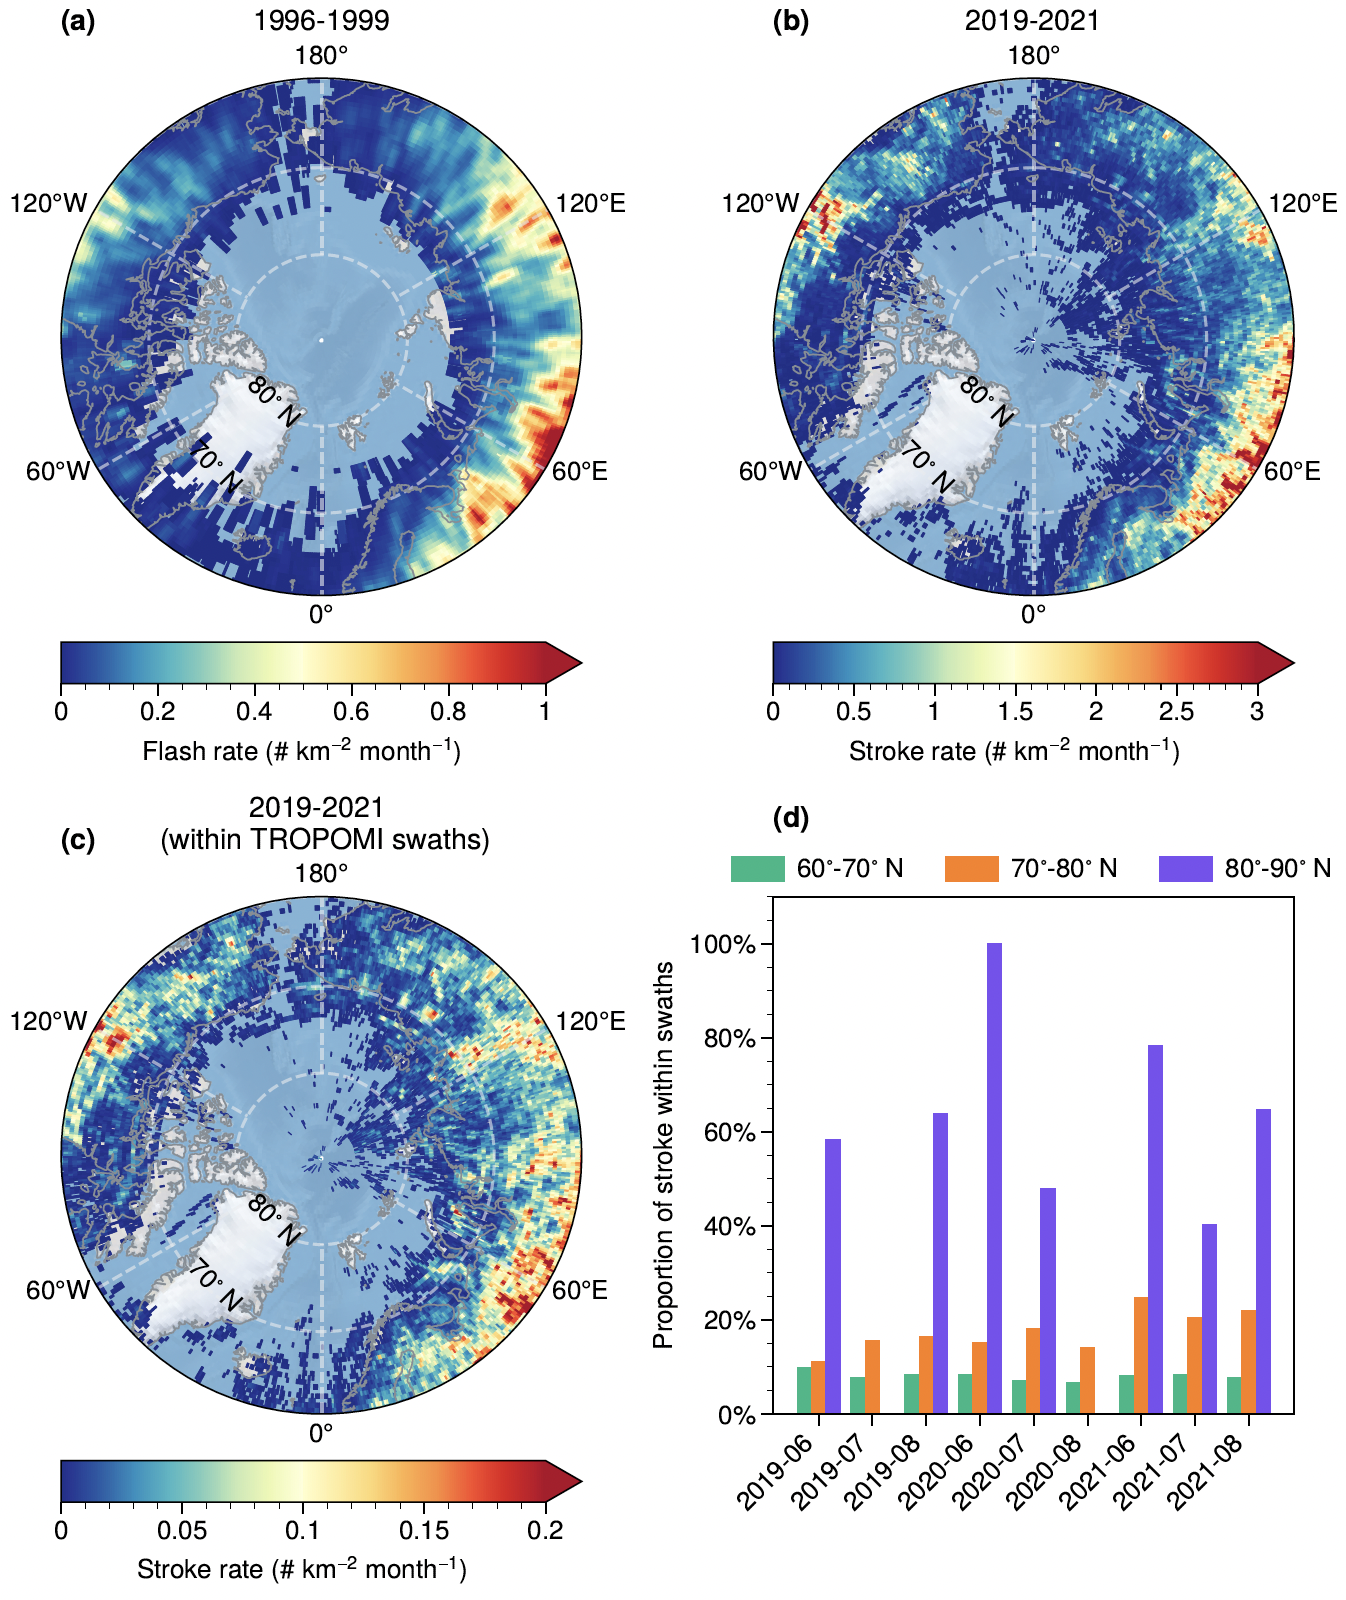
\includegraphics[width=0.9\textwidth]{./figures/arctic_lightning_distribution.png}
\caption{
(a)1996至1999年6-8月OTD观测的平均闪电频率;
(b)2019至2021年6-8月GLD360观测的平均闪击频率;
(c)与(b)相同,但只计算TROPOMI过境前3 h内TROPOMI条带内的闪电;
(d)为(c)与(b)的月比例。\\
Figure \ref{fig:arctic_lightning_distribution}.
(a) Mean OTD lightning flash rate of June--August 1996--1999;
(b) Mean GLD360 lightning stroke rate of June--August 2019--2021;
(c) Same as panel b but only counting the lightning inside the TROPOMI swaths during the 3 h period before the TROPOMI overpass time.
Grids with no lightning appear as the light-blue backgrounds in panels a--c.
(d) Monthly ratio of panel c to panel b.
}
\label{fig:arctic_lightning_distribution}
\end{figure}
\vspace*{\fill}\clearpage

\subsection*{闪电的聚类}

本研究使用密度聚类算法(DBSCAN)将TROPOMI过境前12 h内\citep{Allen.2021a}的闪击以40 km进行聚类\citep{backlund2011density,Schubert.2017}。
由于野火也会产生 NO$_{\ch{2}}$,因此使用可见光/红外成像仪/辐射计套件(VIIRS)375 m 主动火点产品,
来识别和过滤受野火排放影响的闪电聚类。
VIIRS 搭载在 Suomi 国家极地轨道合作伙伴 (Suomi-NPP)上,
它与搭载TROPOMI的S5P位于同一轨道,但比 S5P 提前3.5分钟。
本研究将内部没有火点的闪电集群视为一个清洁的聚类。

对于每个清洁的闪电聚类,本研究根据观测到的闪击所处位置及发生时间,
在三个气压层(300、500和700 hPa)上定义受 LNO$_{\ch{2}}$ 影响的空气块(图 \ref{fig:workflow}a)。
如图 \ref{fig:workflow}b 所示,本研究使用 ECMWF 小时大气再分析资料(ERA5) 的风场数据\citep{Hersbach.2020},
对含LNO$_{\ch{2}}$ 的空气块进行水平平流输送,并得到TROPOMI 过境时空气块的位置。
最终所有的空气块组成一个闪电掩膜(图 \ref{fig:workflow}c中的橙色圆圈),即三个等压面的前向轨迹构成了一个近似的 LNO$_{\ch{2}}$ 区域。

本研究首先使用分水岭方法得到对流层NO$_{\ch{2}}$垂直柱浓度($V_{\ch{NO2}}$)的高值区(图 \ref{fig:workflow}c中的像素)。
具体而言,分水岭方法将输入数据视为地形表面,并将它们分成单独的区域,称为集水盆地\citep{Soille.1990,Heikenfeld.2019a}。
本研究应用从 4$\times$10$^{14}$ 到 1$\times$10$^{15}$ molec. cm$^{-2}$ 的阈值,步长为 2$\times$10$^{14}$ molec. cm$^{-2}$来检测多个局部NO$_{\ch{2}}$高值特征。
这些特征用于识别具有高 $V_{\ch{NO2}}$ 的附近区域(图 \ref{fig:workflow}c 中不同颜色的像素)。
接着选择包含一个或多个高 $V_{\ch{NO2}}$ 区域的掩膜用于 LNO$_{\ch{2}}$ 的进一步分析,
最终对闪电掩膜内的数据用分水岭方法进行重新识别,得到具有高$V_{\ch{NO2}}$的LNO$_{\ch{2}}$ 区域(图 \ref{fig:workflow}d 中的亮色像素)。

在重新使用分水岭方法之前,本研究使用最小--最大归一化将掩膜内的 $V_{\ch{NO2}}$ 值归一化为 0--1 的范围,即从每个数据中减去最小值并除以最大值和最小值之间的差值。
本研究将对数正态分布模型拟合到置信度为 80\% 的归一化值,并将结果用作分水岭过程的最小阈值。
由于 LNO$_{\ch{2}}$ 区域通常小于闪电掩模(图 \ref{fig:workflow}d),
80\% 的置信水平应足以识别 LNO$_{\ch{2}}$ 像素,
与置信度相关的不确定性见表 \ref{table:arctic_uncertainty}。
最后,本研究将分水岭算法应用于标准化的 $V_{\ch{NO2}}$ 值,使用的阈值范围从最小值到 1,步长为 10,
从而识别和分析最终的LNO$_{\ch{2}}$数据(图 \ref{fig:workflow}d中亮色像素)。


\begin{figure}[H]
\centering
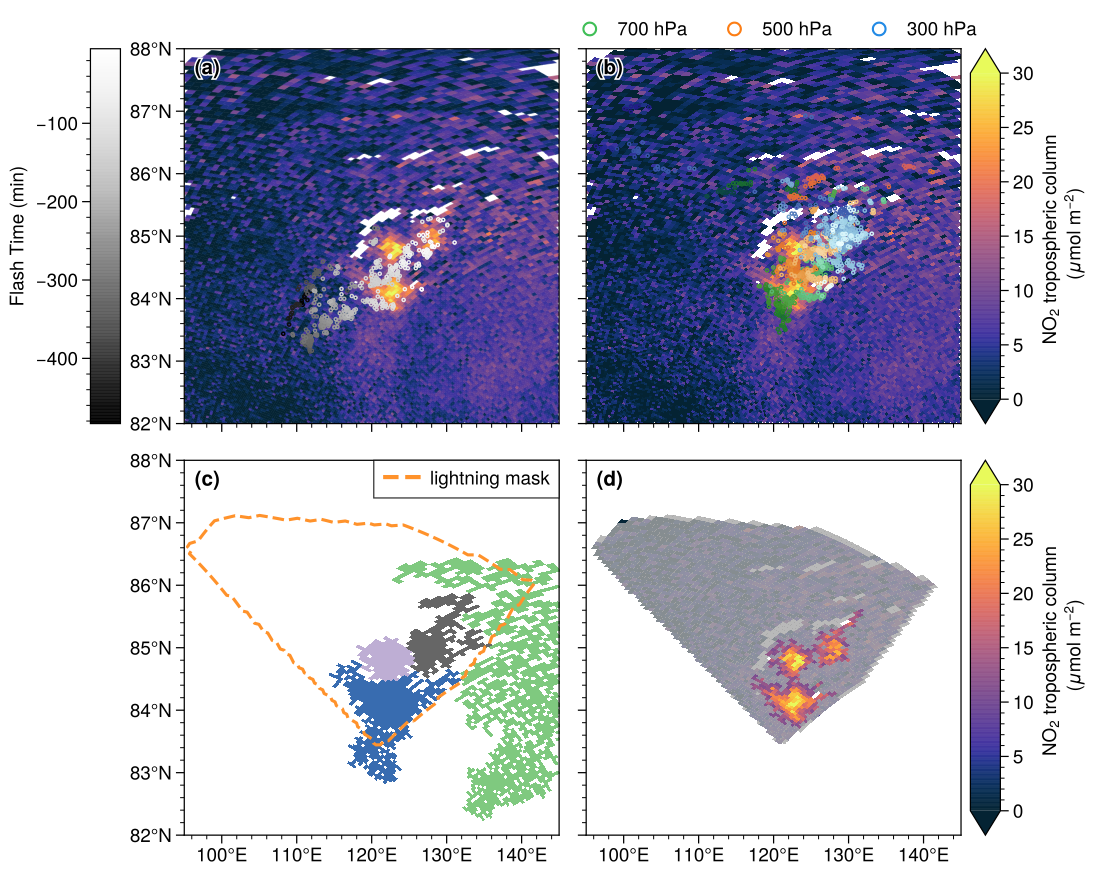
\includegraphics[width=0.9\textwidth]{./figures/arctic_workflow.png}
\caption{
从 TROPOMI 轨道 09458(2019 年 8 月 1 日)数据筛选闪电 NO$_{\ch{2}}$ 像素的示意图,
背景填色为TROPOMI 检测到的 NO$_{\ch{2}}$ 对流层柱浓度。
(a)观测到的闪击;
(b)在三个气压层(300 hPa、500 hPa 和 700 hPa)上水平传输的闪电 NO$_{\ch{2}}$ 空气块;
(c)将空气块组合成一个闪电掩膜(橙色框),与高 NO$_{\ch{2}}$高值区(填充像素)相重叠。
不同的像素颜色代表基于多个 NO$_{\ch{2}}$ 阈值的不同 NO$_{\ch{2}}$ 选区;
(d)掩膜内受闪电 NO$_{\ch{2}}$ 影响的 NO$_{\ch{2}}$ 对流层柱浓度最终选区(亮色像素)。\\
Figure \ref{fig:workflow}. Overview of the process for identifying lightning NO$_{\ch{2}}$ pixels from TROPOMI orbit 09458 on August 1, 2019.
The TROPOMI-detected NO$_{\ch{2}}$ tropospheric columns are overlaid with (a) observed lightning strokes and
(b) transported air parcels of lightning NO$_{\ch{2}}$ at three pressure levels [300 hPa (blue), 500 hPa (orange), and 700 hPa (green)].
(c) Parcels are combined into one lightning mask (orange circle), which overlaps with high NO$_{\ch{2}}$ selections (filled pixels). The different pixel colors represent different NO$_{\ch{2}}$ selections based on multiple NO$_{\ch{2}}$ thresholds.
(d) Final selection (bright colored pixels) of NO$_{\ch{2}}$ tropospheric columns affected by lightning NO$_{\ch{2}}$ within the mask.
}
\label{fig:workflow}
\end{figure}


\subsection*{计算闪电二氧化氮柱浓度}

\citet{Zhang.2022a}指出官方 TROPOMI 算法在 NO$_{\ch{2}}$反演中不包括 LNO$_{\ch{2}}$,
因此本研究从官方 $S_{\ch{NO2}}$产品中减去背景 NO$_{\ch{2}}$,并将差值通过大气质量因子(AMF)转换为对流层LNO$_{\ch{2}}$垂直柱浓度。
该算法具体为下式
\begin{equation} \label{eq:arctic_LNO2}
V_{\ch{LNO_2}} = \frac{S_{\ch{NO_2}} - S_{\ch{BG}}}{AMF_{\ch{LNO_2Clean}}}
\end{equation}
其中 $V_{\ch{LNO2}}$ 是对流层 LNO$_{\ch{2}}$ 垂直柱浓度,
$S_{\ch{NO2}}$ 是 TROPOMI 测得的对流层 NO$_{\ch{2}}$ 斜柱浓度,
$AMF_{\ch{LNO2Clean}}$ 是LNO$_{\ch{2}}$大气质量因子。
根据\citet{Allen.2021a},本研究将背景 $S_{\ch{NO2}}$($S_{\ch{BG}}$)定义为对流层 AMF 和在闪电掩膜内NO$_{\ch{2}}$低值区的第 30 个百分位数$V_{\ch{NO2}}$的乘积。
NO$_{\ch{2}}$低值区(图 \ref{fig:workflow}d中的灰色像素)是由分水岭方法得到的$V_{\ch{NO2}}$高值区之外的所有掩膜像素。
$AMF_{\ch{LNO2Clean}}$ 是“可见”LNO$_{\ch{2}}$ 斜柱浓度与对流层 LNO$_{\ch{2}}$ 垂直柱浓度之比,即式(\ref{eq:AMF_LNO2clean}),
其中$LNO_2(p)$ 是与气压有关的先验 LNO$_{\ch{2}}$高斯分布廓线,

由于北极地区排放源及对流模拟结果不确定性较大,本文利用基于云压假设的高斯分布来作为LNO$_{\ch{2}}$廓线,
高斯分布的峰值高度为最高(数值最小)的$p_{cloud}$,峰宽设置为180 hPa。
该峰值宽度是由高斯分布拟合前人的LNO$_{\ch{x}}$廓线得到的,具体由方程 $k*e^\frac{{-{(p - peak\_pressure)}^2}}{2*peak\_width^{2}}$ 给出,
其中$p$ 是TM5的气压层,系数 $k$ 在 AMF 计算中同为分子和分母所以被抵消。
利用该公式拟合 \citet{Ott.2010} 的海洋型LNO$_{\ch{x}}$廓线和\citet{Luo.2017}的中纬度大陆型LNO$_{\ch{x}}$廓线,
得到$peak\_width$ 的平均值为180 hPa(图\ref{fig:arctic_lnox_profile})。
本研究没有使用\citet{Ott.2010}中的中纬度大陆 LNO$_{\ch{x}}$ 廓线,是由于\citet{Luo.2017}指出该廓线与对流前的廓线相似,而本研究需要对流时的廓线。
与 $peak\_width$ 和云压相关的 LNO$_{\ch{2}}$ 产率不确定性见表\ref{table:arctic_uncertainty}。
此外北极地区对流云的$p_{cloud}$范围为130--987 hPa,主要集中于250--300 hPa最常见的值(图\ref{fig:pcld_ptropo})。
由于云内部的NO$_{\ch{2}}$浓度高,而云层之上的NO$_{\ch{2}}$由于光解作用而浓度低,故假设的LNO$_{\ch{2}}$廓线较TM5模拟的NO$_{\ch{2}}$廓线更加真实\citep{Beirle.2009}。
对于高而厚的云层,云层上方的散射权重相当均匀,LNO$_{\ch{2}}$的灵敏度在云层中部附近最高,所以受LNO$_{\ch{2}}$廓线假设的影响已降到最低\citep{Laughner.2017}。
具体而言,$AMF_{\ch{LNO2}}$计算中使用的散射权重由五个参数决定:地表气压、太阳天顶角、视角天顶角、相对方位角和反照率。
对于多云部分,查找表中使用的地表气压和反照率采用云压和云反照率。
此外,本研究剔除了云层高于对流层顶的个例,因为 NO$_{\ch{2}}$ 浓度可能会受到平流层 O$_{\ch{3}}$ 的影响\citep{Frey.2015a,Zhang.2022a}。

\begin{figure}[H]
\centering
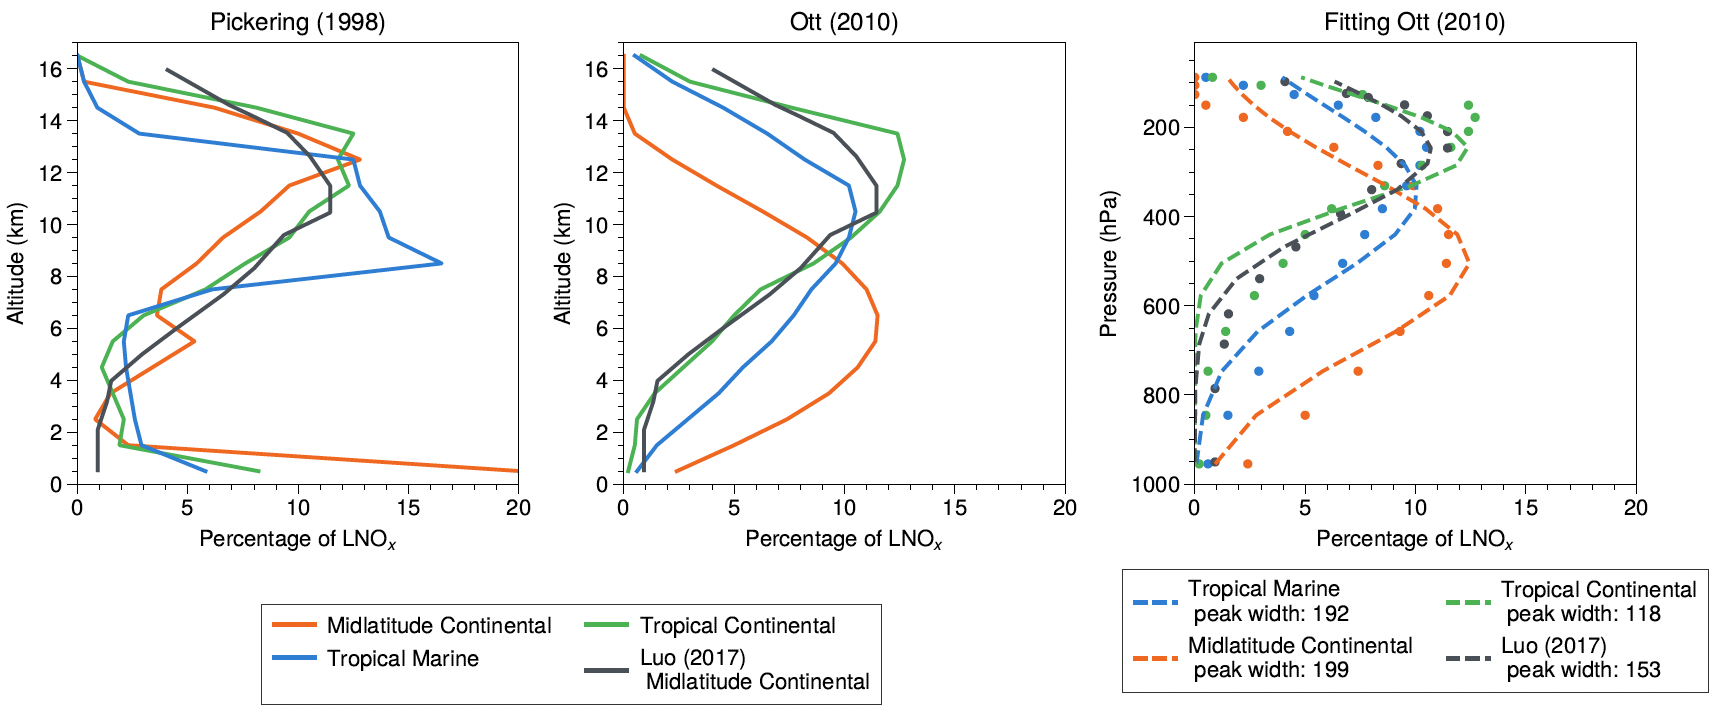
\includegraphics[width=\textwidth]{./figures/arctic_lnox_profile.png}
\caption{
每公里LNO$_{\ch{x}}$质量百分比的平均垂直分布。
数据来源:(a)\  \citet{Pickering.1998};(b)\  \citet{Ott.2010},
来自\  \citet{Luo.2017} 的 LNO$_{\ch{x}}$ 廓线以黑色显示;
(c) 高斯拟合曲线(虚线)和原始数据(散点)。\\
Figure \ref{fig:arctic_lnox_profile}.
Average vertical distributions of percentage of typical LNO$_{\ch{x}}$ mass per kilometer.
The LNO$_{\ch{x}}$ profiles are from (a)\ \ \citet{Pickering.1998} and (b)\ \ \citet{Ott.2010}.
The LNO$_{\ch{x}}$ profile from\ \ \citet{Luo.2017} is shown in black.
(c)  The Gaussian fitting profiles (dashed lines) and the original data (scatter points).
}
\label{fig:arctic_lnox_profile}
\end{figure}

\begin{figure}[H]
\centering
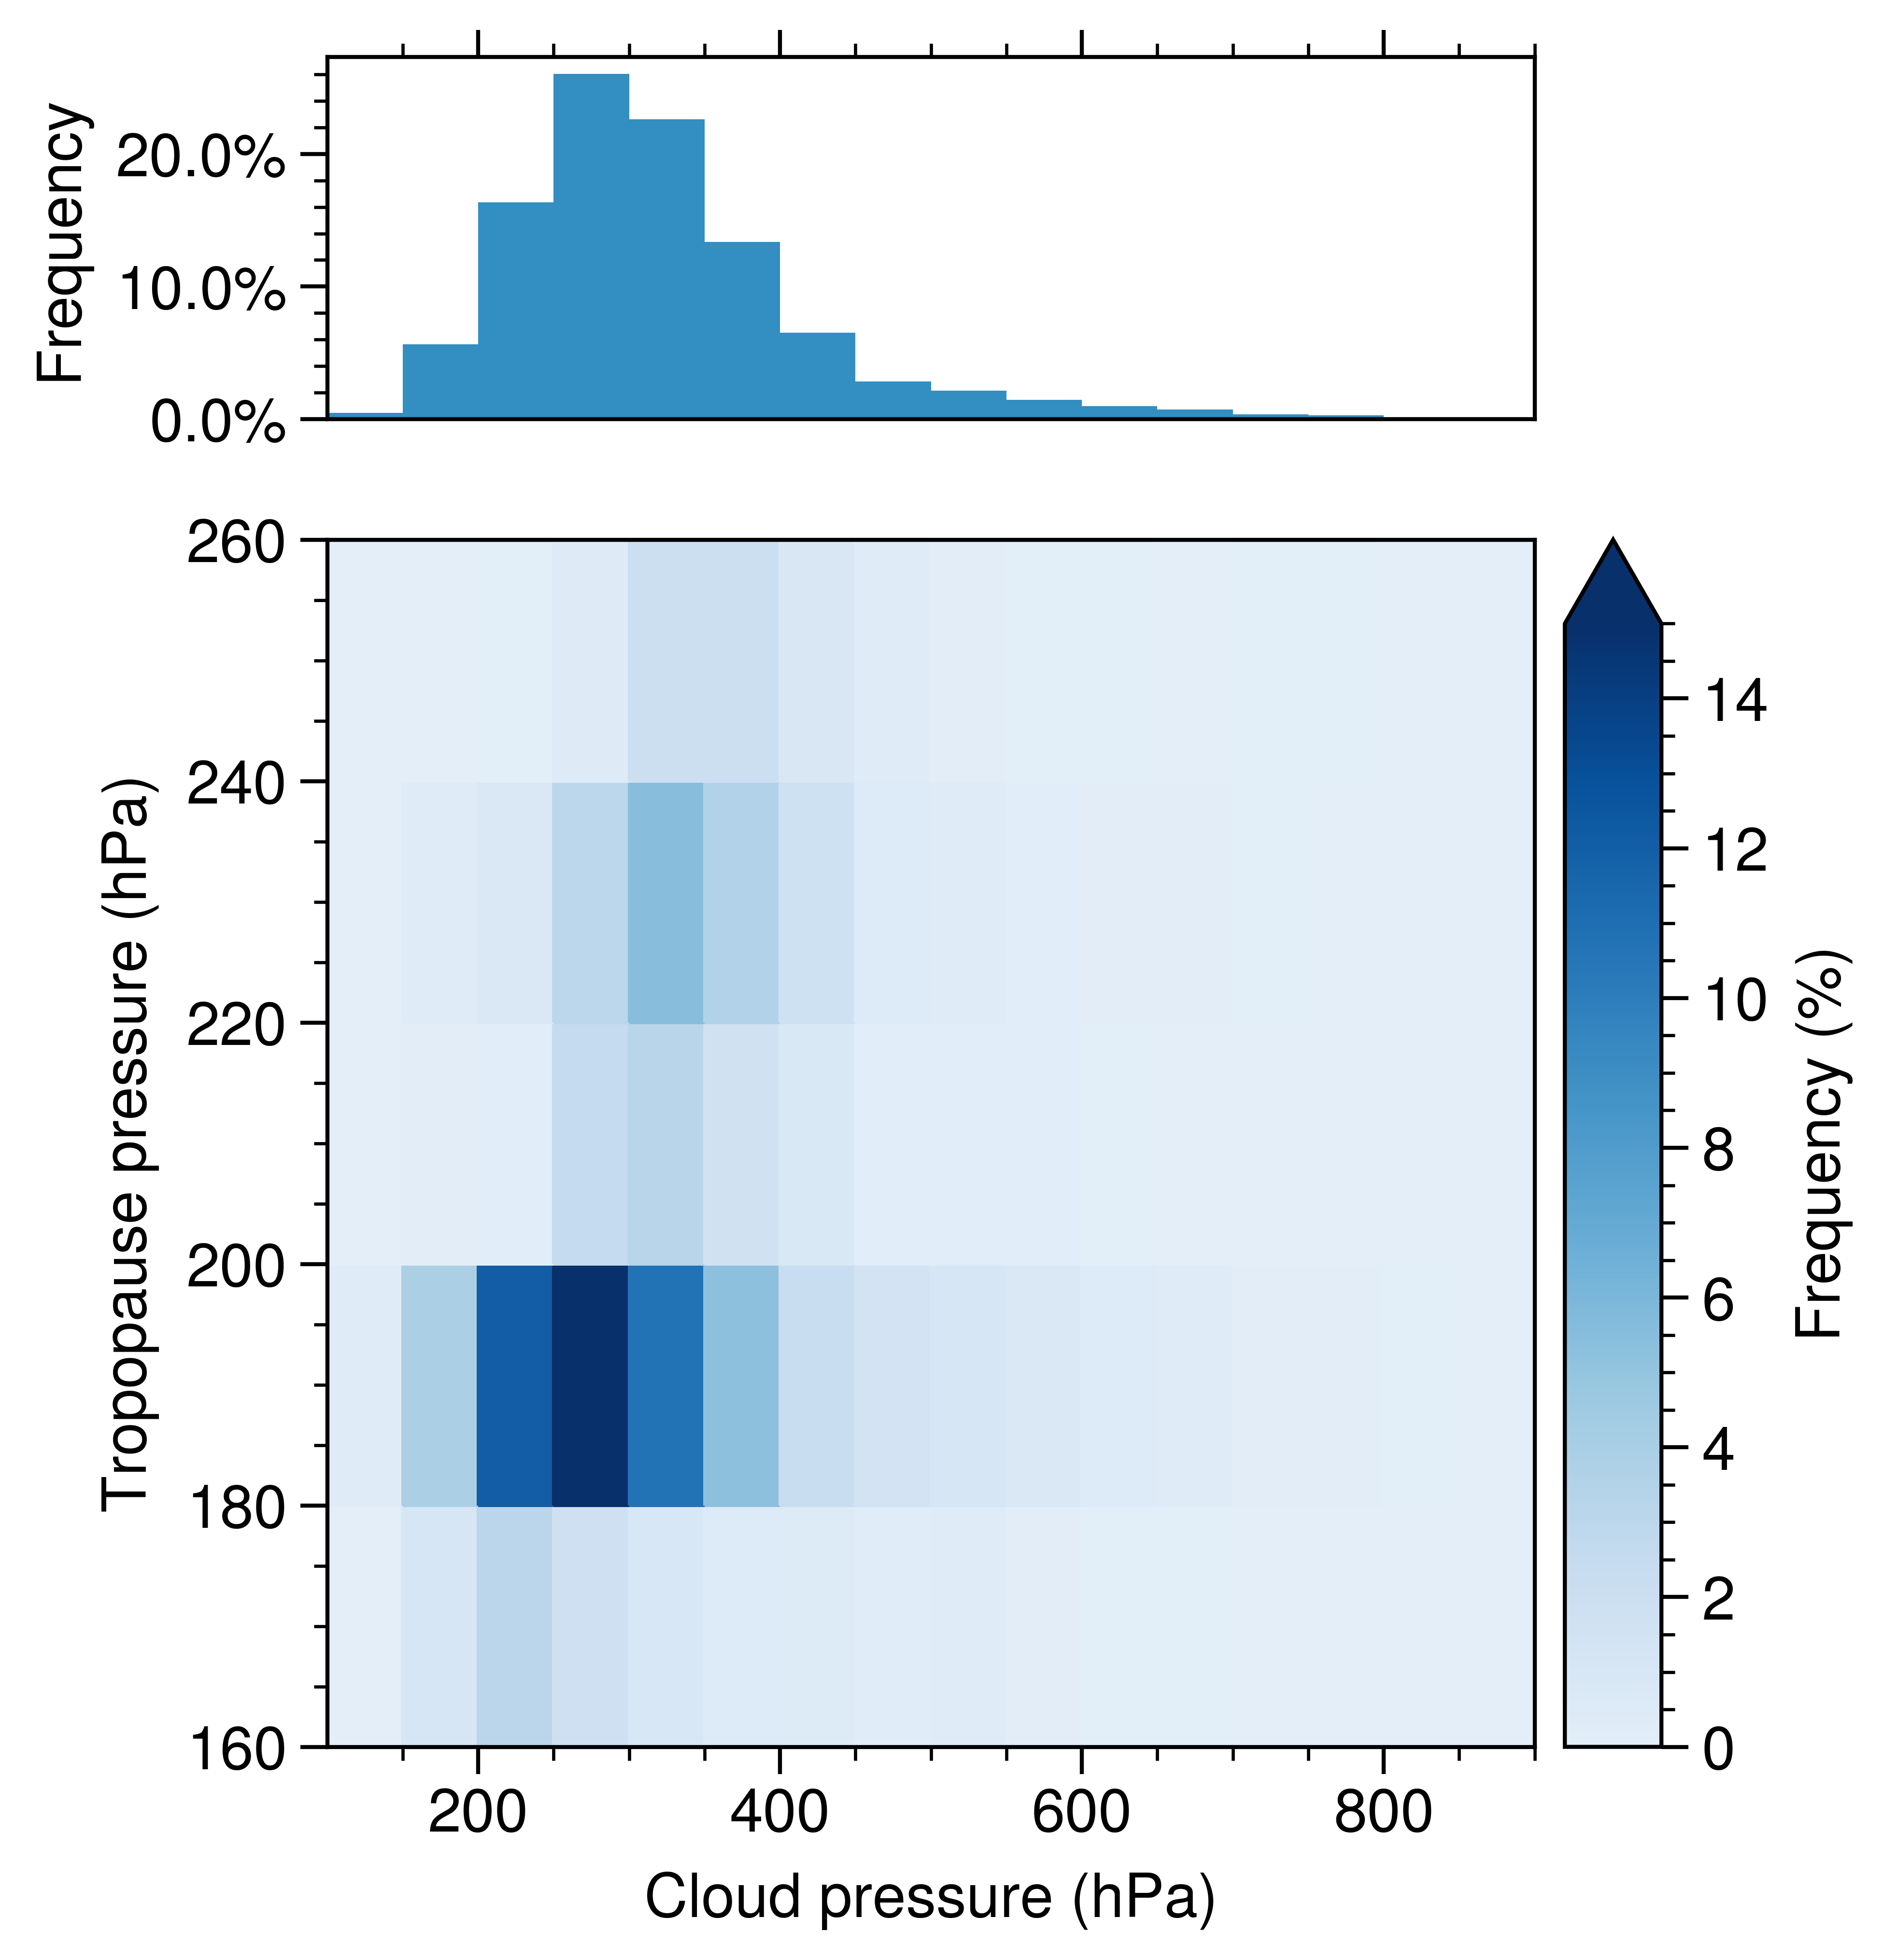
\includegraphics[width=0.6\textwidth]{./figures/pcld_ptropo.png}
\caption{云辐射分数大于0.7的像素上TROPOMI测得的云压和对流层顶高度直方图。\\
Figure \ref{fig:pcld_ptropo}. The histogram of TROPOMI cloud pressure and tropopause pressure over lightning
pixels with the cloud radiance fraction larger than 0.7.
}
\label{fig:pcld_ptropo}
\end{figure}


\begin{table}[H]
\centering
\caption{LNO$_{\ch{2}}$产率估算的不确定性$^a$\\
Table \ref{table:arctic_uncertainty}. Uncertainties$^a$ for the estimation of LNO$_{\ch{2}}$ production efficiency (PE).}
\label{table:arctic_uncertainty}
\footnotesize
{\centering
\begin{tabular}{llll}
\thickline
类型                           &  默认值        & 扰动                 &   不确定度 (\%)  \\
\thickline
LNO$_{\ch{2}}$ 寿命                   & 3 小时                 & 2 小时和4 小时$^b$      &   36                      \\
IC:CG                         & 1:1                    & 2:1和1:2                  &   33 \\
LNO$_{\ch{2}}$ 廓线宽度                & 180 hPa               & 160 hPa 和 200 hPa          &   7   \\
NO$_{\ch{2}}$ 对流层背景浓度      & 第 30 个百分位数        & 第 10 个百分位数$^c$     & 2                \\
LNO$_{\ch{2}}$ 选区              & 80\% 置信区间          &  70\% 置信区间   & 13                \\
云压                 & 二级产品               &  $\pm$ 50 hPa$^d$                & 7                \\
其他$^e$       & --                  & --                           &   10                      \\
净不确定度                            &                     &                              &   53                      \\
\thickline
\end{tabular}
\par }
\begin{tablenotes}
\linespread{1}\footnotesize
\item $^a$ 不确定度 = (误差$_{\ch{高扰动值}}$ - 误差$_{\ch{低扰动值}}$)/2,
其中 误差$_{\ch{扰动}}$ = (PE$_{\ch{扰动}}$ - PE$_{\ch{默认值}}$)/PE$_{\ch{默认值}}$;
\item $^b$ 基于本研究得到的寿命范围。
\item $^a$ Uncertainty = (Error$_{rising\ perturbed\ value}$ - Error$_{lowering\ perturbed\ value}$)/2
where Error$_{\* perturbed\ value}$ = (PE$_{\* perturbed\ value}$ - PE$_{default\ value}$)/PE$_{default\ value}$.
\item $^b$ Based on the lifetime values calculated in this study.
\item $^c$ \ \citet{Allen.2021a} and \ \citet{Perez-Invernon.2022}.
\item $^d$ \ \citet{VanGeffen.2022}.
\item $^e$ \ \citet{Allen.2021a}.
\end{tablenotes}
\end{table}


\subsection*{计算闪电二氧化氮产率} \label{sec:calc_lnox_pe}

如\ref{subsect:lightning_distribution}节所述,TROPOMI 可多次扫过 70$^{\circ}$ N 以北的同一点,
因此两个连续的轨道可以观测到相同的雷暴系统。
为了更方便地分析北极 LNO$_{\ch{2}}$ 个例,本研究开发了可视化网站(\url{https://arctic-lightning-no2.streamlit.app/}),
允许用户筛选个例并交互式研究LNO$_{\ch{2}}$、云压和闪电之间的关系。
$V_{\ch{LNO2}}$(mol m$^{-2}$)在相邻过境时间之间的关系可以定义为:
\begin{equation} \label{eq:relationship}
\sum_{p_{(T2)}} V_{\ch{LNO_2_i}} A_{i} = e^\frac{{-(T_2-T_1)}}{\tau} \sum_{p_{(T1)}} V_{\ch{LNO_2_j}} A_{j} + PE \sum_{N} e^\frac{{-(T_2-t_k)}}{\tau}
\end{equation}
其中 $p$ 是 LNO$_{\ch{2}}$ 区域中的像素数,
$A$ 是每个像素的面积(m$^2$),
$T$ 是 TROPOMI 过境时间,
$t$ 是闪电发生的时间,
$\tau$ 是对流附近 LNO$_{\ch{2}}$ 的寿命,
$PE$ 是 LNO$_{\ch{2}}$ 的产率(mol NO$_{\ch{2}}$ 每闪击),
$N$ 是在相邻过境时间内发生的总闪击数,
而指数成分考虑了 NO$_{\ch{2}}$ 的化学损失。
除此之外,$i$ 和 $j$ 是 TROPOMI 的像素索引,
$A_{i}$ 和 $A_{j}$ 是不同的 LNO$_{\ch{2}}$ 区域,并考虑了平流的影响(图\ref{fig:consecutive_orbits}),
$T_1$ 和 $T_2$ 代表 TROPOMI 在 LNO$_{\ch{2}}$ 区域的两次平均过境时间,
$t_k$ 代表两个轨道之间发生的第 k 次闪击(k 取值范围为 1 到 N)的时间。

如果相邻过境时间内没有闪电发生,式(\ref{eq:relationship})可以简化为:

\begin{equation} \label{eq:LNO2_nolightning}
\sum_{p_{(T2)}} V_{\ch{LNO_2}_i} A_{i} = e^\frac{{-(T_2-T_1)}}{\tau} \sum_{p_{(T1)}} V_{\ch{LNO_2}_j} A_{j}
\end{equation}
本研究通过分析具有高 LNO$_{\ch{2}}$ 但两次过境时间之间没有闪电的特殊个例,得到 $\tau$ 值为 3 $\pm$ 1 h(表\ref{table:lifetime} 和图 \ref{fig:consecutive_orbits}),
并将其代入式(\ref{eq:relationship})来计算剩余个例的LNO$_{\ch{2}}$产率。


在前人的研究中共有三种方法来估算热带和中纬度地区的 LNO$_{\ch{2}}$ 产量:

(1) 背景NO$_{\ch{2}}$与LNO$_{\ch{2}}$之和(LNO$_{\ch{2}}$$^*$)与闪电之间的线性回归 \citep{Pickering.2016,Allen.2019,Lapierre.2020};

(2) 使用自定义的大气质量因子直接得到LNO$_{\ch{2}}$ \citep{Beirle.2009,Zhang.2020b,Zhang.2022a};

(3) 从LNO$_{\ch{2}}$$^*$中减去背景 NO$_{\ch{2}}$,其中背景 NO$_{\ch{2}}$取自飞机观测 \citep{Pickering.2016,Perez-Invernon.2022} 或未发生闪电的对流像素处的平均NO$_{\ch{2}}$柱浓度 \citep{Bucsela.2019,Bucsela.2010,Allen.2021a}。

由于背景 NO$_{\ch{2}}$ 随太阳天顶角而变化,线性回归法不适用于北极地区。
第二种方法需要使用闪电参数化进行详细的 LNO$_{\ch{2}}$ 模拟,而目前闪电参数化的不确定性仍非常大\citep{Finney.2018,Romps.2019,Chen.2021a},尤其是在闪电数据集很少的北极地区 \citep{Holzworth.2021}。
因为 TROPOMI 检测到70$^{\circ}$ N 以北的非闪电对流个例有限,
所以最后一种方法需要的平均背景 NO$_{\ch{2}}$数据集也不适用于北极地区的网格(即 1 $^{\circ}$ $\times$ 1 $^{\circ}$)。

\begin{table}[H]
\centering
\caption{2019--2021期间得到的闪电 NO$_{\ch{2}}$(LNO$_{\ch{2}}$)寿命\\
Table \ref{table:lifetime}. Lightning NO$_{\ch{2}}$ (LNO$_{\ch{2}}$) lifetimes derived from cases (2019--2021).}
\label{table:lifetime}
\footnotesize
{\centering
\begin{tabular}{llllll}
\thickline
时间             &         轨道 &    经度 &   纬度 &  $\Delta$面积(\%)$^a$ &  寿命(h)\\
\thickline
2019-06-28 00:38 &       08833 &  127.4 &  81.0 &     -14.5 &       3.0 \\
2019-08-14 22:58 &       09513 &  126.0 &  70.4 &       2.0 &       1.7 \\
2020-06-09 19:11 &       13767 &  162.8 &  73.0 &     -43.8 &       3.6 \\
2020-06-15 22:18 &       13854 &  155.6 &  78.7 &      -4.4 &       3.4 \\
2020-07-15 21:19 &       14279 &  109.3 &  75.4 &       4.5 &       2.7 \\
2021-07-11 11:40 &       19395 &  -84.5 &  70.9 &      28.0 &       5.2 \\
\thickline
\end{tabular}
\par }
\begin{tablenotes}
\linespread{1}\footnotesize
\item $^a$$\Delta$面积 是 LNO$_{\ch{2}}$ 面积在 $T_2$ 时刻相对于 $T_1$ 时刻的百分比变化
($T_1$ 和 $T_2$ 是连续条带的平均过境时间,$T_2$ > $T_1$)。
\item $^a$$\Delta$Area is the percentage change of the LNO$_{\ch{2}}$ area at $T_2$ relative to $T_1$
($T_1$ and $T_2$ are the mean overpass time of consecutive swaths, $T_2$ > $T_1$).
\end{tablenotes}
\end{table}



\begin{figure}[H]
\centering
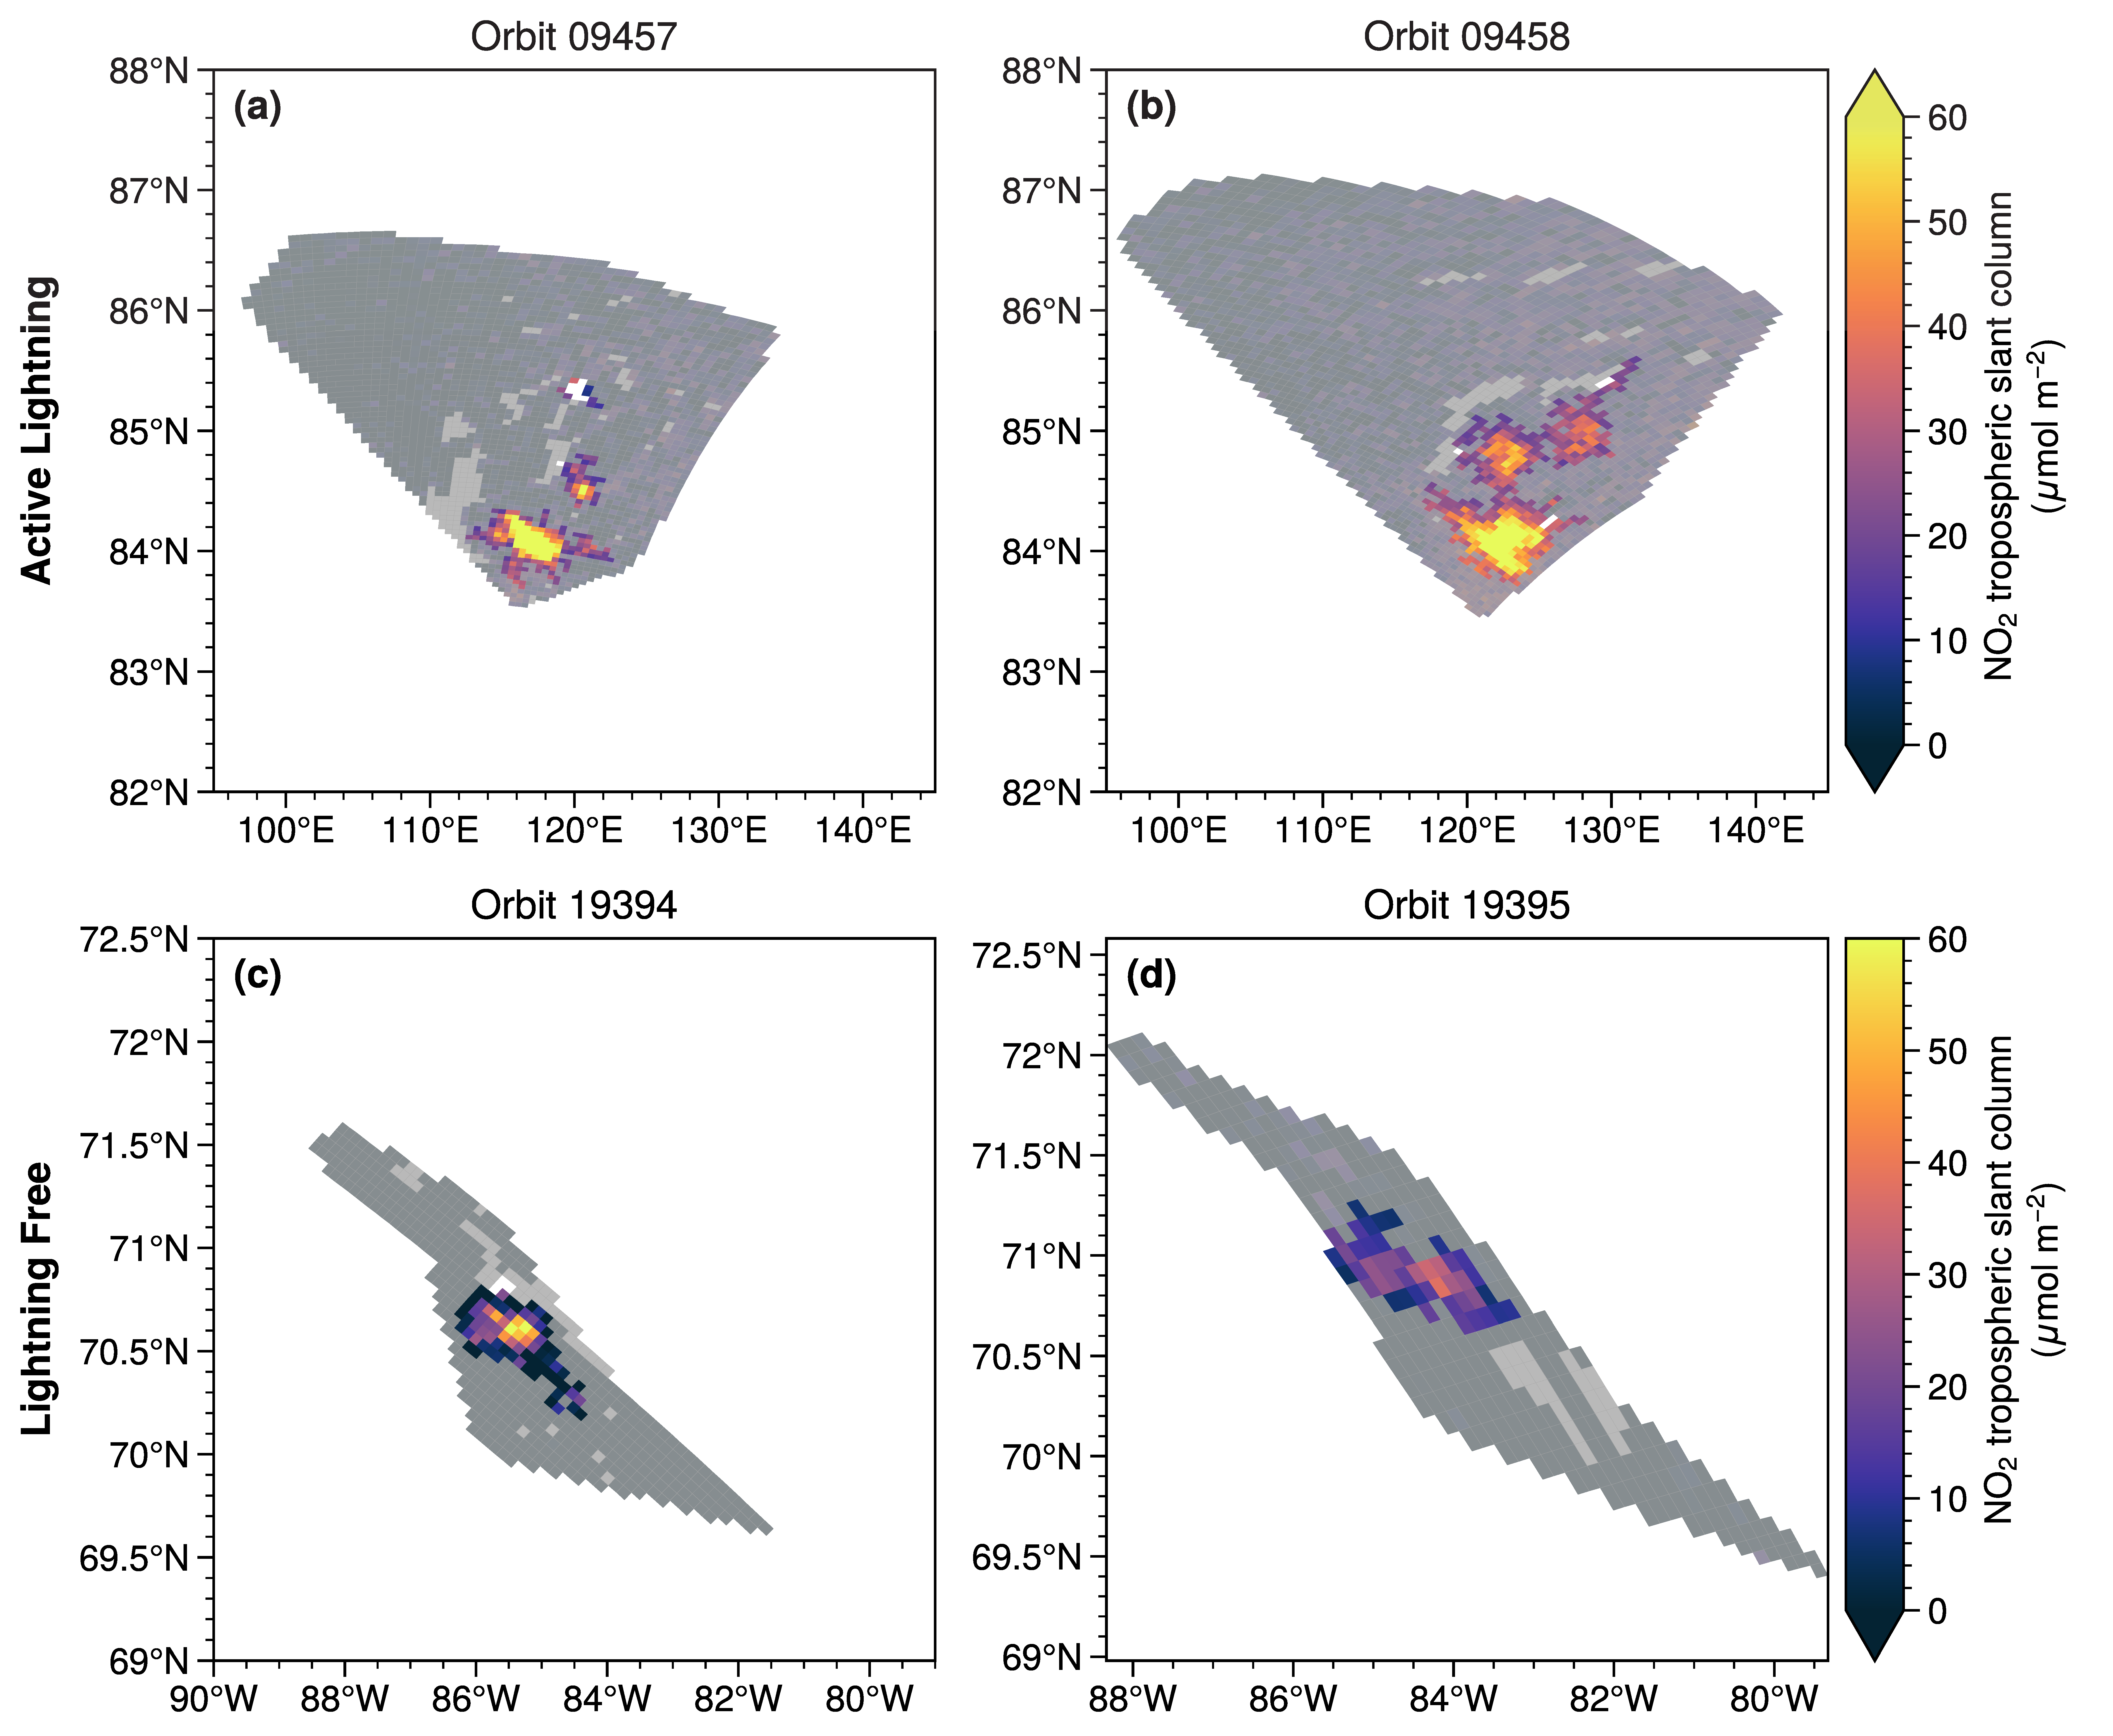
\includegraphics[width=0.85\textwidth]{./figures/arctic_consecutive_orbits.png}
\caption{
受闪电 NO$_{\ch{2}}$ 影响的 NO$_{\ch{2}}$ 对流层柱浓度选区(亮色像素)。
(a,b)两次连续的过境数据,且它们之间有活跃的闪电;
(c,d)两次连续的过境数据,但它们之间没有闪电。\\
Figure \ref{fig:consecutive_orbits}.
Selections (bright colored pixels) of NO$_{\ch{2}}$ tropospheric columns affected by lightning NO$_{\ch{2}}$.
(a--b) Two consecutive orbits with active lightning between them.
(c--d) Two consecutive orbits with no lightning between them.
}
\label{fig:consecutive_orbits}
\end{figure}


\subsection{闪电二氧化氮产率的海陆性差异}


LNO$_{\ch{2}}$ 排放是闪击数和 LNO$_{\ch{2}}$ 产率(每次闪击产生的LNO$_{\ch{2}}$)的乘积。
然而不可能根据来自单次过境的数据直接推导出 LNO$_{\ch{2}}$ 产率,
因为 TROPOMI 检测到的 LNO$_{\ch{2}}$ 由产生和消耗组成,所以时间维度上需要第二次过境数据。
本研究提出可以利用连续轨道的 LNO$_{\ch{2}}$ 来估算 LNO$_{\ch{2}}$ 产率(见\ref{sec:calc_lnox_pe}节)。
基于对 LNO$_{\ch{2}}$ 和闪击的筛选,本研究共获得了43个个例,115 个 LNO$_{\ch{2}}$ 选区。
其中60$^{\circ}$ W 和 180$^{\circ}$ W 之间的个例由于 LNO$_{\ch{2}}$ 不显著或没有足够的观测值而被剔除,
大多数个例位于 60$^{\circ}$ E 和 180$^{\circ}$ E 之间(图 \ref{fig:arctic_lno2_production}a)。
通过比较闪电分布(图 \ref{fig:arctic_lno2_production}a)与LNO$_{\ch{2}}$总和的分布(图 \ref{fig:arctic_lno2_production}b),
本研究发现 TROPOMI 观测到的 LNO$_{\ch{2}}$ 远离LNO$_{\ch{2}}$的排放源。
例如,喀拉海(Kara Sea)上没有闪电发生 (77--80$^{\circ}$ N, 65--105$^{\circ}$ E),
但此处的LNO$_{\ch{2}}$ 总共约为 5.1 $\times$ 10$^6$ mol,
这是由于对流层上层主导的东风对LNO$_{\ch{2}}$的输送作用,从而揭示了匹配闪电和 NO$_{\ch{2}}$的重要性。


尽管如此,LNO$_{\ch{2}}$ 与闪击之间仍有一致的空间相关性,因此本研究针对每个个例计算其 LNO$_{\ch{2}}$ 产率。
研究结果表明,LNO$_{\ch{2}}$ 产率在陆地、沿岸和海洋处为 2.0(第 25 至第 75 个百分位数:1.3--3.1)mol每闪击、
3.5(第 25 至第 75 个百分位数:1.1--13.0)mol每闪击
和11.5(第 25 至第 75 个百分位数:1.3--29.9)mol每闪击(图 \ref{fig:arctic_pe_rate}a)。
除了这些中值外,本研究还得到了排名前10的LNO$_{\ch{2}}$产率,其范围为每次闪击产生27--612 mol NO$_{\ch{2}}$(表\ref{table:arctic_pe_lno2}),
这些高值都出现在海洋或沿海地区。
由于个例数量有限,研究无法确定海洋和陆地之间的 LNO$_{\ch{2}}$产率是否存在统计学上的显著差异。
但在热带和中纬度地区的研究也表明,由于海洋上的闪电能量更高\citep{Beirle.2014,Hutchins.2013},
海洋上的 LNO$_{\ch{2}}$产率是陆地上的两倍\citep{Marais.2018,Allen.2019,Bucsela.2019}。

最近的研究表明,LNO$_{\ch{2}}$产率与闪电尺寸有关,尺寸越大,产生的LNO$_{\ch{2}}$越多 \citep{Huntrieser.2008,Marais.2018},
此外更强的上升气流与更小的闪电和更高的闪电频率相关\citep{Bruning.2013,Bruning.2015,Mecikalski.2015}。
因此,本研究计算了闪击率,即单位时间单位LNO$_{\ch{2}}$面积内的闪击次数,
它的范围从 2.3$\times$10$^{-10} $m$^{-2}$ h$^{-1}$ 到 4.1$\times$10$^{-6} $m$^{-2 }$ h$^{-1}$,
陆地地区闪击率(6.2$\times$10$^{-7}$ m$^{-2}$ h$^{-1}$)比海洋地区高$\sim$ 11 倍(5.2$\times$10$^{-8}$ m$^{-2}$ h$^{-1}$)。
本研究发现闪击率和 LNO$_{\ch{2}}$产率之间存在近似的幂律关系(图\ref{fig:arctic_pe_rate}b)。
当闪击率下降2个数量级时,LNO$_{\ch{2}}$产率增加10倍,这与中纬度地区的研究结果一致\citep{Bucsela.2019,Zhang.2020b}。

\begin{figure}[H]
\centering
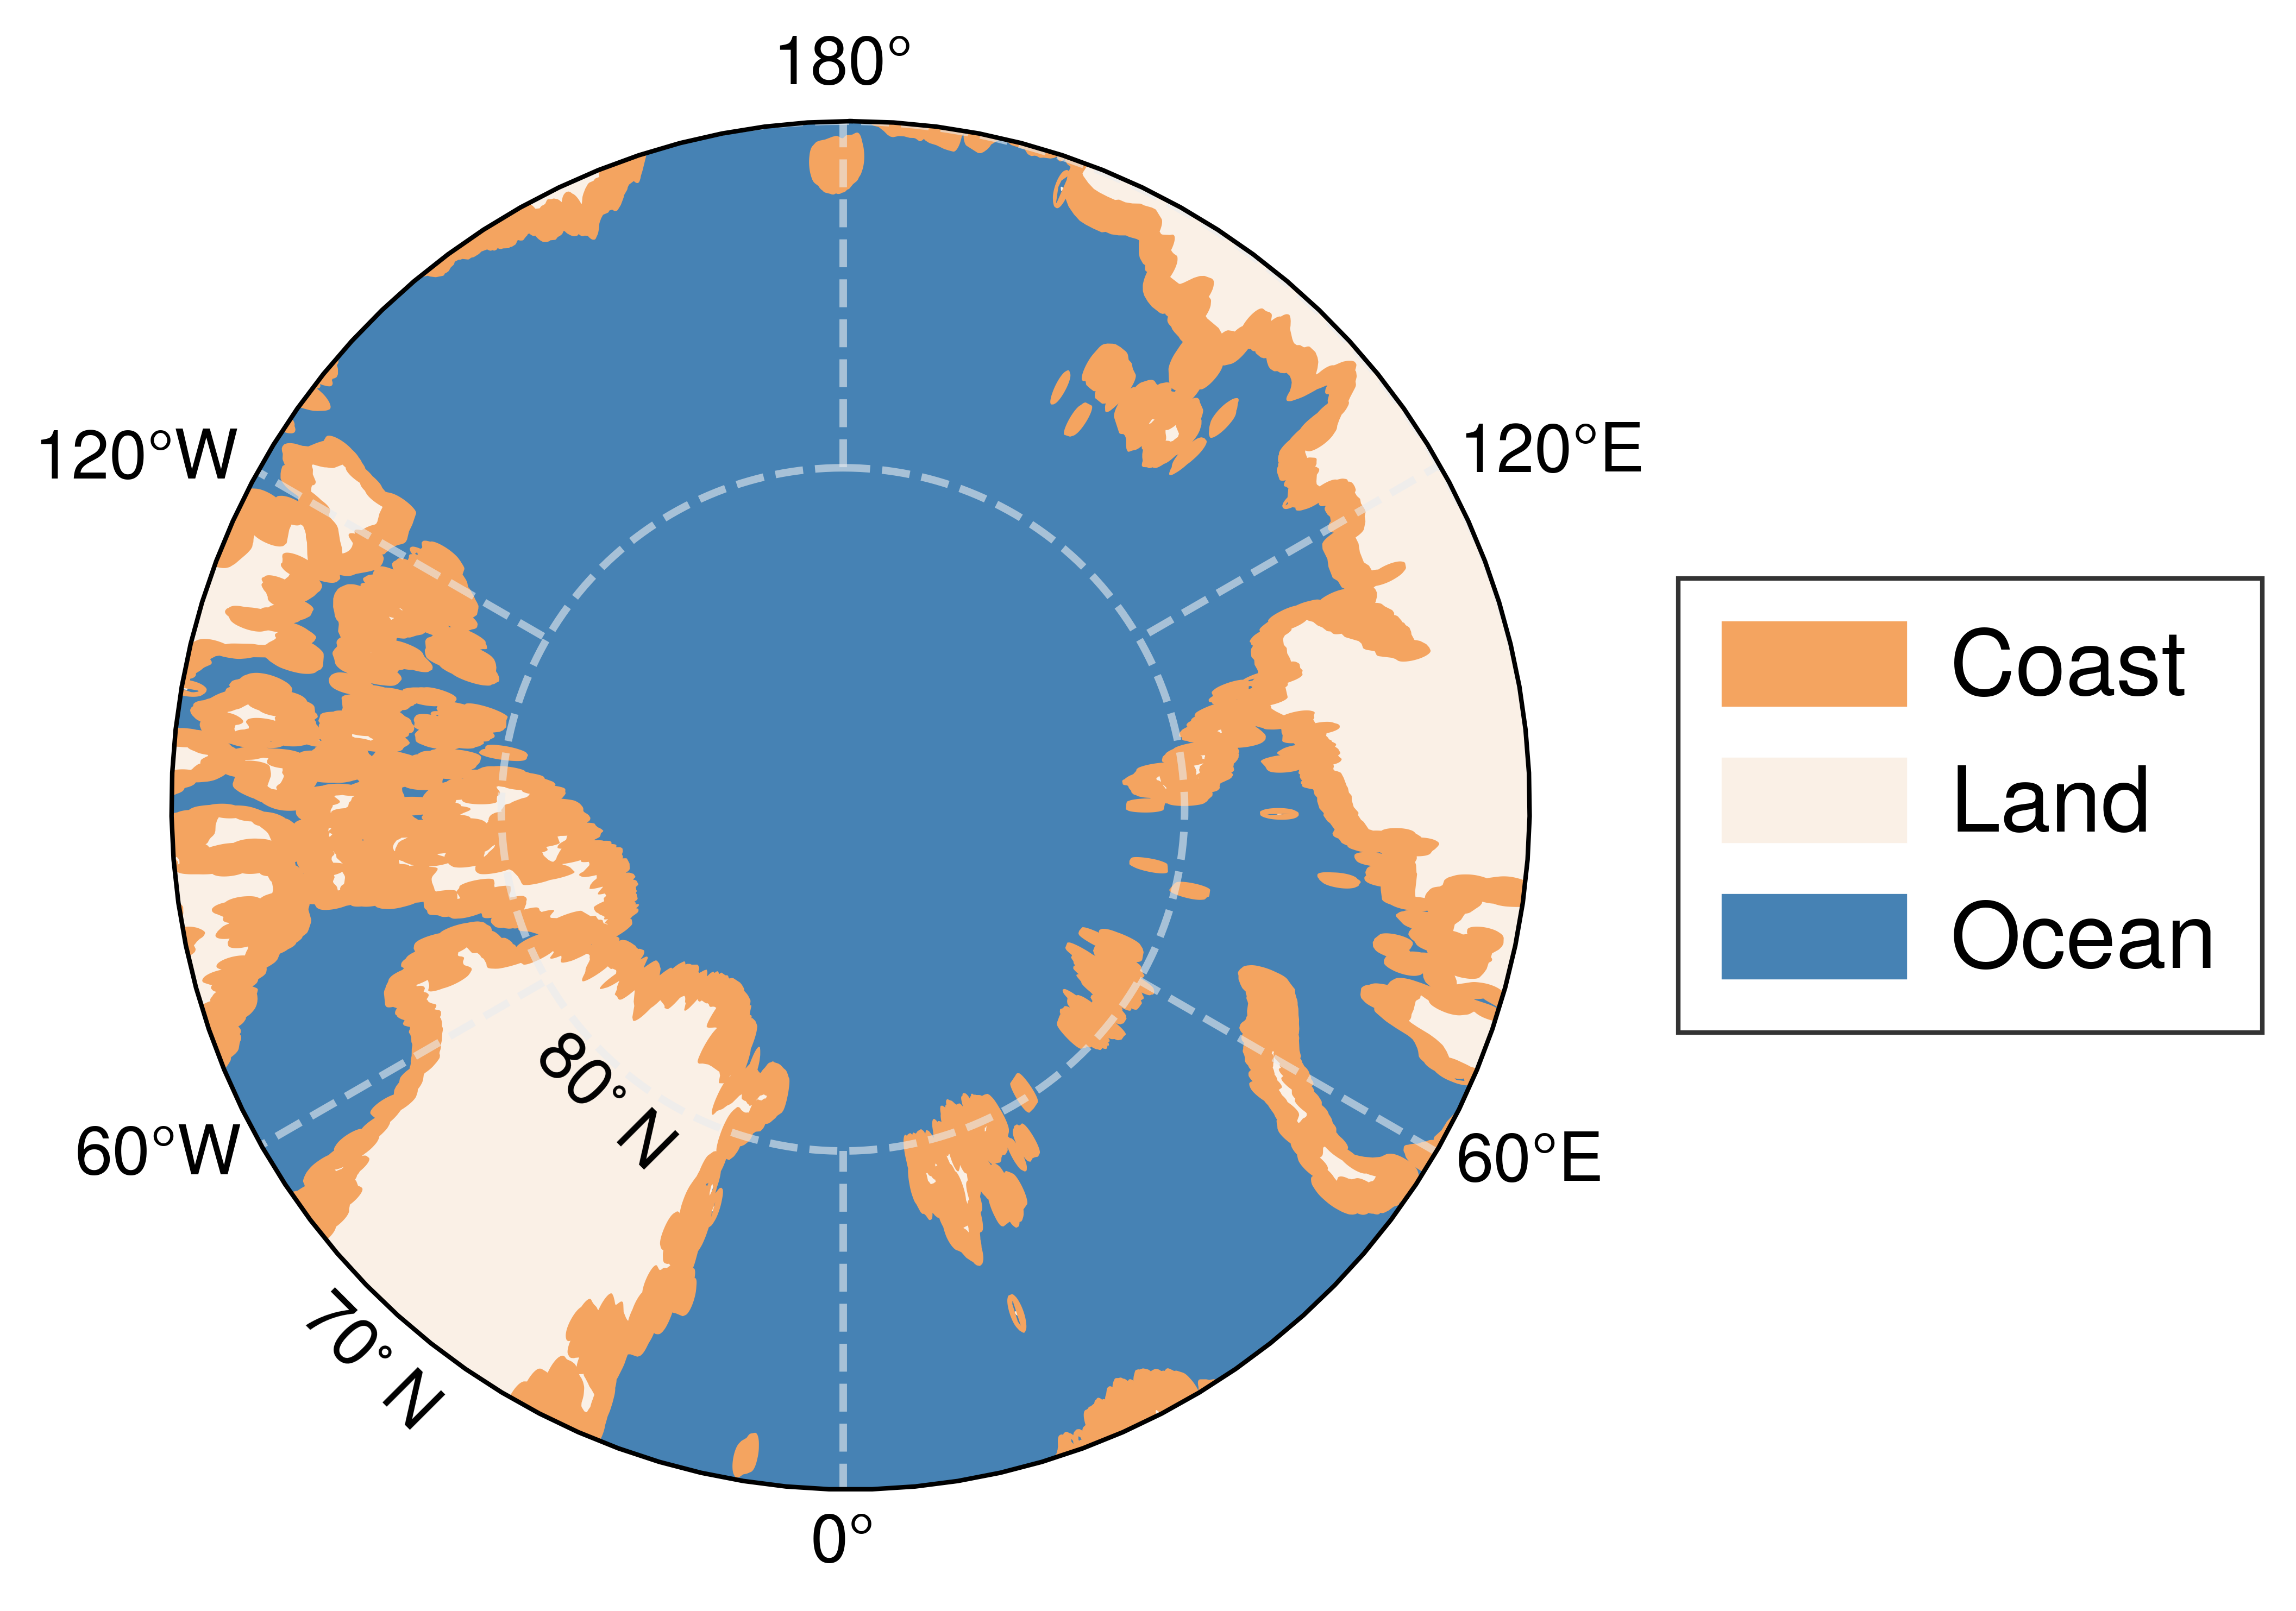
\includegraphics[width=0.65\textwidth]{./figures/arctic_region_mask.png}
\caption{
蓝色背景代表海洋,白色和橙色分别代表陆地和海岸,定义来自50 m自然地球数据。 \\
Figure \ref{fig:arctic_region_mask}. The blue background stands for the ocean, while the white and orange ones represent land
and coast, respectively. Definitions are from 50 m Natural Earth data.
}
\label{fig:arctic_region_mask}
\end{figure}


\begin{figure}[H]
\centering
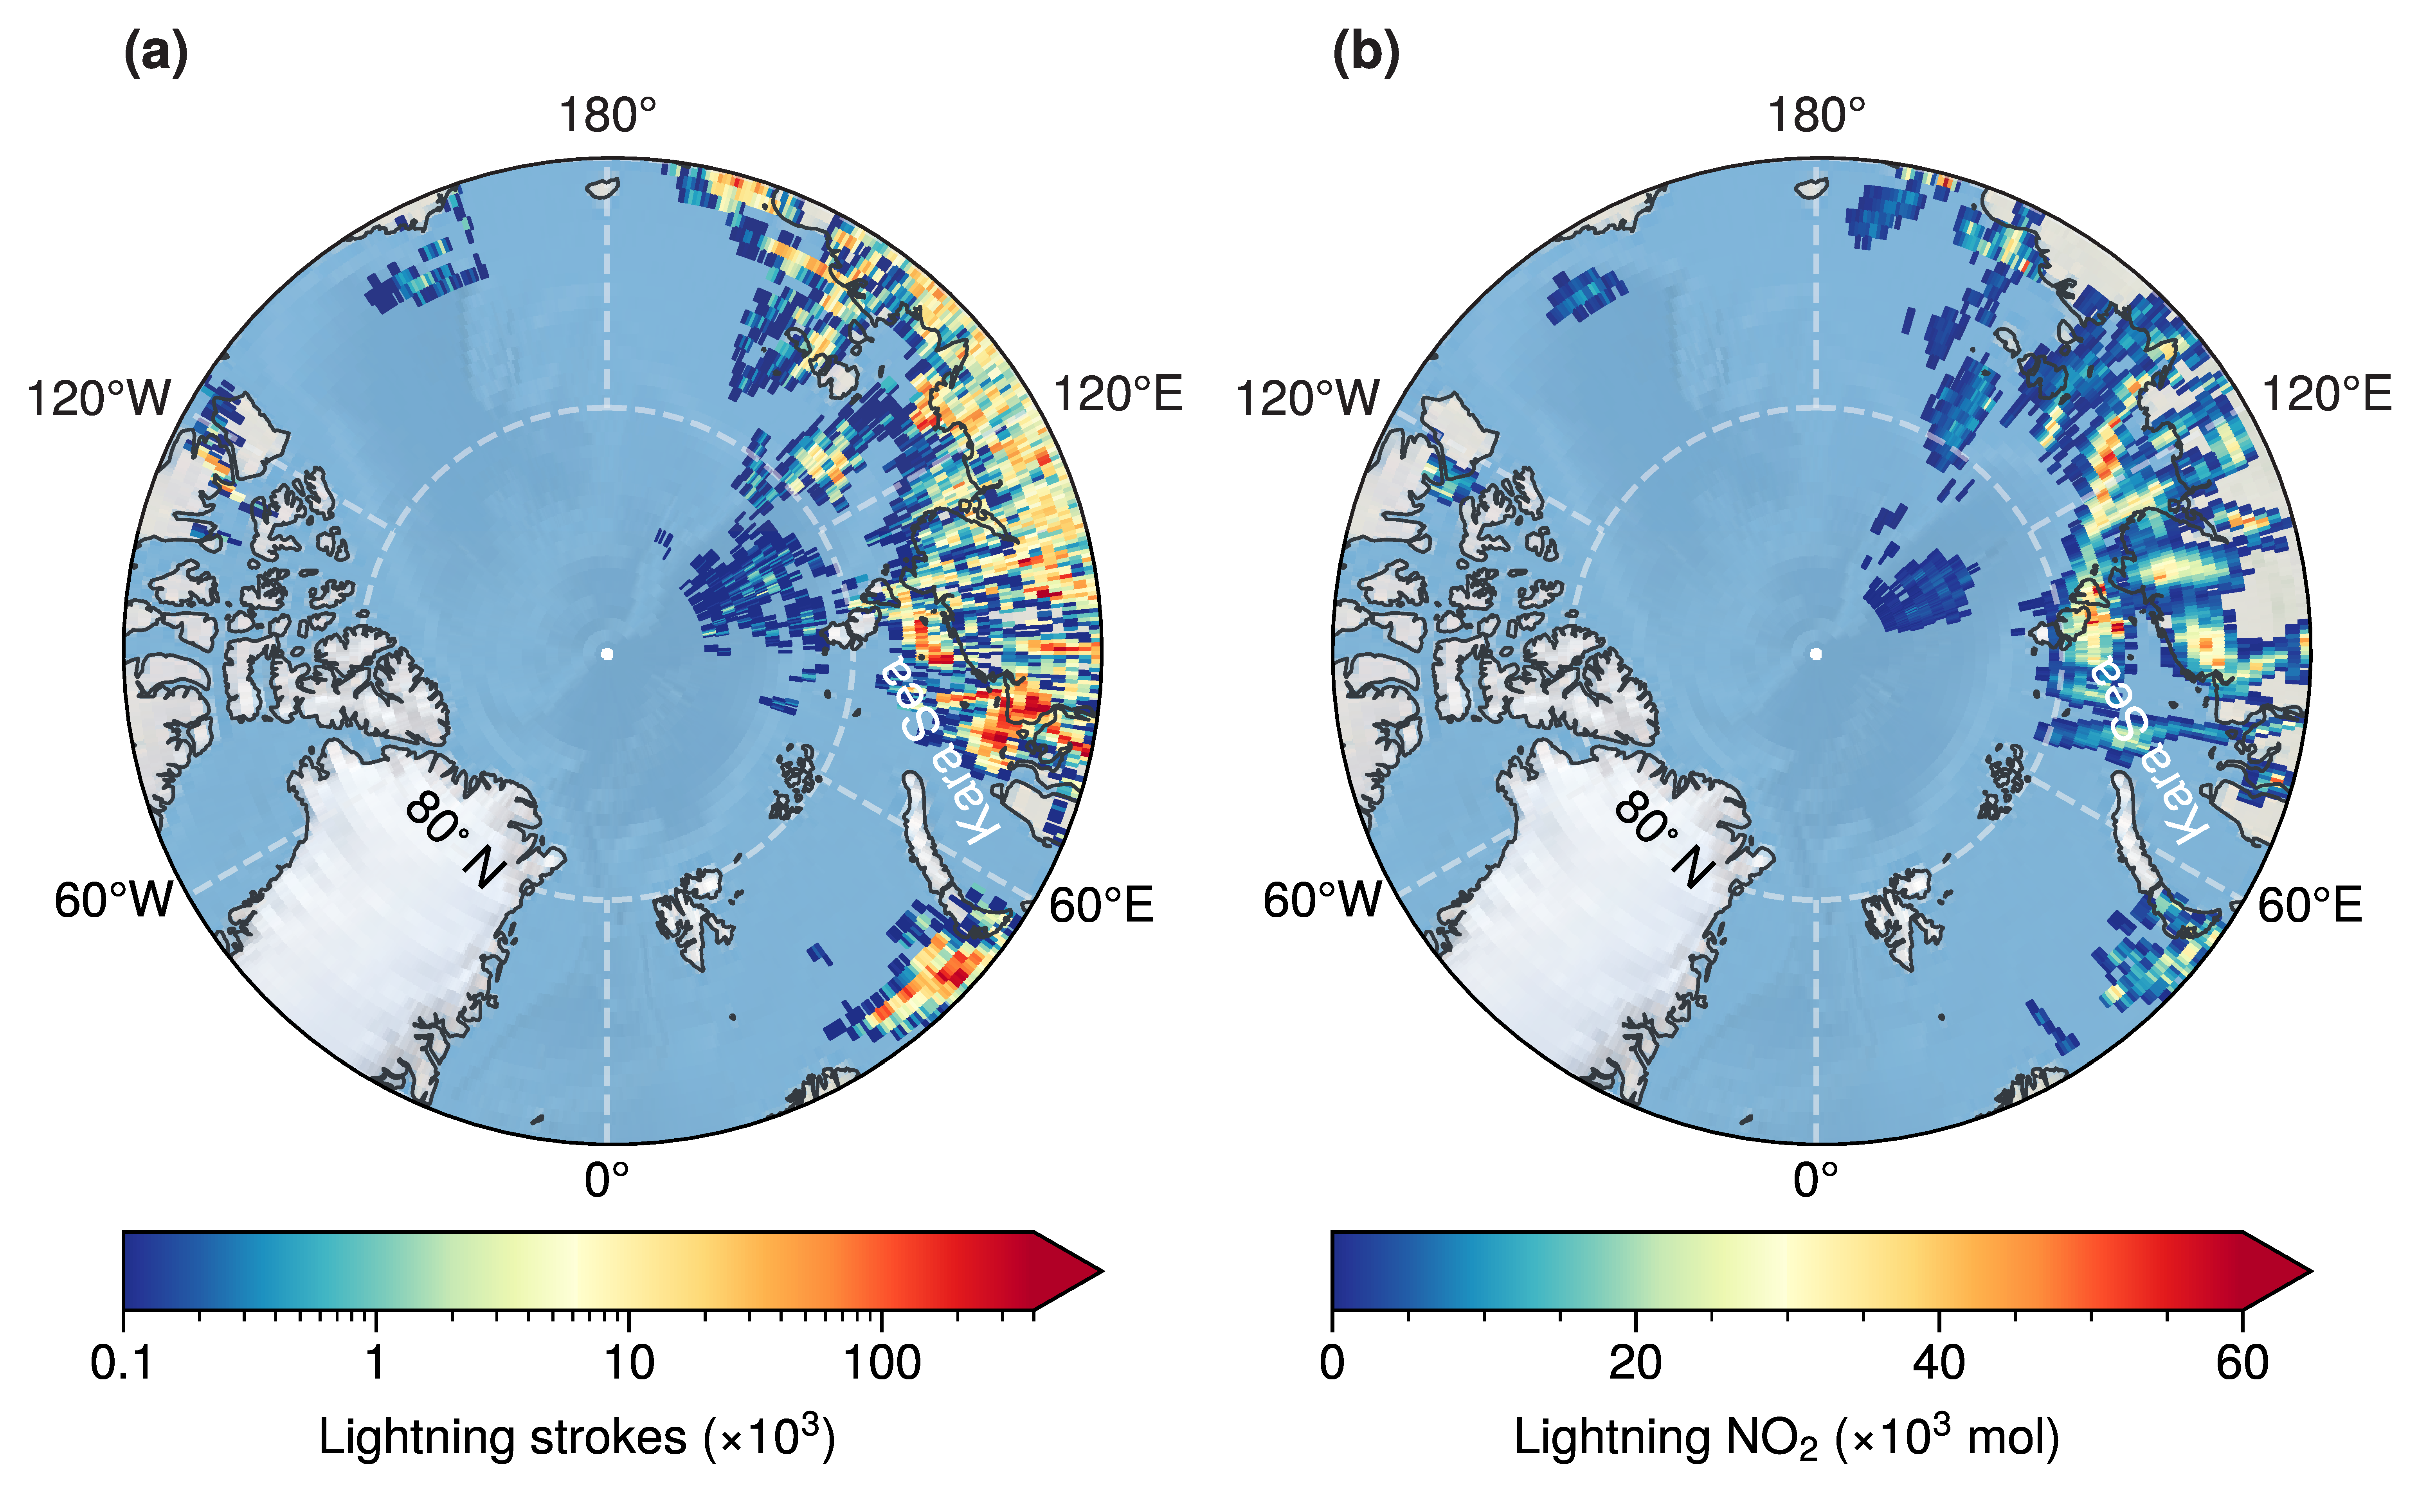
\includegraphics[width=0.9\textwidth]{./figures/arctic_lno2_production.png}
\caption{
(a)每 0.5$^{\circ}$ $\times$ 0.5$^{\circ}$ 网格中所选个例的 GLD360 闪击总和;
(b)每 0.5$^{\circ}$ $\times$ 0.5$^{\circ}$ 网格中由TROPOMI观测数据所得的个例LNO$_{\ch{2}}$ 总和。\\
Figure \ref{fig:arctic_lno2_production}. (a) Sum of GLD360 lightning strokes for selected cases per 0.5$^{\circ}$ $\times$ 0.5$^{\circ}$ grid.
(b) Sum of lightning NO$_{\ch{2}}$ derived from TROPOMI observations for selected cases per 0.5$^{\circ}$ $\times$ 0.5$^{\circ}$ grid.
}
\label{fig:arctic_lno2_production}
\end{figure}

\begin{table}[H]
\centering
\caption{2019--2021 年10大LNO$_{\ch{2}}$产率 \\
Table \ref{table:arctic_pe_lno2}.
Top 10 lightning NO$_{\ch{2}}$ (LNO$_{\ch{2}}$) production efficiencies from 2019 to 2021.}
\label{table:arctic_pe_lno2}
\footnotesize
{\centering
\begin{tabular}{llllllll}
\thickline
时间 &       条带号 &   经度 &   纬度 &
区域$^a$ &
闪击数$^b$  & \shortstack{LNO$_{\ch{2}}$ 产率 \\ (mol每闪击)} \\
\thickline
2020-06-15 20:38 &  13853 &      152.7 &      78.1 &       海洋 &         124 &    611.9 \\
2019-08-11 01:54 &  09458 &      123.5 &      84.5 &       海洋 &         404 &    180.6 \\
2020-07-07 01:51 &  14154 &       53.2 &      72.8 &       沿岸 &        1676 &    151.2 \\
2019-06-26 21:37 &  08817 &      115.4 &      75.7 &       海洋 &        2516 &    144.6 \\
2019-06-20 18:29 &  08730 &      122.2 &      72.8 &       沿岸 &         436 &    105.0 \\
2019-06-20 20:09 &  08731 &      122.1 &      73.1 &       沿岸 &         396 &     81.1 \\
2019-08-11 00:13 &  09457 &      118.0 &      84.2 &       海洋 &        1068 &     51.1 \\
2019-07-11 21:51 &  09030 &      172.4 &      72.2 &       海洋 &         992 &     42.9 \\
2021-07-12 19:44 &  19414 &     -147.6 &      72.7 &       海洋 &        1512 &     32.8 \\
2020-06-16 05:02 &  13858 &      121.3 &      75.8 &       海洋 &         536 &     26.9 \\
\thickline
\end{tabular}
\par }
\begin{tablenotes}
\linespread{1}\footnotesize
\item $^a$ 陆地和海洋由50 m Natural Earth数据分类,其中沿岸地区定义为海岸线周围500 m半径,详见图\ref{fig:arctic_region_mask}。
\item $^b$ 连续轨道间隔期间的总闪击数。
\item $^a$ The land and ocean are classified by the 50 m Natural Earth data, where the coastal region is defined as a 500 m radius around the coastline (Details see Fig. \ref{fig:arctic_region_mask}).
\item $^b$ The total number of strokes during the interval between consecutive orbits.
\end{tablenotes}
\end{table}



\begin{figure}[H]
\centering
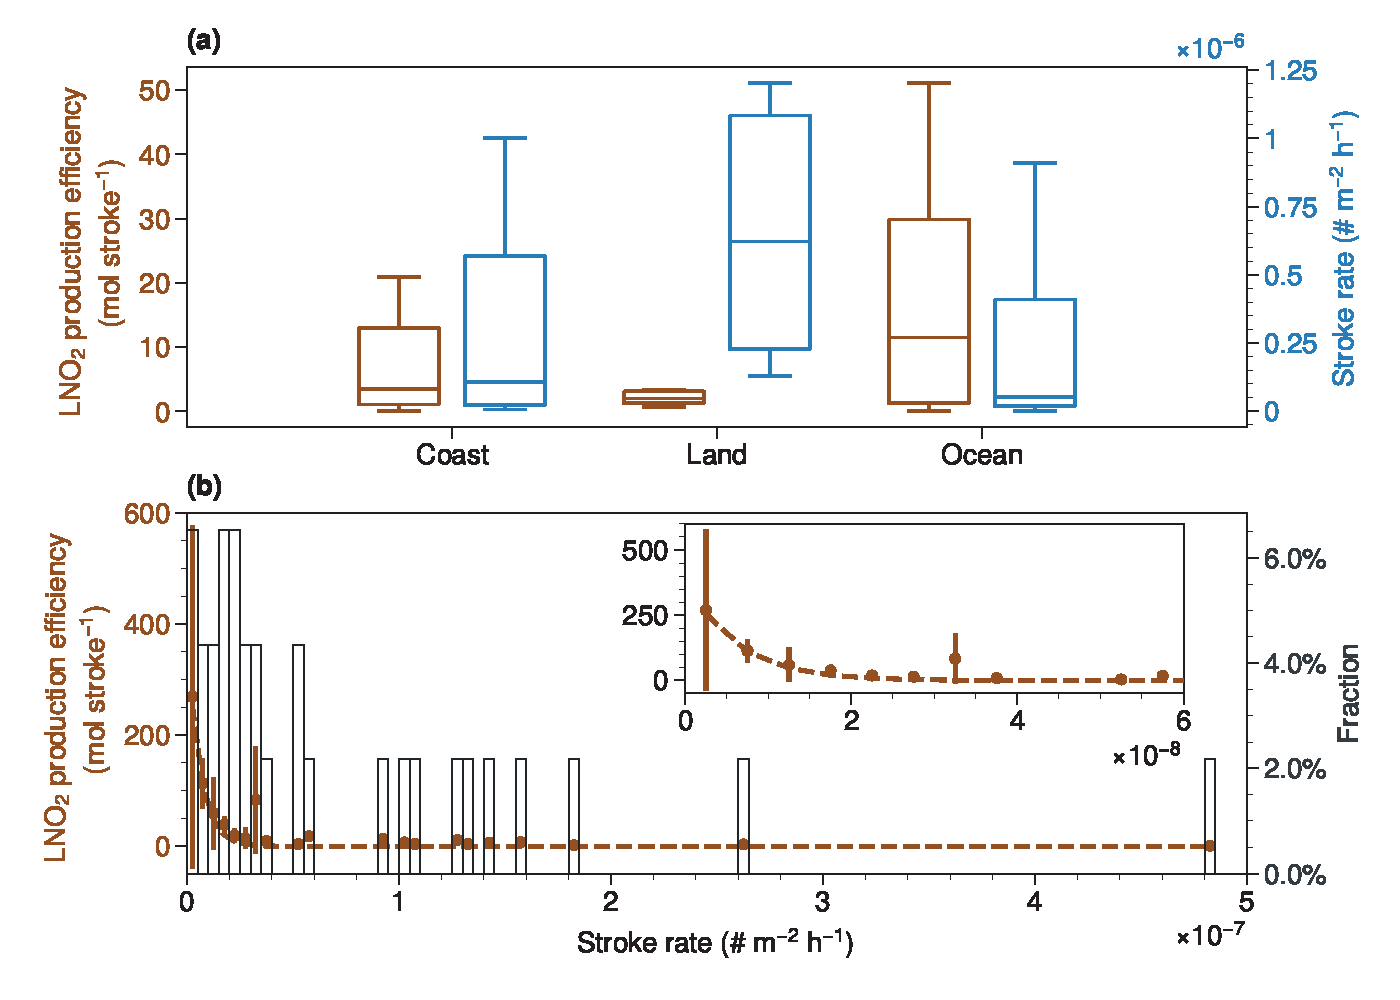
\includegraphics[width=0.9\textwidth]{./figures/arctic_pe_rate.png}
\caption{
(a)三个区域(沿岸、陆地和海洋)的LNO$_{\ch{2}}$产率(棕色)和闪击频率(蓝色),
其中沿岸地区为海岸线周围 500 m 的半径,详见图\ref{fig:arctic_region_mask}。
箱线图表示中值,下边界和上边界分别代表第 25 个和第 75 个百分位数,上下误差线分别代表第 10 个和第 90 个百分位数;
(b)LNO$_{\ch{2}}$ 产率与闪击频率的关系,叠加每个 5$\times$10$^{-9}$ m$^{-2}$ h$^{-1}$ 中个例占比的直方图。 \\
Figure \ref{fig:arctic_pe_rate}. (a) Comparison of lightning NO$_{\ch{2}}$ (LNO$_{\ch{2}}$) production efficiency (brown) and stroke rate (blue) for three regions: coast, land, and ocean.
The coast region is defined as a 500 m radius around the coastline (Details see Fig. \ref{fig:arctic_region_mask}).
The box plots indicate the median values; the lower and upper boundaries represent the 25th and 75th percentiles, respectively, and the lower and upper error lines are the 10th and 90th percentiles, respectively.
(b) LNO$_{\ch{2}}$ production efficiency vs stroke rate, with histograms of case fractions in each 5$\times$10$^{-9}$ m$^{-2}$ h$^{-1}$ stroke rate bin overlaid.
}
\label{fig:arctic_pe_rate}
\end{figure}

\subsection{氮氧化物不同排放源的贡献}


图 \ref{fig:arctic_no2_comp}a 为2019至2021 年 6--8 月 TROPOMI 在北极观测到的平均 NO$_{\ch{2}}$ 柱浓度分布图,
虽然从背景中无法看出LNO$_{\ch{2}}$,但在城市、工业和野火地区仍然可以观察到 NO$_{\ch{2}}$ 的增强。
例如与阿拉斯加、挪威和俄罗斯的采矿作业相关的 NO$_{\ch{2}}$ 柱浓度高值(17 $\pm$ 2 $\mu$mol m$^{-2}$),
石油和天然气活动也显现出明显的NO$_{\ch{2}}$高值,
如加拿大北极麦肯齐谷、北阿拉斯加普拉德霍湾/库帕鲁克和俄罗斯亚马尔天然气管道/乌连戈气田\citep{VanDerA.2020}。
而格陵兰海岸沿线的 NO$_{\ch{2}}$ 高值可能是与复杂地形反演相关的错误信号\citep{Hachmeister.2022}。
与 NO$_{\ch{2}}$ 污染相反,70$^{\circ}$ N 以北的 TROPOMI 观测显示背景 NO$_{\ch{2}}$浓度较低(4.35 $\pm$ 1.26 $\mu$mol m$^{-2}$),
比 60$^{\circ}$ N 和 65$^{\circ}$ N 之间的平均 NO$_{\ch{2}}$ 低45\%。

通过将每个个例中LNO$_{\ch{2}}$柱浓度的最大值(61 $\pm$ 50 $\mu$mol m$^{-2}$)与北极地区典型的人为和野火 NO$_{\ch{2}}$ 进行比较,
本研究发现 LNO$_{\ch{2}}$ 的柱浓度为其他源的3倍,尽管排放的时间尺度是小时数量级(图 \ref{fig:arctic_no2_comp}b)。
其中发生在拉普捷夫海(Laptev Sea)上空的深对流(图\ref{fig:arctic_large_lno2}),
其LNO$_{\ch{2}}$最大值 为 246 $\mu$mol m$^{-2}$,
与美国夏季最高 NO$_{\ch{2}}$ 柱浓度相当[234 $\mu$mol m$^{-2}$,\citet{Goldberg.2021a}]。
考虑到LNO$_{\ch{2}}$在短时间内的巨大贡献,因此计算北极地区LNO$_{\ch{2}}$排放显得十分重要。

\begin{figure}[H]
\centering
\includegraphics[width=0.9\textwidth]{./figures/arctic_no2_comp.png}
\caption{
(a)2019至2021年6--8月当地下午时TROPOMI测得的对流层 NO$_{\ch{2}}$ 平均柱浓度(4 km $\times$ 4 km);
(b)四种NO$_{\ch{2}}$来源的柱浓度比较:闪电、采矿、石油天然气和野火。
其中闪电NO$_{\ch{2}}$浓度为每次对流个例所有像素上NO$_{\ch{2}}$的最大值,
而野火、采矿和石油天然气的浓度是(a)中典型位置的每日NO$_{\ch{2}}$最大值。
框内的黑线和红线分别是中值和均值,
下边界和上边界分别是第 25 和第 75 个百分位数,
上下误差线分别是第 10 和第 90 个百分位数。\\
Figure \ref{fig:arctic_no2_comp}. (a) Mean 4 km $\times$ 4 km TROPOMI tropospheric NO$_{\ch{2}}$ column density in the local afternoon during June--August 2019--2021.
The mining and oil and gas stations are shown as gray and red circles, respectively.
(b) Comparisons of NO$_{\ch{2}}$ among four sources: lightning, mining, oil and gas, and wildfire.
The lightning bar represents the maximum NO$_{\ch{2}}$ values over pixels for each lightning case,
while the wildfire, mining, and oil and gas bars are the daily maximum NO$_{\ch{2}}$ values at typical locations.
The box plots indicate the median (black line) and mean (red line) values; the lower and upper boundaries represent the 25th and 75th percentiles, respectively, and the lower and upper error lines are the 10th and 90th percentiles, respectively.
}
\label{fig:arctic_no2_comp}
\end{figure}

\begin{landscape}
\vspace*{\fill}
\begin{figure}[H]
\centering
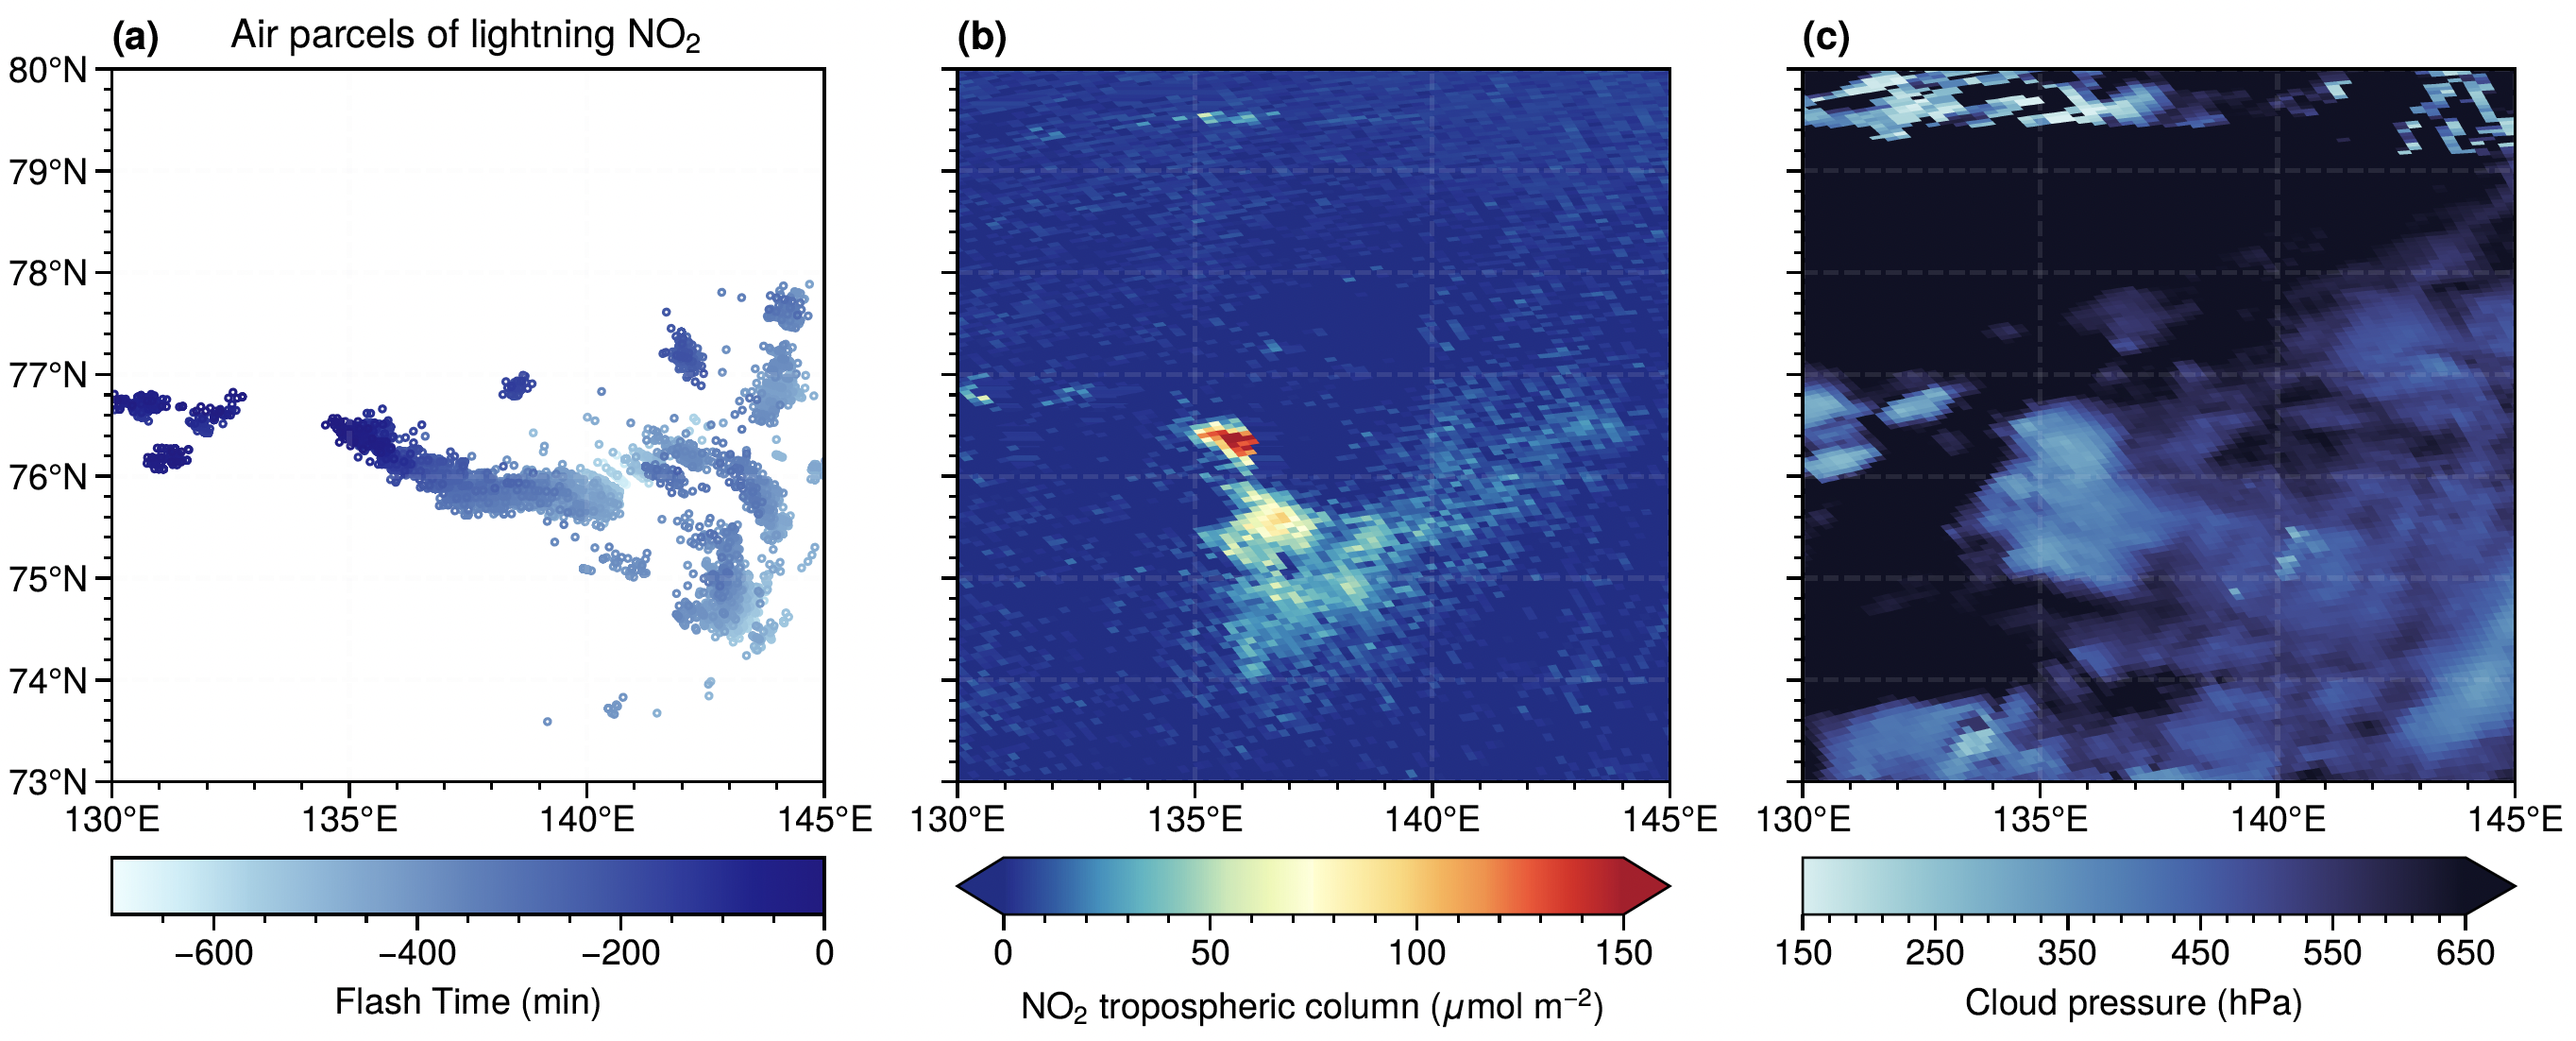
\includegraphics[width=0.9\columnwidth]{./figures/arctic_large_lno2.png}
\caption{
(a)在 500 hPa气压层水平传输的包含闪电 NO$_{\ch{2}}$ 的空气块;
(b)TROPOMI 观测到的 NO$_{\ch{2}}$ 对流层柱浓度;
(c)TROPOMI 观测到的云压。\\
Figure \ref{fig:arctic_large_lno2}. (a) Transported air parcels containing lightning NO$_{\ch{2}}$ at 500 hPa pressure level.
(b) The TROPOMI-detected NO$_{\ch{2}}$ tropospheric vertical columns.
(c) The TROPOMI-detected cloud pressures.
}
\label{fig:arctic_large_lno2}
\end{figure}
\vspace*{\fill}
\end{landscape}

\begin{landscape}
\vspace*{\fill}
\begin{figure}[H]
\centering

\includegraphics[width=0.9\columnwidth]{./figures/arctic_emission_comp.png}
\caption{
北极地区6--8月的NO$_{\ch{x}}$月排放量
(a)人为排放(包括船舶排放);(b)土壤排放;
(c)船舶排放。
闪电 NO$_{\ch{x}}$ 排放是 2019 年至 2021 年的平均值,
其他排放来自哥白尼大气监测服务(CAMS)2018 年全球排放清单。\\
Figure \ref{fig:arctic_emission_comp}. Monthly NO$_{\ch{x}}$ emissions in the Arctic from June to August.
(a) Anthropogenic emissions including ship emissions, (b) soil emissions, and (c) lightning emissions.
The lightning NO$_{\ch{x}}$ emissions are the mean values from 2019 to 2021, while the other emissions are from the 2018 Copernicus Atmosphere Monitoring Service (CAMS) global emission inventories.
}
\label{fig:arctic_emission_comp}
\end{figure}
\vspace*{\fill}
\end{landscape}

由于闪击频率计算所用到的面积取决于TROPOMI中LNO$_{\ch{2}}$的选区,
本研究将闪击数乘以三个地区各自的 LNO$_{\ch{2}}$ 产率的中值,并将它们相加作为北极地区($>$ 70$^{\circ}$ N)LNO$_{\ch{2}}$的总排放量(表\ref{table:arctic_emission})。
结果表明,2020 年 LNO$_{\ch{2}}$ 排放量为 109 吨氮,比 2019 年和 2021 年的 LNO$_{\ch{2}}$ 平均排放量(83 吨氮)高出 31\%,
70$^{\circ}$ N 和 80$^{\circ}$ N 之间增大35\%的排放是其主要贡献,
该区域的2020年平均对流有效位能(CAPE)比2019和2021年的均值高出 32\%
(表\ref{table:arctic_emission} ,图 \ref{fig:arctic_cape_aod})。
而北极点附近(80$^{\circ}$--90$^{\circ}$ N)由于闪电增多,LNO$_{\ch{2}}$ 排放量(4.3 吨氮)在 2021 年增加了 353\% (表 \ref{table:arctic_emission})。

假设 NO$_{\ch{x}}$ 与 NO$_{\ch{2}}$ 的比例为 2.4 \citep{Silvern.2018},计算得到 LNO$_{\ch{x}}$ 月排放量为 73 吨氮,
并将其与夏季北极地区的人为和土壤 NO$_{\ch{x}}$ 排放量进行比较(图\ref{fig:arctic_emission_comp})。
本研究发现土壤月排放总量为 2670 吨氮,是北极陆地上NO$_{\ch{x}}$的主要排放源,
而陆地上人为 NO$_{\ch{x}}$ 月排放量为350 吨氮与野火月排放量(430 吨氮)在同一量级。
此外船舶月排放总量为 1160 吨氮,是北极海洋上 NO$_{\ch{x}}$ 的主要来源,
然而LNO$_{\ch{x}}$在北极东北部海洋地区(90--180$^{\circ}$ E, 80--90$^{\circ}$ N)占比高达93\%。
由于对流层上层温度较低,远离雷暴处的NO$_{\ch{2}}$寿命为 $\sim$ 0.5--8 天\citep{Schumann.2007,Nault.2017},
故需要更多的研究来评估 LNO$_{\ch{2}}$对O$_{\ch{3}}$、CO 和 CH$_{\ch{4}}$的影响。


本节研究的局限性为LNO$_{\ch{2}}$ 产品是在没有反演LNO$_{\ch{2}}$垂直廓线的情况下得出的LNO$_{\ch{2}}$柱浓度。
虽然云切片技术\citep{BelmonteRivas.2015,Marais.2021}可以从 TROPOMI 观测中推导出 LNO$_{\ch{2}}$ 廓线,
但它们需要大样本量来降低噪点。
未来的飞机观测,如深对流云和化学项目[DC3,\citet{Barth.2019}],
可以提供更详细的 LNO$_{\ch{2}}$ 廓线,并提高本研究对北极地区空气污染和气候变化的理解\citep{Law.2007,Schmale.2018}。

由于预计北极闪电会随着全球变暖而增加,因此准确的闪电观测、模拟和验证对于 LNO$_{\ch{2}}$ 的分析非常重要。
由于北极大部分地区被海洋或冰覆盖,地基闪电探测网的探测效率仍然很低\citep{Vagasky.2022}。
此外北极目前可用的闪电参数化主要集中在陆地,尤其是永冻区\citep{Chen.2021a},
因此一致的卫星观测(例如 OTD)对于北极闪电研究至关重要。
虽然热带降雨测量任务[TRMM,\citet{Cecil.2014}]和国际空间站[ISS,\citet{Blakeslee.2020}]上都配备了闪电成像传感器(LIS),
但是它们只探测热带和中纬度闪电,
其中TRMM LIS 覆盖低纬度($\pm$ 38$^{\circ}$),ISS LIS 的覆盖范围扩展到更高纬度($\pm$ 55$^{\circ}$)。
未来计划中的闪电传感器可以探测的纬度范围目前尚不清楚,
然而若将水文气象卫星[例如 Arktika-M,\citet{Asmus.2021}]
与闪电传感器[例如全球闪电测绘仪(GLM)和闪电测绘成像仪(LMI),\citet{Goodman.2013,Yang.2017}] 相结合,可以帮助我们更好地了解北极闪电的变化。


\begin{figure}[H]
\centering
\includegraphics[width=\textwidth]{./figures/arctic_cape_aod.png}
\caption{
2019至2021年6--8月平均 GLD360 闪击频率、对流有效位能(CAPE,来自 ERA5)和气溶胶光学厚度(550 nm 处的 AOD,来自 MERRA-2)。\\
Figure \ref{fig:arctic_cape_aod}.
Mean GLD360 lightning stroke rate, convective available potential energy (CAPE, from ERA5), and aerosol optical depth (AOD at 550 nm, from MERRA-2) during June--August 2019–-2021.
}
\label{fig:arctic_cape_aod}
\end{figure}


% \begin{figure}[H]
% \centering
% 
\includegraphics[width=\textwidth]{./figures/arctic_emission_comp.png}
% \caption{
% 北极地区6--8月的NO$_{\ch{x}}$月排放量
% (a)人为排放(包括船舶排放);(b)土壤排放;
% (c)船舶排放。
% 闪电 NO$_{\ch{x}}$ 排放是 2019 年至 2021 年的平均值,
% 其他排放来自哥白尼大气监测服务(CAMS)2018 年全球排放清单。\\
% Figure \ref{fig:arctic_emission_comp}. Monthly NO$_{\ch{x}}$ emissions in the Arctic from June to August.
% (a) Anthropogenic emissions including ship emissions, (b) soil emissions, and (c) lightning emissions.
% The lightning NO$_{\ch{x}}$ emissions are the mean values from 2019 to 2021, while the other emissions are from the 2018 Copernicus Atmosphere Monitoring Service (CAMS) global emission inventories.
% }
% \label{fig:arctic_emission_comp}
% \end{figure}

\section{本章小结}

本章建立了基于卫星遥感NO$_{\ch{2}}$柱浓度定量分析污染和清洁背景下LNO$_{\ch{2}}$的计算方法,
得到了污染和清洁地区的LNO$_{\ch{2}}$产率,并与其他NO$_{\ch{x}}$排放源进行了对比。主要结论如下:

\begin{enumerate}[label=(\arabic*), labelindent=\parindent, nosep, leftmargin=0pt, widest=0, itemindent=*, topsep=0pt, partopsep=0pt, parsep=0pt]

\item 2019年和2020年中国东部的两个对流个例分析表明,TROPOMI 的像素饱和效应
限制了对流旺盛区域的LNO$_{\ch{2}}$浓度估计,
因此本研究提出了计算消散阶段LNO$_{\ch{2}}$的方法。
通过该方法,我们得出了中国东部的LNO$_{\ch{x}}$产率为 60 $\pm$ 33 mol NO$_{\ch{x}}$每闪电。
未来的研究可同时利用对流旺盛和消散期间 OMI或TROPOMI 的有效数据,进一步量化和改进 LNO$_{\ch{x}}$ 的产量估计。

\item 本章还进行了敏感性试验,通过在WRF-Chem模式中设置不同的LNO$_{\ch{2}}$产率来代入TROPOMI NO$_{\ch{2}}$柱浓度的计算,
发现LNO$_{\ch{2}}$的贡献在新生闪电区会导致AMF$_{\ch{trop}}$下降23\%,而在出流区和老化区会增加60\%。

\item 针对清洁地区(北极)的深对流,本章利用极轨卫星在北极地区连续过境的特性,
开发了TROPOMI LNO$_{\ch{2}}$柱浓度高值区的自主识别系统,提出了通过相邻过境数据来定量计算 LNO$_{\ch{2}}$ 寿命和产率的方法。
分析结果显示,2019至2021年夏季北极地区对流附近的LNO$_{\ch{2}}$寿命为3 h,
与污染地区的LNO$_{\ch{2}}$寿命相似,例如美国地区的3 h \citep{Nault.2017}。
北极陆地地区的LNO$_{\ch{2}}$ 产率 [2.0(1.3--3.1)mol每闪击] 与\citet{Lapierre.2020}在美国的研究结果(1.6 $\pm$ 0.1 mol每闪击)相近,但相当于本研究在美国大陆得出的结果(6 $\pm$ 3 mol每闪击)的最小值。
此外,北极海洋性闪电产生的 NO$_{\ch{2}}$是陆地性闪电的6倍,
因此,当闪电在北极海洋和陆地上增加相同数量时,海洋性闪电将产生更多的 LNO$_{\ch{2}}$。
基于以上产率,本章进一步得出北极地区夏季LNO$_{\ch{x}}$ 的平均排放量为219吨氮,
约等于该地区人为 NO$_{\ch{x}}$ 排放量的 5\%。

\end{enumerate}


